%\documentclass[a4paper,10pt]{article}
\documentclass[acmcsur,acmnow]{acmtrans2m}
%\documentclass[acmtocl,acmnow]{acmtrans2m}

%\acmVolume{V}
%\acmNumber{N}
%\acmYear{YY}
%\acmMonth{Month}

% packages
\usepackage[utf-8]{inputenc}
\usepackage{paralist}
\usepackage{subfigure}
\usepackage{graphicx}
\usepackage{colortbl}
\usepackage{color,soul}
\usepackage{longtable}
\usepackage{wasysym}
\usepackage{pdflscape}
%\usepackage{tikz}
\usepackage{pgfplots}

% definitions
\newtheorem{theorem}{Theorem}[section]
\newtheorem{conjecture}[theorem]{Conjecture}
\newtheorem{corollary}[theorem]{Corollary}
\newtheorem{proposition}[theorem]{Proposition}
\newtheorem{lemma}[theorem]{Lemma}
\newdef{definition}[theorem]{Definition}
\newdef{remark}[theorem]{Remark}

%\newtheorem{theorem}{Theorem}[section]
%\newtheorem{definition}[theorem]{Definition}

%\textwidth      6.5in
%\textheight     9.2in
%\oddsidemargin  -0.5cm
%\evensidemargin -0.5cm
%\parindent      0pt              
%\topmargin      -0.3in
%\headsep        20pt
%
%\parskip        5pt
%\parindent      10pt

\markboth{}{}{}

\title{Alleviating the Topology Mismatch Problem in Unstructured and Structured
Overlay Networks: A Survey}
% TODO: We added here "P2P". I'm not sure, because for example Narada is not P2P
% TODO: I deleted "P2P"

\author{
VASSILIS S. MOUSTAKAS$^1$, H\"USEYIN AKCAN$^2$, MEMA ROUSSOPOULOS$^1$ and ALEX
DELIS$^1$\\
$^1$\emph{National and Kapodistrian University of Athens}, \emph{Athens},
\emph{Greece}\\
$^2$\emph{Izmir University of Economics}, \emph{Izmir}, \emph{Turkey}
}

\begin{abstract}
Peer-to-peer (P2P) systems is a rapidly growing application architecture. The
overlay network abstraction on top of a best-effort infrastructure provides a
powerful tool to realize a plethora of ever-wanted exotic features like
anonymity, high availability and robustness, load balancing, quality-of-service
(QoS) at the application layer and many more. Unfortunately weaknesses of early
effectuations constrained applications from unleashing the full potential of the
paradigm. One of them is the topology mismatch problem between the overlay and
the physical underlying network, a problem that imposes a huge amount of
unnecessary stress to the network resources and, thus, impede applications from
scaling. In this survey we investigate on the recent research developments
towards the alleviation of this problem, in both unstructured and structured
overlay architectures. We visit the various algorithms available in the
lietrature, focusing on the presentation of how each of them tries to tackle the
problem. Additionally, we provide a finer grained categorisation of the
approaches based on the generic type of methodology they use in order to
accomplish this goal.
% TODO: Review this after the comparison sections are fixed.
Finally we discuss the advantages, disadvantages and novelties introduced by the
algotithms and offer pictorial comparisons for them in order to further
strengthen and organise understanding of the information and knowledge cited, in
an attempt to make this survey a one-stop-shop reference for anyone interested
in the topic, from researchers and students, to system architects and
developers.
\end{abstract}

\category{A.1}{General Literature}{Introductory and Survey}
\category{C.2.4}{Distributed Systems}{Distributed Applications}

\terms{Topology mismatch}

\keywords{Distributed systems, peer-to-peer architectures, overlay network,
topology awareness}

\begin{document}

\begin{bottomstuff}
Authors' addresses: Department of Informatics and Telecommunications, National
and Kapodistrian University of Athens, Athens, Greece. Department of Software
Engineering, Izmir University of Economics, Izmir, Turkey.\\
emails: \{b.moystakas,mema,ad\}@di.uoa.gr, huseyin.akcan@ieu.edu.tr
\end{bottomstuff}

\maketitle

\section{Introduction}
\label{section:intro}

\IEEEPARstart{P}{eer-to-peer (\p)} networks are self-organizing, distributed systems where
participating nodes, called \emph{peers}, act as both resource providers and
resource consumers in contrast to the conventional \emph{client-server} model
where nodes undertake specific roles.
For over a decade, \p\ networks have been widely deployed and have
enjoyed immense popularity from Internet communities, primarily because
of the great number of features they offer to distributed applications 
built atop them. 
Such diverse features include:  high availability and robustness,
load-balancing, quality of service, scalability, decentralized administration,
and anonymity. 

The peer-to-peer paradigm gave impetus to two ``killer'' applications:
file-sharing and Internet telephony.
The {\sl Napster} file-sharing system was widely acknowledged as the 
``fastest growing Internet application ever'' in $2001$ when it topped
$26$ million users sharing over $80$ million songs.
Other file-sharing applications followed suit, 
including {\sl Gnutella} and {\sl Limewire} enjoying $3$ 
million concurrently-connected peers, as well as 
{\sl BitTorrent} connecting over $150$ million monthly users by January $2012$~\cite{bittorrentusers}.
\p\ telephony saw explosive growth with the advent of {\sl Skype}.
Since its introduction in $2003$,
{\sl Skype} has become extremely popular with more than $650$ million users 
in $2011$~\cite{skypetotalusers} and an astonishing 
$50$+ million concurrently-online users~\cite{skypesymusers}.
Moreover, it has consistently eroded  the traffic handled by 
traditional telephony carriers by slicing away a staggering 
$214$ billion minutes of pertinent traffic in $2013$ alone~\cite{skypetraffic}.

%%
Apart from the above, a startling number of diverse and successful
applications have been built based on \p\ architectures. Some of them include:
distributed search engines~\cite{yaci}, 
distributed data-storage systems~\cite{kbc_oceanstore_2000,bdet_fsdfs_2000,dkkms_cfs_2001,dr_pastutility_2001,abc_farsite_2002,mmfc_ivy_2002,arla,agebh_dks_2003},
Web caches, archives and publishing systems~\cite{ird_squirrel_2002,bags_youserv_2002,wrc_publius_2000,wm_tangler_2001},
messaging and dissemination applications~\cite{threedegrees,icpp08-pd}, 
event-notification infrastructures~\cite{rkcd_scribe_2001,cdkr_scribe_2002,agebh_dks_2003}, 
naming services~\cite{cmm_chorddns_2002}, 
censor-resistant stores~\cite{cswh_freenet_2001} and
lately, even cloud-based platforms~\cite{mgpj_cloudsnap_2011}.

\p\ systems are implemented using \emph{overlay networks}. 
An overlay network, is a virtual system of nodes featuring logical interconnects (or links)
created above an existing network; overlays provide an abstraction that
enables the implementation of efficient, fully distributed, application-layer
services such as routing messages to destinations that are not known in advance
or offering QoS guarantees (i.e., in content-distribution) over best-effort
infrastructures. Overlay nodes communicate through \emph{virtual connections}
each of which may correspond to a path of possibly many physical links 
in the underlying network.
Figure~\ref{figure:overlay} illustrates a simple four-node overlay constructed
over a wide-area network.
%%
\begin{figure}[ht]
\centering
  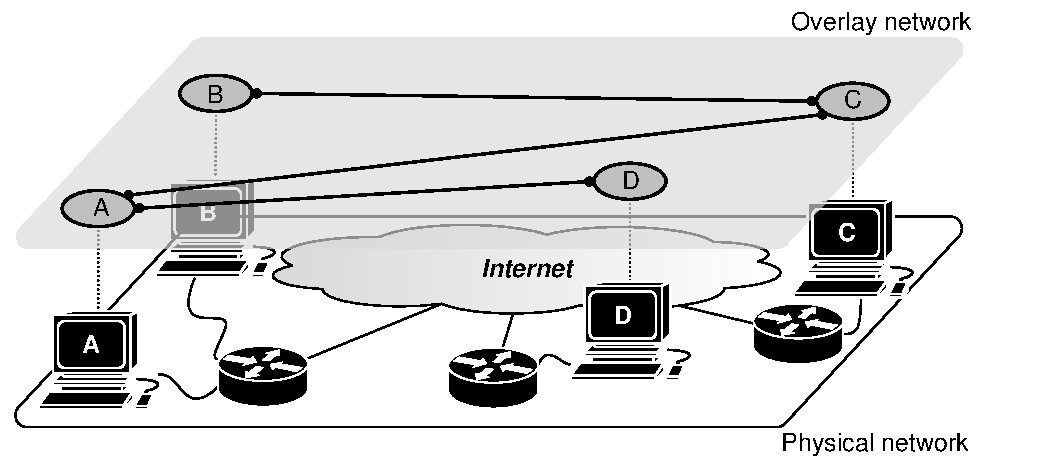
\includegraphics[scale=0.45]{img/pdf/under-over-lay.pdf}
\caption{An example overlay network.}
\label{figure:overlay}
\end{figure}

The single key issue that determines the efficiency of an overlay network,
is how well the overlay maps to the underlying network topology on which it
``rests''. 
Consider two nodes\footnote{In \p\ networks,
the participating nodes are typically user-PCs operating at the edge of the
Internet.} that are connected with each other via a path of overlay links.
If the application running on the nodes, generates heavy traffic along
the overlay path, it would be beneficial to
construct the overlay topology in a way that the number of 
underlying IP links between these two nodes is minimized.
Should the overlay network be constructed so that
it does not match the underlying topology well, 
the inherent \emph{topology mismatch} creates two
major problems. 
First, the performance of the application per se, can be
adversely affected since traffic must flow over a larger,
redundant, number of physical hops resulting in poor user experience 
entailing noticeable latencies or jitter. 
%%
Second, other applications running
on the underlying network infrastructure may be adversely affected as well.
Studies have shown that highly popular \p\ applications contribute 
the largest portion of the overall 
Internet traffic~\cite{seroiu_analysiscds_2002,sen_analyzep2ptraffic_2004,krp_ispfear_2005}, with some reporting that more than $60$\% of this traffic 
to be \p-related~\cite{cachelogic,ipoque2009};
it was also projected that this traffic would reach
$7$~\emph{Exabytes}-per-month by $2018$~\cite{CVNI2014}! 
This constitutes a major burden for 
Internet Service Providers (ISPs) who must route 
all of this traffic to destinations at the edge of the Internet. 
If the \p\ overlay topology is poorly designed, 
the demand on the Internet's backbone infrastructure may 
substantially increase as traffic might have to flow
``back and forth'' several times between two neighboring ISPs
while trying to travel from the source to its destination node
in the overlay.
Hence, it is critical that \p\ networks be laid out 
in ways that their topology matches the underlying IP topology as 
closely as possible.

For over a decade, researchers have extensively investigated  
various aspects of the topology mismatch problem.
This research area started to become active after  The mismatch problem is Interest around All interesting work around the topology We omitted centralized Centralized systems are not 

The main objective of this paper is to offer a comprehensive 
survey of the work carried out in the area
and provide a
taxonomy of the proposed solutions. We point out synergies, as well as
similarities and differences in the published approaches. 
Ultimately, our goal is to help readers sift through 
the voluminous literature, to help them
understand the advantages and disadvantages of each work, and 
to provide them with enough perspective so that 
when the need arises, they are able to
select, amongst the different approaches, the one that is most suitable for
their particular application.
%%
The rest of the paper is organized as follows: 
In Section~\ref{section:background}, we provide background on
overlay architectures including centralized, decentralized-unstructured and
decentralized-structured \p\ systems.
We also formally define the problem of topology mismatch 
and offer the rationale behind our 
evaluation of the techniques discussed in this paper. 
Work in the area was inspired mostly by the volatile and fully
distributed nature of the decentrilized overlays so we skip
centralized systems and in Sections~\ref{section:unstructured} and~\ref{section:structured}
we outline the surveyed research efforts
for unstructured and structured \p\ overlays, respectively.
We conclude in Section~\ref{section:conclusion}.

\section{Background}
\label{section:background}

%The abstraction of the overlay network has been proposed as a way to implement
%efficient, fully distributed, application-layer services such as  
%routing messages to destinations that are not known in advance or building
%one-to-many addressing schemes 
% TODO find citation for Narada & Adobe's Real Time Media Flow Protocol (RTMFP)
%\cite{} that provide quality-of-service (QoS) guarantees. \emph{IP
%multicast}, as well as other proposals such as \emph{IntServ} and
%\emph{DiffServ} \cite{cisco_diffserv_2005}, have still not seen wide deployment
%largely due to the fact they require support from the IP
%infrastructure. On the other hand, an overlay network can be deployed on
%end-systems running the overlay protocol software, without the cooperation of ISPs.
%Academic research includes
%\cite{chu_esm_2000,jannotti_overcast_2000,kwon_tag_2002} among others.

In this section, we provide some background information on the types of
peer-to-peer architectures that have been implemented and deployed. We also
describe and motivate more formally the topology mismatch problem tackled by
many P2P researchers over the past several years.

%%%%%%%%%%%%%%%%%%%%%%%%%%%%%%%%%%%%%%%%%%%%%%%%%%%%%%%%%%%%%%%%%%%%%%%%%%%%%%%%
%%%%%%%%%%%%%%%%%%%%%%%%%%%%%%%%%%%%%%%%%%%%%%%%%%%%%%%%%%%%%%%%%%%%%%%%%%%%%%%%
\subsection{Peer-to-Peer (P2P) Overlay Architectures}
%%%%%%%%%%%%%%%%%%%%%%%%%%%%%%%%%%%%%%%%%%%%%%%%%%%%%%%%%%%%%%%%%%%%%%%%%%%%%%%%
%%%%%%%%%%%%%%%%%%%%%%%%%%%%%%%%%%%%%%%%%%%%%%%%%%%%%%%%%%%%%%%%%%%%%%%%%%%%%%%%
Circa 2000, the first P2P file-sharing systems introduced the \emph{servent}
concept \cite{gnutella}, a \emph{portmanteau} that blends the notions of server
and client to denote the twofold role of a node participating in the P2P
network. Such server-less systems have proven to be able to achieve outstanding
aggregate resource capacities as more and more participants join the system
without requiring additional expenditure for infrastructure. While certain
undesirable features such as 
free-riding~\cite{saroiu_measurefileshare_2002,adar_gnutellafreeriders_2000,hughes_gnutellafreeride_2005},
the distribution of illegal content and other \emph{socio-technical}
issues \cite{hughes_socp2p_2008}, have arisen, peer-to-peer systems have
continued to gain popularity mainly because they have successfully supported
popular applications (i.e. file-sharing) amongst vast numbers of participating
users.

For over a decade, excitement over the immense potential of P2P systems has
generated a flurry of research and development, resulting in a wide range of
popular protocols, networks, and applications. As P2P systems evolved, three
main architectures have emerged, namely
\begin{inparaenum}[\itshape i\upshape)]
  \item \emph{centralized},
  \item \emph{decentralized unstructured}, and
  \item \emph{decentralized structured}.
\end{inparaenum}

Designers of \emph{centralized} architectures (see
Figure~\ref{figure:p2p-archs:centralized}) were the first to recognize that
requests for resources (e.g. CPU cycles or popular content) need not be sent to
a dedicated server but instead could be handled by the many hosts that already
posses the resources. The downside of this approach is that it requires a
centralized searching facility which becomes a single point of failure, a
scalability bottleneck, and a target of malicious attacks (e.g.,
\emph{Denial-of-Service (DoS) attacks}).

The most successful incarnation of the centralized approach is the file-sharing
application \emph{Napster}\cite{napster}. Napster maintained a \emph{central
index server} based on file lists provided by participating peers. The central
index server was queried by users and it returned pointers to the actual
content. Thus, by centralizing search while distributing downloads,  Napster
achieved a highly functional design that, at its height, attrated 26 million
users sharing approximately 80 million songs\cite{jmm_naptopusage_2001}.
Napter's  centralized nature was what ultimately brought it down after Recording
Industry Association of America (RIAA) filed a lawsuit for copyright infringemnt
of the intellectual property of artists whose music was distributed by the
Napster application. RIAA was able to point to the centralized indexing
component of Napster as the entity resposible for illegal song-trading.
                                       
The centralized approach was quickly replaced by architectures that distribute
both search and resource provision capabilities (see
Figure~\ref{figure:p2p-archs:unstructured-full}). In these \emph{decentralized}
architectures, resource placement within the overlay topology is
random~\cite{YG-M2002}. For this reason they are referred to as
\emph{unstructured}. The most important properties of such systems are that they
support inherent heterogeneity of peers, are highly resilient to peer failures,
and incur low maintenance overhead at handling the dynamics of peer
participation \cite{stutzbach_churn_2006}. In the literature, they are also
known as \emph{broadcast-based} systems, because they use message flooding among
peers to propagate search queries. A well-known example of the fully
decentralized
unstructured approach is Gnutella, in its first realization (v.0.4)
\cite{gnutellav04}.

A key disadvantage of the unstructured approach is that message flooding burdens
the network since queries travel within the network randomly, visiting nodes
that do not have the resource of interest and thus wasting bandwidth.  To save
on bandwidth, unstructured networks typically limit how long a query travels
within the overlay (via a time-to-live (TTL) parameter). When a query is
received by a node, it decreases the TTL by one unit. If the TTL has not reached
zero, the node forwards the query to its neighbors.  Otherwise, it drops the
query. While this approach prevents queries from visiting the entire network, it
does not guarantee that the resource of interest, (e.g., a rare recording 
of a musical group from the 1930s) will be found.

To improve search scope and scalability and to lighten network load, 
unstructured systems evolved into ``hierarchical'' systems that dynamically
assign indexing functions to special peers, called \emph{ultra-peers}  or
\emph{super-peers} (see
Figure~\ref{figure:p2p-archs:unstructured-hierarchical}). Peers with reliable
network connections and/or high compute power became ultra/super-peers
facilitating less powerful peers (called \emph{leaf-nodes}) to find resources of
interest. Well-known examples of these hierarchical unstructured systems include
Gnutella v.0.6/Limewire~\cite{gnutella}, KaZaA~\cite{kazaa} and
Skype~\cite{skype}. While the hierarchical approach relieves network pressure as
search queries are flooded over a much smaller subset of peers (the
ultra/super-peers), the disadvantages of reduced search scope and inability to
locate rare resources efficiently remain.

To fully address the disadvantages of decentralized unstructured approaches,
\emph{decentralized structured} schemes have been proposed (see
Figure~\ref{figure:p2p-archs:structured}). The key goal of these systems is to
provide a self-organizing infrastructure for large-scale P2P applications
\cite{ratnasamy_can_2001,stoica_chord_2001,antony_pastry_2001,zhao_tapestry_2001,maymounkov_kademlia_2002,rgrk_bamboo_2004}.
They implement a \emph{Distributed Hash Table (DHT)} that maps objects to nodes
through a deterministic mechanism. The DHT provides a guaranteed bound on the
number of overlay routing hops that have to be taken to locate a resource, even
in the case when only a single copy exists in the system.  This means
$O \left( log n \right)$ hops, compared to unstructured networks that require
$O \left( n \right)$ to reliably locate any object. Unfortunately this
efficiency does not come without cost. Structured overlays can only support
exact-match queries (i.e., queries that identify resources by name) as opposed
to content-based retrieval provided by unstructured overlays. This means
that unstructured overlays can support more versatile resource location queries
such as keyword and partial matching searches. Several popular file-sharing
peer-to-peer applications have been based on DHTs including
Overnet/eDonkey~\cite{overnet}, Kademlia/Kad
Network~\cite{maymounkov_kademlia_2002}, some flavors of
BitTorrent~\cite{c_bittorrent_2003}, and many more.  Moreover, DHTs have sparked
a flurry of research activity and development for a large range of applications:
from distributed search engines to event notification infrastructures to
cloud-based platforms. We cite several examples in Section~\ref{section:intro}.

\begin{figure}[ht]
\centering
\subfigure[Centralized (SETI@Home or Napster). Peers query the centralized
entity (dotted lines) and then establish the connection to the data source.] {
  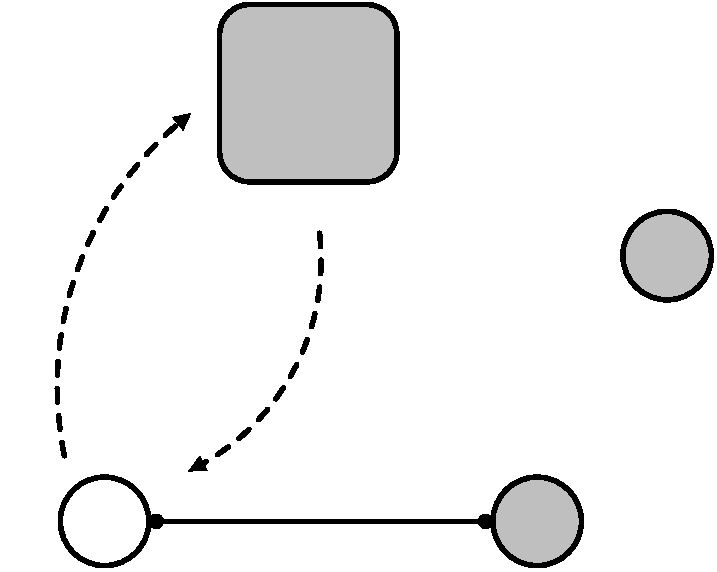
\includegraphics[scale=0.25]{img/pdf/centralized.pdf}
  \label{figure:p2p-archs:centralized}
}\qquad\qquad
\subfigure[Fully unstructured (Gnutella v.0.4). Data is distributed randomly,
the topology is also random and all participants are equal.] {
  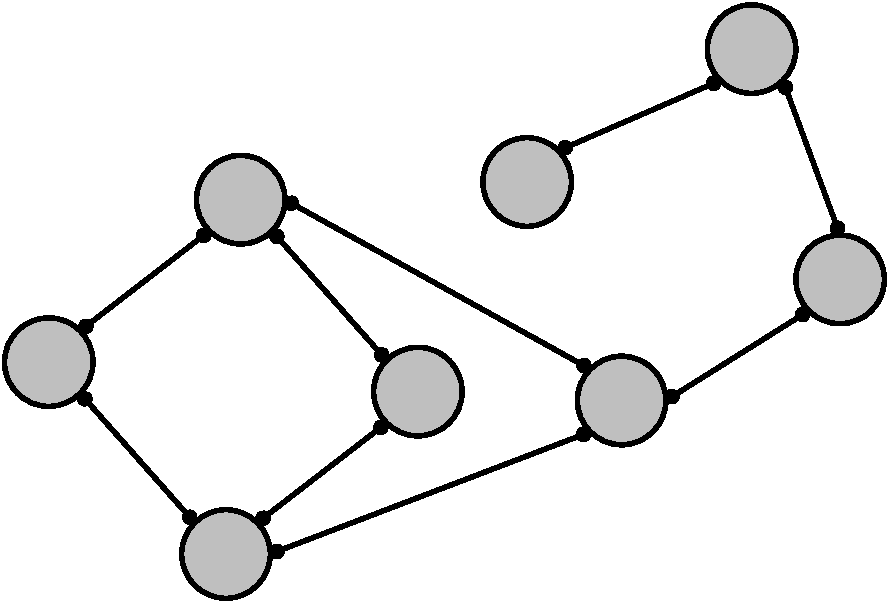
\includegraphics[scale=0.25]{img/pdf/unstructured-full.pdf}
  \label{figure:p2p-archs:unstructured-full}
}\qquad\qquad
\subfigure[Hierarchical unstructured (Gnutella v.0.6 or FastTrack). Certain
peers (bigger circles) shoulder specific responsibilities (e.g., data
indexing).] {
  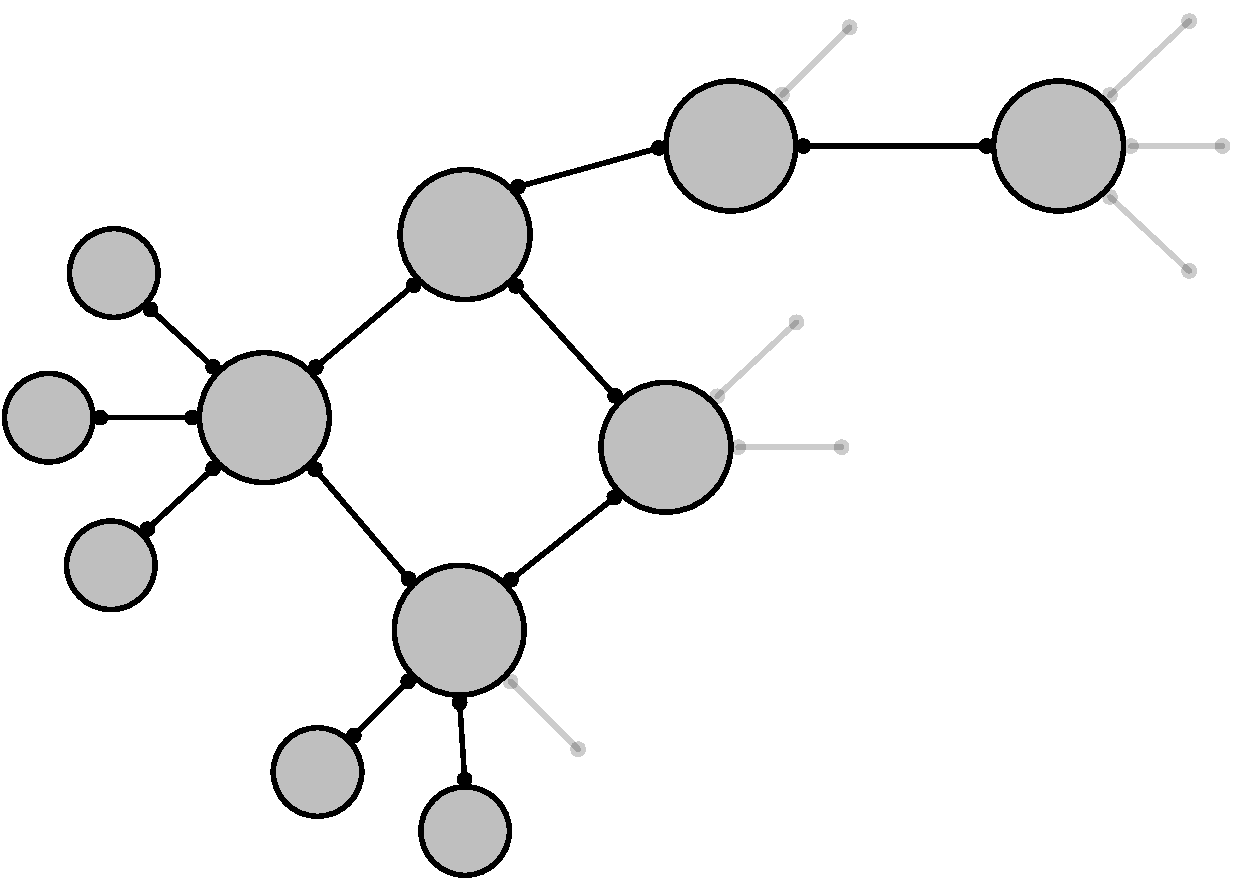
\includegraphics[scale=0.25]{img/pdf/unstructured-hierarchical.pdf}
  \label{figure:p2p-archs:unstructured-hierarchical}
}\qquad\qquad
\subfigure[Structured (Chord and Kademlia). Peers and data are placed into the
overlay in a deterministic manner.] {
  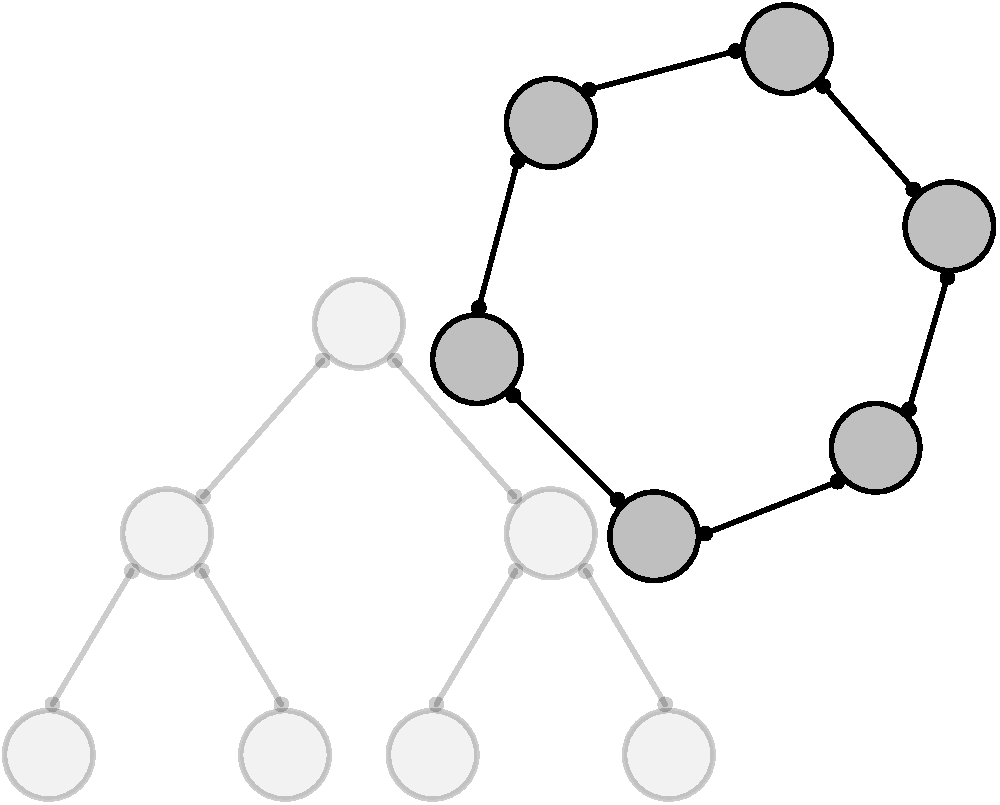
\includegraphics[scale=0.25]{img/pdf/structured.pdf}
  \label{figure:p2p-archs:structured}
}
\caption{The various peer-to-peer architectures.}
\label{figure:p2p-archs}
\end{figure}

%%%%%%%%%%%%%%%%%%%%%%%%%%%%%%%%%%%%%%%%%%%%%%%%%%%%%%%%%%%%%%%%%%%%%%%%%%%%%%%%
%
% TODO: SOME DISCUSSION ON P2P ARCHITECTURES
%
%\cite{matei_mapgnutella_2002, lv_randomwalks_2002, merugu_str2unstr_2003}
%showed that the ad-hoc network topology of unstructured overlay networks that
%preserve \emph{Power Law} and \emph{Small World} characteristics\footnote{Power
%Law describes the node degree while the Small World describes characteristics
%of path length and clustering coefficient. The clustering coefficient for a
%node $\upsilon$ in a graph $G = \left( V, E \right)$ is defined as the ratio of
%the existing connections between $\upsilon$'s neighboring nodes to $\gamma
%\times \left( \gamma - 1 \right)$, where $\gamma$ is the number of neighboring
%nodes of $\upsilon$. High cluster coefficient means that neighboring nodes of
%any node $\upsilon$ likely connect one another.} \cite{faloutsos_powerlaw_1999,
%saroiu_measurefileshare_2002} offer a more promising approach. Particularly:
%\begin{itemize}
%  \item Peer-to-peer clients are extremely \emph{transient}. Unstructured
%systems can have high maintenance traffic in delivering messages, updating the
%mapping, discovering failures and replicating lost data or pointers, making
%them insufficient on highly volatile networks.
%  \item \emph{Keyword searches} versus \emph{exact-match queries}. In DHTs
%there is a tight control between the data placement and the topology of the
%network. For this reason it is hard to efficiently support partially matched
%queries while Gnutella and other similar systems effortlessly support keyword
%searches and other complex queries since the mechanism is realized locally, on
%a node-by-node basis.
%  \item Popular content is located at multiple peers and thus it is more likely
%for a flooding-based search to return results. DHTs, on the other hand, fit
%better in the systems which require ability to reliably locate content, even in
%the extreme case that only a single-copy exists in the network.
%\end{itemize}

%
% TODO: SOME DISCUSSION ON THE ADVANTAGES OF UNSTRUCTURED NETWORKS FROM
%       \cite{z-yk_ddno_2005}
%
%Unstructured P2P networks o?er a number of
%important advantages: (i) An unstructured network
%imposes very small demands on individual nodes,
%and more speci?cally it allows nodes to join or leave
%the network without signi?cantly a?ecting the sys-
%tem performance. (ii) Unstructured networks are
%appropriate for content-based retrieval (e.g., key-
%word searches) as opposed to object identi?er loca-
%tion of structured overlays. (iii) Finally unstructured
%networks can easily accommodate nodes of vary-
%ing power. Consequently, they scale to very large
%sizes and they o?er more robust performance in
%the presence of node failures and connection
%unreliability.
%

%
% TODO: SOME DISCUSSION ON STRUCTURED OVERLAYS PROBABLY FROM
%       \cite{WLH2007}
% However, the design of a decentralized but structured P2P network has to
% overcome two critical issues. The first issue is the long routing latency.
% Several proximity schemes  have been proposed to avert long routing latency in
% current structured P2P networks, but they require a high-complexity procedure
% to periodically maintain the routing table (e.g. Pastry system) or they need
% pre-chosen landmarks to construct the overlay. However, the P2P system is by
% its very nature unstable since nodes join and leave frequently. For instance,
% the study of Gnutella shows around approximately 1200 membership changes per
% minute in a 100 000 nodes P2P system. Another proximity scheme needs some
% pre-chosen landmarks or a complete BGP routing table support. As a result,
% they both increase the difficulty of the P2P system deployment. The second
% issue is system maintenance overhead. The existing structured P2P networks
% allow nodes to keep some nearby nodes in their routing tables in order to
% achieve efficient routing.
%


%%%%%%%%%%%%%%%%%%%%%%%%%%%%%%%%%%%%%%%%%%%%%%%%%%%%%%%%%%%%%%%%%%%%%%%%%%%%%%%%



%%%%%%%%%%%%%%%%%%%%%%%%%%%%%%%%%%%%%%%%%%%%%%%%%%%%%%%%%%%%%%%%%%%%%%%%%%%%%%%%
%%%%%%%%%%%%%%%%%%%%%%%%%%%%%%%%%%%%%%%%%%%%%%%%%%%%%%%%%%%%%%%%%%%%%%%%%%%%%%%%
\subsection{The Topology Mismatch Problem}
%%%%%%%%%%%%%%%%%%%%%%%%%%%%%%%%%%%%%%%%%%%%%%%%%%%%%%%%%%%%%%%%%%%%%%%%%%%%%%%%
%%%%%%%%%%%%%%%%%%%%%%%%%%%%%%%%%%%%%%%%%%%%%%%%%%%%%%%%%%%%%%%%%%%%%%%%%%%%%%%%

One of the major issues that defines the efficiency of an overlay network is the
mapping of the overlay structure to the underlying infrastructure. Remember, in
Figure~\ref{figure:overlay} nodes $A$ and $B$ are on the same local network,
while $C$ and $D$ are in different networks. The top layer represents the
overlay interconnection formed by these nodes at a higher level. Link
connections there, can change as needed by the running environment, without any
particular constraint by the underlying physical topology. Let's have a closer
look with the help of a simple example. Assume nodes $A$, $B$, $C$ and $D$ are
connected through the physical network shown in Figure~\ref{figure:phys}, where
the network costs are given in milliseconds, and peer $A$ sends a message to
peer $D$.

\begin{figure}
\centering
  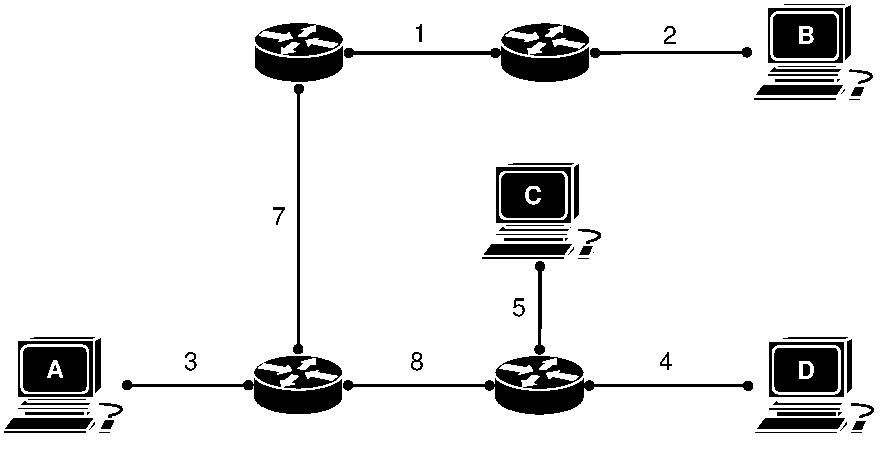
\includegraphics[scale=0.7]{img/pdf/example-physical.pdf}
\caption{Interconnection of nodes in the physical level.}
\label{figure:phys}
\end{figure}

If these peers participate in an overlay network according to one of the setups
of Figure~\ref{figure:overlay-confs}, then users will experience different
performances. In the overlay depicted in Figure~\ref{figure:overlay-1}, the
message will traverse the following sequence of links in the physical layer
(marked with their costs): $3 \rightarrow 7 \rightarrow 1 \rightarrow 2
\rightarrow 2 \rightarrow 1 \rightarrow 7 \rightarrow 8 \rightarrow 5
\rightarrow 5 \rightarrow 4$. In the alternative overlay of
Figure~\ref{figure:overlay-2}, the path will be: $3 \rightarrow 8 \rightarrow
4$. The total cost of the first sequence is $45 ms$, while the second yields a
mere $15 ms$. Therefore, we can conclude that the second overlay is more
congruent with the underlying physical network than the first one and, thus, is
more efficient.

\begin{figure}[ht]
\centering
\subfigure[Nodes B and C have direct overlay connection.] {
  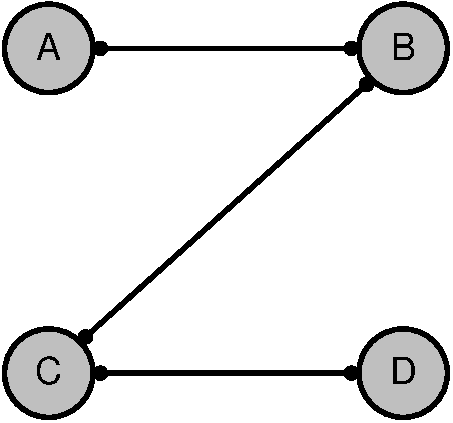
\includegraphics[scale=0.5]{img/pdf/example-overlay-inefficient.pdf}
  \label{figure:overlay-1}
}\qquad\qquad
\subfigure[Nodes A and D have direct overlay connection.] {
  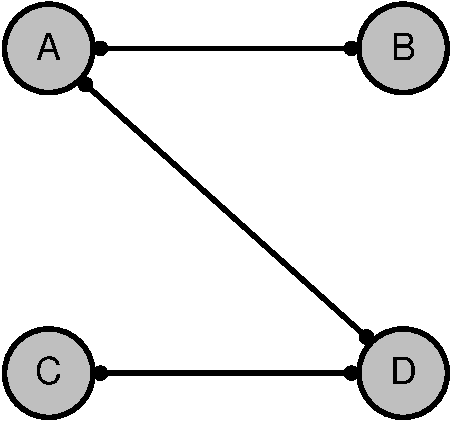
\includegraphics[scale=0.5]{img/pdf/example-overlay-efficient.pdf}
  \label{figure:overlay-2}
}
\caption{Two different overlay connection configuration.}
\label{figure:overlay-confs}
\end{figure}

Ideally, an overlay network should be constructed to achieve an optimal 
mapping among the overlay paths and the underlying network links to avoid
inefficient states were redundant physical resources are utilised for the
operation of a link on the overlay. The problem of constructing an optimal
overlay is referred to as the \emph{topology mismatch problem}, and is formally
defined as follows:
\begin{definition}
Let $V = \{v_1, ..., v_n\}$ be a set of points denoting the network nodes,
$\{v_i, v_j\} \in E$ be the set of unicast distances between nodes $v_i$ and
$v_j$, $G=(V,E)$ be a complete distance graph over $V$. The topology mismatch
problem is to construct a minimal spanning tree, where node degree is
restricted to a constant ($k\geq 2$) by the bandwidth of each node $v_i$.
\end{definition}

Early incarnations of the overlay protocols did not make use of the optimal
mapping with the underlying network topology. Gnutella, for example, is
considered far from scalable \cite{ritter_gnucantscale_2001} because every peer
chooses its neighbors in the overlay without any knowledge of the underlying
network, resulting in a mismatch between the two topologies. Queries may be
flooded over multiple paths merging in one peer while one of the paths would
have been enough. Moreover, peers may forward the same message to each other
before they receive the query messages from each other.
\cite{matei_mapgnutella_2002} showed that, even when 95\% of any two nodes are
less than 7 hops away from each other, a \emph{flooding-based} algorithm, like
the one used by Gnutella, can generate 330TB/month in a 50.000 node network. A
topology mismatch can thus have a serious effect on Internet router performance.

Similar problems are observed in decentralized structured schemes as well.
Typically, node IDs are assigned \emph{randomly}, resulting in excellent load
balancing, scalability, and robustness for the overlay. Unfortunately, this
randomness has a negative impact on the \emph{routing locality} of the network.
This means that even though the target node can be reached with logarithmic
overlay hops, the distance traveled in the underlying network, during the
overlay routing process, can be far from optimal.  The ratio of the actual IP
network distance a query travels to reach an object of interest (via overlay
routing) to the minimal IP network distance to that object (i.e. through IP) is
known as \emph{stretch} or \emph{Relative Delay Penalty (RDP)} \cite{CRZ2000}.

%%%%%%%%%%%%%%%%%%%%%%%%%%%%%%%%%%%%%%%%%%%%%%%%%%%%%%%%%%%%%%%%%%%%%%%%%%%%%%%%
%%%%%%%%%%%%%%%%%%%%%%%%%%%%%%%%%%%%%%%%%%%%%%%%%%%%%%%%%%%%%%%%%%%%%%%%%%%%%%%%
\subsection{Motivation and Goal for this Survey}
%%%%%%%%%%%%%%%%%%%%%%%%%%%%%%%%%%%%%%%%%%%%%%%%%%%%%%%%%%%%%%%%%%%%%%%%%%%%%%%%
%%%%%%%%%%%%%%%%%%%%%%%%%%%%%%%%%%%%%%%%%%%%%%%%%%%%%%%%%%%%%%%%%%%%%%%%%%%%%%%%
A topology unaware overlay network is able to control the sequence of peers a
message traverses before reaching its destination, but it is completely unaware
of how the actual packets are switched at the underlying infrastructure along
the overlay path. For example, a single logical point-to-point link on the
overlay typically corresponds to multiple physical links in the
underlying layer. Additionally, a link in the underlying network often lies
on several overlay paths causing increase of the traffic on the
link, known as the link's \emph{stress}~\cite{CRSZ2002}. Even in the case
of an approach that provides mechanisms to a new-coming node to detect close-by
peers at join time, the stochastic behavior with which peers join and leave
the overlay network, called the network's churn, further undermines the effort
for maintaining the best position in the network throughout the life-time of a
peer.

The topology mismatch problem is exacerbated by the extremely large amounts of
traffic generated by highly popular P2P applications (refer to the discussion
made in Section~\ref{section:intro}). Thus, solving the topology mismatch
problem is a fundamental challenge in contributing to the overall efficiency of
the Internet. Unfortunately, topology mismatch is known to be an NP-Hard problem
\cite{NPBOOK,C2000}. Adding to the complexity of the problem
is the fact that end-to-end latencies demonstrate \emph{triangle inequality
violations (TIVs)} which are a consequence of the Internet's structure and
routing policies and thus will remain a property of the Internet for the
foreseeable future \cite{zheng_irprtt_2005}. TIVs affect both network coordinate
\cite{cox_vivaldi_2004,wong_meridian_2005} and positioning \cite{ng_gnp_2001}
systems and makes the construction of IP-topology-aware overlays difficult.

Over the past several years, researchers have proposed and studied an extensive
array of heuristic solutions to the topology mismatch problem. The purpose of
this survey is to gather and organize the extensive knowledge that has been
produced. We hope to assist the reader to understand the different approaches
that have been proposed to tackle the topology mismatch problem. In order to do
so, we dedicate a discussion subsection after the presentation of the algorithms
for both unstructured and structured architectures. This section offers:
\begin{inparaenum}[\itshape i\upshape)]
  \item further discussion that can help the reader identify, through
a taxonomy, the pluses and minuses in the preceding material,
  \item a comprehensive tabular organization of the key-point information, and
  \item an attempt to give a pictorial comparison of the relative performance of
the algorithms.
\end{inparaenum}

In discussion we offer the reader a deeper insight for the observations that
pushed research toward some direction. Thus, we try to categorize these
approaches so that we can organize directions making them comprehensible
and helping the reader build critical thinking on the advantages and
disadvantages of each approach.

Tables provide a one-stop-shop overview for the algorithms so that can be a
helpful tool both as a companion during reading the survey and a reference for
future use.

Pictorial comparison consists of bar charts that give a relative feeling of the
performance of the various algorithms, discussed in the corresponding section,
in
terms of \emph{efficiency}, \emph{overhead} and \emph{scalability}; three
important characteristics for every distributed algorithm. For all we used a
coarse grained, three level, gradation to denote how well the algorithms do,
namely \emph{low}, \emph{medium} and \emph{high}. Each category has its own
interpretation of the above literal values. Efficiency means how well the
algorithm performs its search and topology adaptation functions, without
effecting other characteristics of the networks (e.g. BitTorrent's optimal
download performance). To name few, we assume that efficiency is
negatively effected when an algorithm reduces the search scope. Moreover, the
minimum-spanning-tree-based techniques have slow convergence speed in topology
adaptation or the high clustering impacts load balancing and constrains search
scope (or at least increases search satisfaction time), all reducing overall
efficiency. With overhead we track the cost to compute and communicate peer
join, message forwarding and topology maintenance. For example when exchanging
cost tables only along neighbors the traffic generated can be considered
trivial. Also duplicates minimization is a plus and lazy or heart-beat-based
overlay control mechanisms impose different amount of stress to the network.
Nevertheless, caching/replication helps reducing the overall overhead by
constraining the query from spreading too much. Low convergence speed of
minimum-spanning-tree-based approaches, we mentioned above for efficiency,
results also in additional computational and communicational overhead.
% TODO: We check
% complexity in the asymptotic sense, using \emph{Big O} notation % in order to
% check how the algorithm responds t. We take into account topology % creation and
% topology maintenance...
% TODO: HELP NEEDED!
With scalability we check the systems behavior with respect to the number of
participating peers. Low, medium and high scalability can be generally
considered in the order of hundreds, tenths of thousands and millions,
respectively. Fully distributed approaches is a plus (no system-centric entities
involved, no need for global knowledge) and topology adaptation strengthens
scalability in highly dynamic environments. Reduced search scope, on the other
hand, penalizes the scalability since the more peers coming in the network the
more potentially unsatisfied queries will there be. Furthermore, clock
synchronization is a limiting factor to scalability of a distributed system.

%
% TODO: SOME DISCUSSION FROM \cite{XTZ2003) CONTRADICTS TO THE
%TRIANGLE INEQUALITY ARGUMENT ABOVE
%
%[snip]
%Studies [14] have shown that triangle inequality may not hold in Internet
%topology. In fact, study from Pastry has shown that the proximity approximation
% is much worse when using the Mercator topology that is based on the real
% measurements of the Internet [3].
%



% \item Proximity Neighbour Selection\\
%Finally, the third approach, constructs the routing tables using proximity
%knowledge. Tapestry and Pastry's mechanisms of routing table
%maintenance try to minimize the distance to nodes appearing in a peer's routing
%table. Since routing is based on longest node ID prefix match, messages 
%are gradually forwarded to nearby nodes at each routing step.
%\cite{castro_proximityp2p_2002} argues on how Pastry exploits proximity
%neighbour selection in order to create a scheme that is (more) location-aware
%compared to the other well-known DHTs (CAN, Chord).
%
%\end{itemize}
%
%{\sethlcolor{yellow}\hl{
%HA: Possible criteria: based on which protocol (eg Gnutella, CAN etc), peer
%selection (topology selection, cluster, cache etc), supports dynamic update,
%runtimes}}
%%\textbf{Algorithm} & \textbf{Overlay structure} & \textbf{Forwarding} &
%\textbf{Cache} & \textbf{Overlay optimization} & \textbf{Proximity information}
%& \textbf{Base protocol} & \textbf{Dynamic update} & \textbf{Runtime} \\
%
%
%{\sethlcolor{yellow}\hl{
%HA: Possible criteria2: Overlay optimization structure, base protocol (eg
%Gnutella, CAN etc), dynamic update, runtimes, scalability}}
%
%{\sethlcolor{yellow}\hl{
%HA: maybe add also the year of publication, and see if there is a pattern in
%terms of the method and the year??}}

\section{Unstructured \p\ Networks}
\label{section:unstructured}

In this section, we present algorithms that tackle the topology mismatch
problem in unstructured \p\ networks. We classify them based on their
use of the overlay structure, their message forwarding scheme 
for peer communication and the techniques they use for detecting
proximity, to be used to optimize their overlay topology.

\subsection{Algorithms for Unstructured Architectures}

% TODO: READ A Near-Optimal Algorithm Attacking the Topology Mismatch Problem in Unstructured Peer-to-Peer Networks)

% BROADCAST OPTIMIZATION

%%%%%%%%%%%%%%%%%%%%%%%%%%%%%%%%%%%%%%%%%%%%%%%%%%%%%%%%%%%%%%%%%%%%%%%%%%%%%%%%
% \subsubsection{Improving search in peer-to-peer networks}

% \begin{figure}[ht]
% \centering
% \subfigure[Iterative deepening with three levels.] {
%   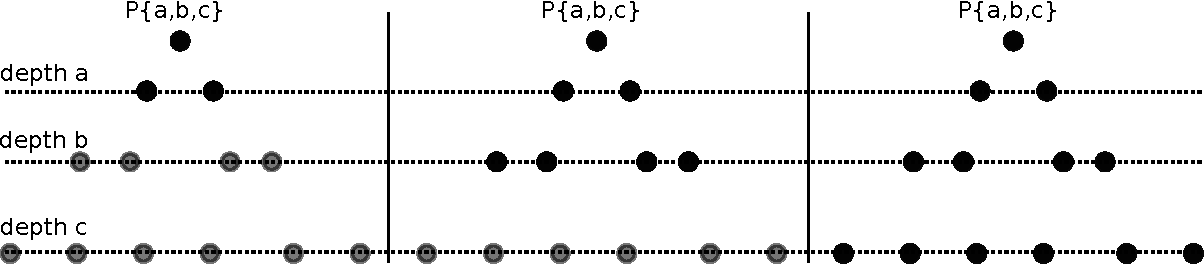
\includegraphics[scale=0.4]{img/algorithms/iterative_deepening}
%   \label{figure:dbfs:iterdeep}
% }\qquad\qquad
% \subfigure[Directed BFS.] {
%   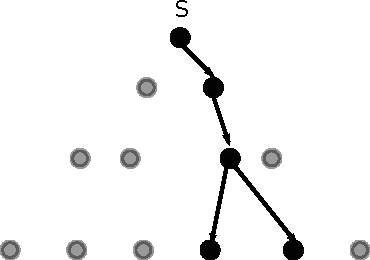
\includegraphics[scale=0.4]{img/algorithms/directed_bfs}
%   \label{figure:dbfs:dbfs}
% }\qquad\qquad
% \subfigure[Local indices with radius size equal to $2$.] {
%   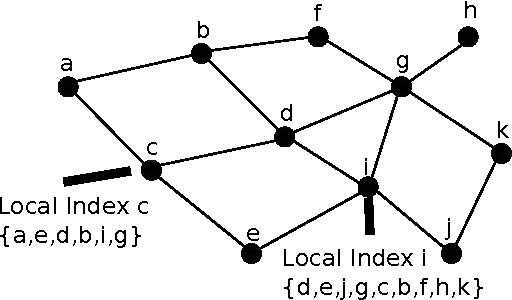
\includegraphics[scale=0.4]{img/algorithms/local_indices}
%   \label{figure:dbfs:localindx}
% }
% \caption{Improving search in P2P networks}
% \label{figure:dbfs}
% \end{figure}

To improve over {\sl Gnutella}'s ``blind flooding'' approach,
\cite{YG-M2002} proposed a practical and easy to implement solution 
weaved around three different message forwarding methods:
\emph{iterative deepening},
\emph{directed BFS}, and \emph{local indices}.

In \emph{iterative deepening}, 
%(see Figure~\ref{figure:dbfs:iterdeep})
the search is
performed on a BFS tree with multiple preset depths. 
The depth limit is iteratively increased by the source node for each query, 
based on the quality of the results. 
The source node may issue a new request with increased depth limit
that will trigger the nodes at the last depth level to resume the search. 
The iterative approach avoids restarting the entire search process 
from scratch at each iteration and reduces the load on the nodes of 
the upper levels of the tree. 
Its major drawback is the delay between successive iterations, as the
source-node has to examine the results at each attempt before deciding to
either quit or ``unfreeze'' the query.

The \emph{directed BFS}
tries to avoid the aforementioned delay by forwarding 
query messages only to a selected subset of available neighbors. The selection
criteria varies, from the number of results received previously or the distance
in terms of hops traveled to locate these results, to the bandwidth, or the
query load of the neighbor. That way, fewer nodes are visited but quality of
query responses is maintained, to a large degree, on the premise that the
selected heuristics can direct the search to the right path.
%
In \emph{local indices},
each node indexes data within a radius of $r$ hops and uses 
this local index to answer queries % on behalf of them 
without generating additional traffic. Local indices
greatly reduce the aggregate bandwidth usage of the network and 
improve query efficiency. However, updating such indices in 
the presence of frequent node joins/departures 
may introduce significant overhead should the radius is kept broad.
%%
Below, we outline how the techniques in~\cite{YG-M2002}
fare against the $3$ major performance criteria 
of Section~\ref{section:background}.
% \begin{center}
% \begin{tabular}{ccc}
% \textbf{Efficiency} & \textbf{Overhead} & \textbf{Scalability} \\
% \hline
% Iterative Deepening & ? & ? & ?
% Directed BFS & ? & ? & ?
% Local Indices & ? & ? & ?
% \end{tabular}
% \end{center}
\begin{center}
{\footnotesize
\begin{tabular}{rccc}
\multicolumn{1}{r}{} &
\multicolumn{1}{c}{\emph{Efficiency}} &
\multicolumn{1}{c}{\emph{Overhead}} &
\multicolumn{1}{c}{\emph{Scalability}}
\\
\cline{2-4}
\emph{Iterative Deepening} &
% needs recalculation in every iteration step
% extra delay imposed in a high churn environment that prohibits the algorithm
% to start from the last level of nodes and results in a restart of the whole
% process.
low &
% the process in not started from the beginning at each iteration step. For
% popular files this can substantially reduce overhead but for less popular
% ones, its performance might be uncertain due to the repeated restart of
% flooding
low &
% 
medium \\
\emph{Directed BFS} &
% Better time to satisfaction compared to iterative deepening
medium &
% Better quality and quicker results mean more aggregate bandwidth and
% processing power needs to be consumed since more nodes are involved (death
% spiral).
medium &
% BFS is Gnutella's non efficient communication method
medium \\
\emph{Local Indices} &
% efficiency is enhanced greatly since data pointers are replicated across the
% network
high &
% updating indices is a time and resource consuming process.
medium &
% the scalability is constrained by the indices update in a highly dynamic
% environment (high churn)
medium \\
\end{tabular}
}
\end{center}

%%%%%%%%%%%%%%%%%%%%%%%%%%%%%%%%%%%%%%%%%%%%%%%%%%%%%%%%%%%%%%%%%%%%%%%%%%%%%%%%
% \paragraph*{ \bf Delay Aware P2P System}
A \emph{delay--aware} \p\ system termed {\sl DAPS} 
was introduced in~\cite{ZL2005}.
{\sl DAPS}  seeks to attain reduced look-up times by dividing 
peer routing tables into several sectors of increasing delay. 
The source node that issues the query designates the delay 
boundary it may tolerate, providing so a \emph{pruning factor}.
In this context, user requests are forwarded only to 
nodes whose expected delay is less than or equal to the indicated boundary. 
{\sl DAPS} primarily focuses on user ``experience'' and deploys an
end-to-end delay monitoring mechanism that  may enable
the clustering of routing tables. 
In an dynamic environment, the formation 
of very accurate such routing tables might be however an elusive goal.
%With the clustered
%routing tables and the loose organization of DAPS' overlay network it is
%considered by is be tween structured and unstructured.
%%
In terms of the $3$ performance criteria, {\sl DAPS} stands as follows:
\begin{center}
{\footnotesize
\begin{tabular}{ccc}
\emph{Efficiency} & \emph{Overhead} & \emph{Scalability} \\
\hline
% Does not check for close by nodes, it just sorts the contents of a node's
% routing table.
% Also in a high churn environment a lot of time could be spend probing for
% distances, resorting routing tables and creating sectors. Moreover it just
% prunes distant neighbout
low &
% Sorting routing table entries is done locally so it is not affecting.
low &
%
medium
\end{tabular}
}
\end{center}

%%%%%%%%%%%%%%%%%%%%%%%%%%%%%%%%%%%%%%%%%%%%%%%%%%%%%%%%%%%%%%%%%%%%%%%%%%%%%%%%
% \subsubsection{Gia}

The key objective of the {\sl Gia} system~\cite{CRBLS2003} is 
to help alleviate the scalability omnipresent
in unstructured \p\ file-sharing systems.
At first, {\sl Gia} replaced {\sl Gnutella}'s blind flooding 
with random walks.
Although this adoption was 
a step in the right direction \cite{LCCLS2002},
issuing a single copy of the query within the network
effectively reduces the search scope and may negatively affect 
the success rate of the query in question.
To overcome this limitation, {\sl Gia} introduces
a token-based flow control mechanism 
that gradually redirects queries to nodes which are more
likely to answer. This flow control mechanism also helps prevent node
overloading as each peer ``announces'' the number of query requests it 
can handle, in terms of tokens, to its neighbors; to this end, 
peers only forward query requests to nodes that they previously
received tokens from. Further refinement to the search mechanism is the
support for \emph{one--hop replication} of pointers to content.
{\sl Gia} also acknowledges the heterogeneity in peer bandwidth,
processing power, disk speed, etc., of \p\ nodes and uses this
information when connecting nodes to each other.
By using a topology adaptation algorithm, 
{\sl Gia} places low capacity nodes within 
short proximity to peers with high performance features.
This topology adaptation algorithm is based on the metric 
each node maintains about its satisfaction --ranging between $0$ and $1$--
for the neighbors it finds itself associated with. 
Through message exchange, a peer can establish new connections 
or drop superseded ones in order to improve its satisfaction.
Despite the fact that {\sl Gia}'s topology adaptation algorithm 
that primarily focuses on the satisfaction of peers improves the network's 
scalability it falls short in addressing the mismatch problem
as considerations for the underlying network are not handled in explicit
terms \cite{LXLNZ2005}. Moreover it reduces the search scope, exhibits poor
performance in the worst case when matching data is not found quickly
\cite{PR2004,HJ2004} and can potentially build  disconnected topologies
\cite{MBL2006}.
%
In terms of the $3$ stated criteria, {\sl Gia}'s approach is as follows:
\begin{center}
{\footnotesize
\begin{tabular}{ccc}
\emph{Efficiency} & \emph{Overhead} & \emph{Scalability} \\
\hline
% Reduces the search scope.
medium &
% Only one copy of the query is issued to the network.
% A token based flow control mechanism redirects queries to nodes that are most
% likely to fulfill them.
low &
% Even thought the low overhead scalability is reduced by the reducing of
% search scope.
medium
\end{tabular}
}
\end{center}

%%%%%%%%%%%%%%%%%%%%%%%%%%%%%%%%%%%%%%%%%%%%%%%%%%%%%%%%%%%%%%%%%%%%%%%%%%%%%%%%
% \subsubsection{Distributed Cycle Minimization Protocol (DCMP)}
Another problem with topology unaware
systems is the duplication of messages due to cycles in the network graph.
Interestingly, such cycles appear even along the correct forwarding path.
\cite{ZKB2008} focuses on this exact deficiency of overlay networks and
introduces the \emph{Distributed Cycle Minimization Protocol
(DCMP)}, a dynamic, fully distributed method that removes cycles;
this is accomplished without sacrificing
overlay connectivity, resilience and other key properties of unstructured
\p\ architectures and by avoiding a hierarchical organization of peers. 
Once a cycle is detected in {\it DCMP}, the most powerful node in that cycle 
is elected as the \emph{Gate Peer} and the cycle is then broken in that place
that it will result in the minimization of the distance between the
\emph{Gate Peer} and all other nodes that are currently part of the cycle. 
This process is managed by using two specialized message types 
namely, \emph{Information Collection Message (ICM)} and \emph{Cut Message (CM)}. 
\emph{DCMP} bases its operation on messages whose travel is limited by an
imposed \emph{TTL} value (max set to $7$ for most cases). This inherently limits
the protocol in detecting cycles that span for more than \emph{TTL} nodes.
Even though cycle elimination does improve network performance, 
it cannot  directly contribute to the solution of the topology mismatch
problem, while its performance in a high traffic and churn environments and its
ability to retain important characteristics of a {\sl Gnutella}-like topology (i.e.,
like degree distribution, average peer distance, diameter e.t.c.) has been
doubted~\cite{CSG2010}. 
On the other hand, even though some of the overhead
saved by the duplicate message reduction is spent to control the cycle cutting
mechanism it is reported that still stays for example one to two orders of
magnitude less than LTM due to its ``lazy'' broadcasting of control messages
(as opposed to LTM's periodic approach) \cite{ZKB2008}.
%
%\begin{figure}
%\centering
%  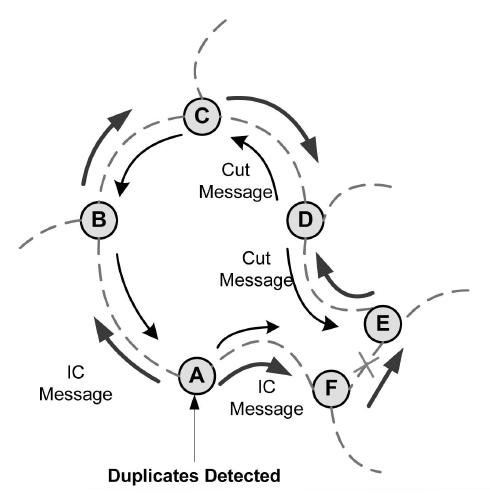
\includegraphics[scale=0.4]{img/dcmp.jpeg}
%\caption{Cycle elimination methods in DCMP}
%\label{figure:dcmp}
%\end{figure}
%
% TODO: SOME DISCUSSION
%Actually, the duplicate packet problem seems to hurt more the active nodes;
%those with higher capacities and bandwidth that contribute the most to the
%network.
The expected \emph{DCMP} behavior as far as our $3$ criteria is:
%
\begin{center}
{\footnotesize
\begin{tabular}{ccc}
\emph{Efficiency} & \emph{Overhead} & \emph{Scalability} \\
\hline
% It returns more result than LTM according to experiments in
% \cite{ZKB2008}
medium &
% Duplicates are an important fraction of the redundant overhead imposed by
% topology mismatch and thus DCMP minimizes this as possible.
low &
% fully distributed method
high
\end{tabular}
}
\end{center}

%       CACHING

%%%%%%%%%%%%%%%%%%%%%%%%%%%%%%%%%%%%%%%%%%%%%%%%%%%%%%%%%%%%%%%%%%%%%%%%%%%%%%%%
% \subsubsection{Replication Strategies in Unstructured Peer-to-Peer Networks}

In \cite{CS2002} and \cite{LCCLS2002}, replication is used as a way to improve
inefficient blind search. The observation is that as the number of replicas
increases in the network, it would be relatively easy to locate items even if
search is random.

The work discusses $3$ approaches for replication allocation namely \emph{uniform},
\emph{proportional}, and \emph{square-root replication}. In the uniform model,
all objects are replicated without taking into account the query distribution,
while in the proportional, objects are replicated analogously to their query
rate, so that frequently queried items can be found more often. Experimental
outcomes indicate that the uniform allocation minimizes the maximum search
length and so it can reduce the time spent on unsuccessful searches. The
proportional strategy effectively decreases the search time for popular items,
but suffers when needing to locate the rare entities. When it comes to expected
successful search size, it is the same for for both uniform and proportional
models and any approach in between to always behave much better. Finally, the
square-root model is an attempt to find the golden ratio between uniform and
proportional allocation models. It suggests setting the number of object
replicas to the square root of the searching rate for an object\footnote{An
interesting application of the square-root principle has also been explored
in the context of topology reconstruction, by ensuring node degree to be
proportional to the square-root of its content popularity \cite{C2005}.}.
Theory in \cite{CS2002} suggest that square-root minimizes the expected search size on
successful queries, claim that is supported by simulations \cite{LCCLS2002}.  

In \cite{LCCLS2002}, a \emph{k-walker} query algorithm is presented and shown
that using it along side square-root allocation results in performance similar to
{\sl Gnutella}'s query flooding method but incurring up to two
orders of magnitude less network traffic. Also checks $3$ strategies for
replica placement, namely \emph{owner replication} where an object is replicated
at the requesting node, \emph{path replication} that caches the object along the
path from the requesting to the providing node and \emph{random replication}
where the replication is taking place randomly on visited nodes. Observations in
this work are not directly applicable to structured DHTs, because it is assumed
that the lookup time for an object depends only on the number of replicas and
not the placement strategy \cite{RS2004}.

%%
%% SOME EXTRA DISCUSSION TAKEN FROM
%% IRM: Integrated File Replication and Consistency Maintenance in P2P Systems
%% 
%% Lv et al. [21] and Cohen and
%% Shenker [22] showed that replicating objects proportionally
%% to their popularity achieves optimal load balance but has
%% varied search latency, while uniform replication has the
%% same average search latency for all files but causes load
%% imbalance. Square-Root replication method replicating files
%% proportionally to the square root of their popularity is such
%% that both average search size and capacity utilization rate
%% vary per object, but the variance in utilization is consider-
%% ably smaller than with uniform replication, and the variance
%% in average search size is considerably smaller than with
%% proportional replication.
%%

The table below outlines how the $3$ allocation approaches fare:
%%
\begin{center}
{\footnotesize
\begin{tabular}{rccc}
\multicolumn{1}{r}{} &
\multicolumn{1}{c}{\emph{Efficiency}} &
\multicolumn{1}{c}{\emph{Overhead}} &
\multicolumn{1}{c}{\emph{Scalability}}
\\
\cline{2-4}
\emph{Uniform Replication} &
% Proportional and Uniform are the worst “reasonable” strategies
low &
% When item is created, replicate its key in a fixed number of hosts.
low &
%
medium \\
\emph{Proportional Replication} &
% Proportional and Uniform are the worst “reasonable” strategies
low &
% for each query, replicate the key in a fixed number of hosts (need to know or
% estimate the query rate)
medium &
%
low \\
\emph{Square Root Replication Allocation} &
% All (strictly) in-between strategies are (strictly) better than Uniform and
% Proportional - replication theory
medium &
% Assuming that each query keeps track of the search size then each time a query
% is finished the object is copied to a number of sites proportional to the
% number of probes that the search required.
medium &
% e.g. path replication is easy to scale, just detect the path along which the
% query ultimately got fulfilled
medium \\
\end{tabular}
}
\end{center}

%%%%%%%%%%%%%%%%%%%%%%%%%%%%%%%%%%%%%%%%%%%%%%%%%%%%%%%%%%%%%%%%%%%%%%%%%%%%%%%%
% \subsubsection{Tracing a large-scale Peer to Peer System: an hour in the life
% of Gnutella}
% TODO: This looks better as an analysis for the unstructured networks in
% general and specifically for caching, so it doesn't seem to contribute any
% new approach.... At least we do not present anything here. Maybe we need to
% revisit the paper itself once more
% \cite{Markatos02} analyses Gnutella network traffic traces and by concluding
% there is locality among query requests, proposes a caching algorithm that tries
% to exploit these findings . The analysis of the trace data reveals other
% important facts about the structure of the Gnutella network and the query data.
% One significant observation is that the geographic locations of clients do not
% have a correlation with the number of query requests they receive. This is an
% obvious result of the topology mismatch problem caused by the overlay structure
% of the Gnutella network. Gnutella's traffic is observed to be bursty both for
% query requests and query responses, even in longer intervals. It is observed
% that a peer receives 50 query messages per second on average! Moreover nine out
% of ten queries do not generate any response due to the inefficient design of
% the Gnutella network. When developing a caching system to exploit locality,
% applying an approach similar to web caching does not fit well with P2P systems.
% Caches in P2P systems not only have to consider the query string, but also
% the TTL value, the source of the query, and the time of the query as well.  In
% general, even though optimum caching is hard to achieve, it is reported that
% it improves the overall performance of the Gnutella network.

% \begin{center}
% \begin{tabular}{ccc}
% \emph{Efficiency} & \emph{Overhead} & \emph{Scalability} \\
% \hline
%
% ? &
%
% ? &
%
% ?
% \end{tabular}
% \end{center}


%       OVERLAY OPTIMIZATION

%%%%%%%%%%%%%%%%%%%%%%%%%%%%%%%%%%%%%%%%%%%%%%%%%%%%%%%%%%%%%%%%%%%%%%%%%%%%%%%%
% \subsubsection{Narada}

% \begin{figure}[ht]
% \centering
% \subfigure[Underlying network with edge costs.] {
%   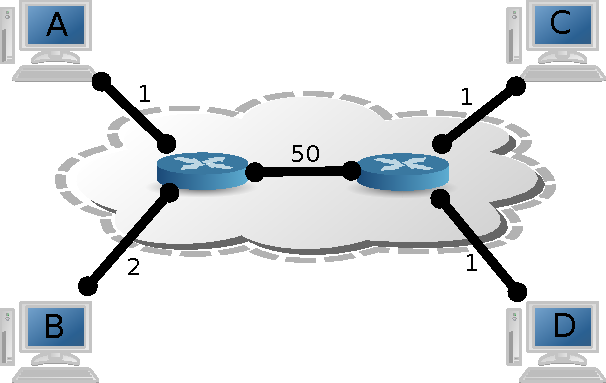
\includegraphics[scale=0.4]{img/algorithms/narada}
%   \label{figure:narada:underlying}
% }\qquad\qquad
% \subfigure[Peer A sends a message to the rest using regular broadcast.] {
%   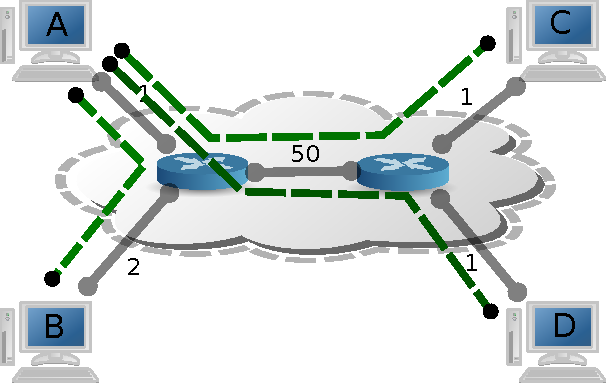
\includegraphics[scale=0.4]{img/algorithms/narada2}
%   \label{figure:narada:regu}
% }\qquad\qquad
% \subfigure[Peer A sends a message to the rest using end system multicast.] {
%   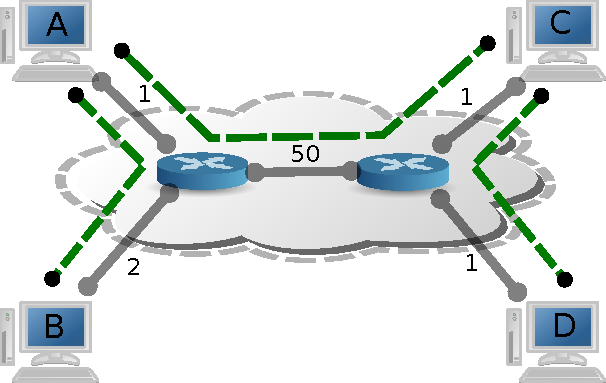
\includegraphics[scale=0.4]{img/algorithms/narada3}
%   \label{figure:narada:multicast}
% }
% \caption{A visualization of the Narada protocol.}
% \label{figure:narada}
% \end{figure}

{\sl Narada}~\cite{CRZ2000,CRSZ2001,CRSZ2002} is a generic
protocol for creating self-adapting overlay networks capable of 
application-layer multicast communications without requiring IP multicast
infrastructure at the network layer.
Although IP--multicast would present a choice in implementing
{\sl Narada}, it is in general considered that it violates the 
stateless design of the current Internet.
Despite the fact the {\sl Narada} was not designed as \p\ system per se,
it was the first (along with \emph{Scattercast} \cite{C2000}) to consider the
feasibility of overlay-based, application-layer services over the Internet while
taking into account bandwidth and latency properties of the underlying physical
infrastructure. In the context of this work, the inefficiency caused by the
topology mismatch and attempted to be tackled by building an highly connected
graph termed \emph{mesh}
with each source featuring its own minimum spanning tree. A gossip-protocol was
deployed for the creation of these spanning trees~\cite{LYL2008}.
%as shown in Figure~\ref{figure:narada}.
Both graph and trees are dynamically updated as nodes keep joining 
or departing the network. The protocol aims to ease the physical link stress,
the overall resource usage as well as the relative delay among end-systems. 
Unfortunately, the main limitation for {\sl Narada} is that 
although it works reasonably well for small groups, 
it does not scale well for larger networks. 
Hence, it is not a suitable choice for potentially large \p\ networks:
%%
\begin{center}
{\footnotesize
\begin{tabular}{ccc}
\emph{Efficiency} & \emph{Overhead} & \emph{Scalability} \\
\hline
%
medium &
% The overhead of Narada is proportional to the multicast group size
high &
% Maintaining the mesh for large multicast groups is expensive.
low
\end{tabular}
}
\end{center}

%%%%%%%%%%%%%%%%%%%%%%%%%%%%%%%%%%%%%%%%%%%%%%%%%%%%%%%%%%%%%%%%%%%%%%%%%%%%%%%%
% \subsubsection{Adaptive Overlay Topology Optimization (AOTO)}

Along with {\sl Narada}, the \emph{Adaptive Overlay Topology 
Optimization (AOTO)} \cite{LZXN2003} is one of the first attempts to address the
topology mismatch problem. \emph{AOTO} is a distributed algorithm that seeks to
optimize the usage of the underlying physical resources and operates in
$2$ phases:
\emph{Selective Flooding} and \emph{Active Topology}.
In \emph{Selective Flooding}, a minimum spanning tree is built for each peer and
its immediate neighbors so that queries do not flood the entire network and at
the same time preventing their search scope from shrinking. This way some
neighbors become non--flooding. During \emph{Active Topology}, each peer
replaces independently such non--flooding neighbors, with closer nodes as an attempt
to revise the overlay links so that they can reflect more closely the physical
network topology. Picking a replacement out of these non-flooding
neighbors follows a random policy called \emph{Randomized AT} algorithm.
To accomplish the above actions, a peer has to keep track of 
its communication costs with all its neighbors (e.g., network delays)
as well as the costs between any pair of neighbors. The \emph{randomized AT}
algorithm is applied by a source peer
every time its neighbor list is updated or an updated neighbor cost 
table is received.
%%
%\paragraph*{Selective Flooding (SF)}
%
% TODO: I DON'T REMEMBER WHY THE FOLLOWING IS MENTIONING LTM WHICH IS ANOTHER
%       ALGORITM. MAYBE THIS CAN BE USED AS A PART OF DISCUSSION AND/OR
%       COMPARISON OF AOTO AND LTM
% TODO: EDIT: LTM SEEMS A MISTAKE HERE BETTER NOT USE IT FOR DISCUSSION (THIS
%             IS AOTO)
%LTM's SF effectiveness has be proven to be detached from the different physical
% or overlay topologies. On the other hand, SF is more effective with large
%number of logical neighbors. It can reach an average optimization rate of 87.4
%percent on a logical topology with an average of 30 logical neighbors.
%
%\paragraph*{Active Topology (AT)}
%
%Different numbers of average logical neighbors has little to do with the
% effectiveness of AT. If the source has $n$ non-flooding peers, there are $n$
%potential neighbor replacements. The overhead to exhaust all $n$ possible
%replacements can be high, so in practice, after each replacement the source
%peer can decide whether it needs to find another candidate peer. This is done
%by computing the cost improvement ratio greater than some predefined
%termination threshold. The larger the threshold, the slower, in the number of
%optimization steps, the reduction of the normalized average distance. As a
%whole the average response time is significantly reduced when more optimization
%steps taken.
%%
\emph{AOTO}'s performance regarding the $3$ criteria is as follows:
%%
\begin{center}
{\footnotesize
\begin{tabular}{ccc}
\emph{Efficiency} & \emph{Overhead} & \emph{Scalability} \\
\hline
%
medium &
% tracking of communication costs to all peer's neighbors as well as between
% any pair of neighbors. Whenever a new neighbor cost table is received or
% there is a change of neighbors, the source peer has to re-calculate the
% multicast tree and apply the randomized AT algorithm.
high &
% needs global knowledge
medium
\end{tabular}
}
\end{center}

%%%%%%%%%%%%%%%%%%%%%%%%%%%%%%%%%%%%%%%%%%%%%%%%%%%%%%%%%%%%%%%%%%%%%%%%%%%%%%%%
% \subsubsection{Adaptive Connection Establishment (ACE)}
The \emph{Adaptive Connection Establishment (ACE)} 
approach~\cite{LZXN2004} uses the network delay as a metric 
to estimate the costs between nodes. Each peer computes the costs to its
logical one-hop neighbors and forms a \emph{neighbor cost table (NCT)} 
using a special routing message type. 
Any pair of neighboring peers exchange their \emph{NCT}s 
and so a minimal overlay topology can be formed. Based on the obtained
\emph{NCT}s a minimum spanning tree for each peer and its one-hop neighbors is
created. Finally, neighbors located physically far away 
are replaced by physically-closer counterparts. 
In particular, a peer $S$ iteratively probes the distance $d$ between
itself and every of its non-flooding neighbor nodes $G$ as well as
the distance between $S$ and $G$'s neighbors designated as $H$.
If $d_{SG} > d_{SH}$, then link $SG$ is replaced by link $SH$. If, on the other
hand, $d_{SG} < d_{SH}$ then also $d_{GH}$ and then we have the following
options. Either $d_{SH} < d_{GH}$ in which case link $SH$ is kept or
$d_{SH} > d_{GH}$ in which case $S$ will keep probing other $G$'s direct
neighbors.
%
The above optimization is conducted within $1$-neighbor
closure using as base, a peer and checking all its direct neighbors.
Evidently the scope of such an operation could be extended.
Should  a larger scope be used, a better topology matching can be obtained 
at a greater computational overhead.
%
% TODO: SOME DISCUSSION
%
%Simulations in \cite{liu_acesims_2004} show that the average scope of each
% query to cover the same scope of nodes is reduced by about 65 percent without
%losing any autonomy feature, while the average response time can be reduced by
%35 percent. Larger diameter topologies lead to better topology optimization
%rate but also to higher communication and computation overhead. It was also
%found that it is more effective in higher connectivity dense topologies.
%Compared to LTM, it comes short of convergence speed. In
%\cite{ni_mismatch_2004} shows reduction of both total traffic (90 percent) and
%response time (80 percent) to message queries without shrinking the search
%scope.Last but
%not least, it is concluded that work must be done on incorporating a more
%sophisticated selection policy for candidate non-flooding peers.
%

%In \emph{Adaptive Connection Establishment (ACE)} \cite{LZXN2004}, the
%authors extend the idea of AOTO by introducing optimizations based on the
%depths of the minimum spanning trees. But since the network delay is not
%always a reliable estimation method to detect the physical location of peers,
%the algorithm still suffers from the discrepancies caused by mis-located nodes.
%%
%%
\begin{center}
{\footnotesize
\begin{tabular}{ccc}
\emph{Efficiency} & \emph{Overhead} & \emph{Scalability} \\
\hline
% compared to LTM it has slow convergence speed because of the information
% exchange among each peer and all its neighbors.
medium &
% A little bit better that AOTO since the computation here is done within a
% certain diameter from the source peer
medium &
% Larger diameter topologies lead to better topology optimization
% rate but also to higher communication and computation overhead.
medium
\end{tabular}
}
\end{center}

%%%%%%%%%%%%%%%%%%%%%%%%%%%%%%%%%%%%%%%%%%%%%%%%%%%%%%%%%%%%%%%%%%%%%%%%%%%%%%%%
% \subsubsection{Location-aware Topology Matching (LTM)}

\emph{Location-aware Topology Matching (LTM)} \cite{LLXNZ2004}
seeks to optimize an overlay \p\ structure based on the physical topology.
To achieve this, peers issue special messages called
\textit{TTL-detector}s whose \emph{TTL} values are $0$ or $1$;
in this regard, peers 
discover $1$- and $2$-hop neighbor sets, designated as $N$ and $N^2$
respectively, and proceed to compute communication costs.
Time-stamps are used to derive network latency measurements that are then used 
to improve the overlay network without sacrificing the search scope.
Each node compares the latency information
received from its direct neighbors;
peers with longer latencies are placed on a
\emph{will-cut} list where they remain for a certain period of time 
after which they are finally eliminated 
and are placed on the peer's \emph{cut-list}. 
Thus, low-productivity connections are dropped and replaced by 
more efficient ones, reducing the
latency on the overall network. 
Although \emph{LTM} improves the overall efficiency of
the \p\ network, it is unable to offer any warranty for 
effectively addressing the mismatch problem.
%
% TODO: SOME DISCUSSION
%
%\paragraph*{Low productive connection cutting}
%There are three cases for any peer $P$ who receives $d(i, S, v)$ multiple
% times:
%\begin{inparaenum}[\itshape i\upshape)]
%  \item $P$ receives both $d(i, S, 1)$ and $d(i, S, 0)$
%  \item $P$ receives multiple $d(i, S, 0)$s from different paths, and P
% randomly chooses to process one
%  \item $P$ receives one $d(i, S, 1)$ and multiple $d(i, S, 0)$s, and $P$
% processes $d(i, S, 1)$ and one randomly selected $d(i, S, 0)$
%\end{inparaenum}
%If the link with the largest cost is found and is a direct neighbor then the
% connection is put in a will-cut list and stays there for a certain period of
%time. If it is not, then it is handled by other peers. After that period,
%connections are cut and recorded to $P$'s cut-list.
%
%\paragraph*{Source probing}
%For a peer $P\in(N^2(S) - N(S))$ who receives only one $d(i, S, 0)$, the cost
% of $PS$ is obtained (with list look-up or probing). Then $P$ compares it with
%the cost from each hop and if $PS$ has the largest cost, $P$ will not keep this
%connection, while otherwise the connection will be created.
%
%\paragraph{}
%Supposing $n$ is the number of peers, $c_n$ is the average number of neighbors
% and $c_e$ is the average cost of logical links, then in the flooding-based
%search the traffic incurred by one query from an arbitrary peer in a
%peer-to-peer network is $O(n)$. As observed in the Gnutella network
%\cite{sripanidkulchai_gnutella_2001}, each peer issues $0.3$ queries per minute
%in average, thus the per minute traffic incurred by the network with $n$ peers
%is $O(n^2)$. Because each $d(i, S, v)$ has a TTL of $2$ in each source peer,
%the traffic for one time LTM optimization in all peers is at most $2nc_n^2c_e$.
%If each peer uses LTM $k$ times per minute, the total traffic incurred is
%$2knc_n^2c_e$. Simulation shows the best value for $k$ is $2$ or $3$. So, the
%traffic overhead caused by LTM to the network is $O(n)$.
%
%TTLj-detectors, with $j > 2$, would detect and break cycles with more than 4
% links. LTM though, does not use such detectors because detector-flood traffic
%would increase significantly, and cut links between two end-peers, could cause
%queries initiated by them to traverse a path much more expensive than the cost
%on the the cut link.
%
%\paragraph{}
%LTM disadvantages are
%\begin{inparaenum}[\itshape i\upshape)]
%  \item disagreement of measured delay due to unsynchronized clocks causes
% problems when deciding the cut positions, which can influence the network
%connectivity, and
%  \item the network delay metric mainly focuses on disabling the connections
% between peers physically far away without considering the shortcuts created by
%powerful peers.
%\end{inparaenum}
%
\emph{LTM} fares as follows regarding our $3$  criteria:
\begin{center}
{\footnotesize
\begin{tabular}{ccc}
\emph{Efficiency} & \emph{Overhead} & \emph{Scalability} \\
\hline
% Authors claim 75% reduction on traffic cost and about 65% reduction on query
% response time.
medium &
%
medium &
%
medium
\end{tabular}
}
\end{center}

%%%%%%%%%%%%%%%%%%%%%%%%%%%%%%%%%%%%%%%%%%%%%%%%%%%%%%%%%%%%%%%%%%%%%%%%%%%%%%%%
% \subsubsection{Scalable Bipartite Overlay (SBO)}

The \emph{Scalable Bipartite Overlay (SBO)}~\cite{LXN2004,LXN2007} 
reduces the overhead of creating
and maintaining a minimum spanning tree 
by randomly dividing the nodes into
two groups --\emph{red}s and \emph{white}s-- 
and assigning different tasks to the two groups.
When a peer joins the network, it is randomly assigned with an initial
color (red or white).
Then the network bootstrap host node furnishes the joining peer with a list
of active peers along with their color information. 
The joining peer uses this list to 
establish connections to differently colored peers. 
In this regard, all peers form a a bipartite overlay. 
Using the network delay as a metric, white-peers 
peers measure distances from red counterparts
and report the encountered red neighbors.
Having information on all their $2$-hop neighbors 
($N^2$)
red-peers create minimum spanning trees for the neighbors in question and
assign efficient $2$-hop forwarding paths. This process can render a white
peer $E$ non--forwarding neighbor of the red peer $P$. Direct neighbor
replacement is a process conducted by $E$ in order to replace $P$ with a
$P' \in N^2(P)$ as its new neighbor. This adaptation tackles the
topology mismatch problem by reducing message duplication and shorten response
times caused by the problem identified as \emph{Revisit Not known (RN)}. RN is
the situation when a node is visited some times as a relay stop before it is
visited as an overlay peer, thus creating duplicate unnecessary messages to the
network and delaying query responses.
Even though this attempt is based on a simple and elegant solution it is
reported to not guarantee performance in terms of average communication delay
or search scope \cite{HLH2009}.
%
% TODO: SOME DISCUSSION
%
%In a static environment LTM may reduce traffic cost by around 80 to 85 percent
% while SBO reduces traffic cost between 85 and 90 percent. However, LTM  is
%proved to converge in around 2-3 steps while SBO needs 4-5 steps. Moreover LTM
%reduces response time by more than 60 percent in 3 steps while SBO needs 8. In
%a dynamic environment (10 minute average peer lifetime, 0.3 queries/sec by each
%peer) SBO and LTM reduce the average traffic cost per query (including the
%overhead due to the optimization steps) by 85 and 80 percent, respectively.
%Moreover LTM reduces the response time per query to 30 percent while SBO to 35
%percent.
%
% THE LINES BELOW NEED REWORDING
% ==============================
% \cite{LXN2004} Based on the above discussions, we can see the major
% advantages of using a bipartite overlay. First, the operation
% overhead is reduced. In ACE, every peer is required to
% probe the neighbor distance and compute the MST, whereas
% in SBO, white peers do the probing and red peers do the
% computing. Second, SBO extends ACE into two-hop
% neighbors, without additional information exchange
%
%\cite{ni_mismatch_2004} shows SBO, achieves approximately 85 percent reduction
% on traffic cost and about 60 percent reduction on query response time.
In regards to the $3$ stated criteria, \emph{SBO} behaves as follows:
\begin{center}
{\footnotesize
\begin{tabular}{ccc}
\emph{Efficiency} & \emph{Overhead} & \emph{Scalability} \\
\hline
% SBO reduces traffic cost between 85 and 90 percent
high &
% compared to LTM it has slower convergence speed thus incurs more, total,
% overhead.
medium &
%
medium
\end{tabular}
}
\end{center}

%%%%%%%%%%%%%%%%%%%%%%%%%%%%%%%%%%%%%%%%%%%%%%%%%%%%%%%%%%%%%%%%%%%%%%%%%%%%%%%%
% \subsubsection{Two-Hop-Away Neighbor Comparison and Selection (THANCS)}

The distributed heuristic termed 
\emph{Two-Hop-Away Neighbor Comparison and Selection (THANCS)}~\cite{LNXE2005,L2008}
attempts to minimize overlay hop costs.
\emph{THANCS} is essentially a \emph{local search method} as it aims 
to find a locally optimum solution by exploiting knowledge within 
a $2$-hop radius. The algorithm consists of two main components:
\emph{piggybacking neighbor distance on queries} and
\emph{neighbor comparison and selection}.

The \emph{piggybacking component} requires peers 
to probe immediate neighbors using delay distance measurements 
and store this information locally. 
The algorithm introduces a special query message type, 
the \emph{Piggy Message (PM)} which includes information about 
the neighbor identification (\emph{IP}) and measured distance ($d$). PMs are
piggybacked to normal
{\sl Gnutella} messages. 
When a node $P$ receives a query from $Q$, it constructs a
$PM_{PQ}$, piggybacks it to the query and forwards it to $P$'s neighbors. 
As soon as a neighbor detaches a received $PM_{PQ}$, records the distance 
$d_{PQ}$ and processes the query.
% When the neighbors receive it they detach the $PM_{PQ}$, 
% record the distance $d_{PQ}$ and process the query normaly. 
Selection of which incoming queries
should be piggybacked with a \emph{PM} is determined using either a
% proposed by either
\emph{pure probability-based (PPB)} or a \emph{new neighbor triggered (NNT)}
policy.


The \emph{neighbor comparison and selection} component defines that a peer $S$
probe all his $2$-hops away neighbors (a set denoted as $ N^2(S)$) not probed
thus far. Let $P$ be a $1$-hop distance neighbor of $S$, and $Q$ be a probed
peer by $S$. When $S$ receives a message piggybacked with message $PM_{PQ}$, 
% we identify the following cases.  %%AD put it passive as below.. 
the following $2$ cases are identified:

\begin{enumerate}
  \item If $Q$ is already a direct neighbor of $S$ then we check 
	the distances $d_{SQ}$, $d_{SP}$ and $d_{PQ}$. 
	If either $d_{SQ}$ or $d_{SP}$ is the longest, then the longest
  	link will be placed in a \emph{will-cut} list\footnote{A peer will not send or
  	forward queries to connections in its will-cut list but will preserve them
  	for some time in order not to effect ongoing response messages travelling the
  	inverse path.}. 
	If $d_{PQ}$ is the longest, then nothing is done by $S$; being
  	fully distributed, neighbor comparison and selection process, will have the
  	opportunity to handle $PQ$ link when initiated by peers $P$ or $Q$.

  \item If $Q$ is strictly a $2$-hop neighbor of $S$ and have never probed $Q$
  	in the past, stores distance $d_{SQ}$ and checks 
	distances $d_{SQ}$, $d_{SP}$ and $d_{PQ}$.
  	If $d_{SQ}$ is the longest, $S$ will not create link $SQ$. If $d_{SP}$ is the
  	longest, $SQ$ will be created and $SP$ will be put into the will-cut list.
  	If $PQ$ is the longest, links $SP$ and $SQ$ will be preserved expecting that
  	$P$ or $Q$ will disconnect $PQ$ later.
\end{enumerate}

%
% TODO: SOME DISCUSSION
%
% \begin{inparaenum}[\itshape i\upshape)]
%   \item is completely distributed and needs no global knowledge,
%   \item presents trivial overhead compared to the query cost savings
%   \item its convergent speed of the algorithm is fast enough (faster than
% minimum spanning tree approaches) so that is effective to dynamic
% environments, and
%   \item does not shrink the search scope.
% \end{inparaenum}
%
%In a static environment THANCS has been proven to be effective; optimizing 45
% percent out of the 60 percent of mismatched paths, constructing a nearly
%optimal overlay. This leads to a 60 percent reduction in traffic cost as well
%as a 40 percent decrease in query response time. In dynamic environments
%(Gnutella 0.6/Limewire super-peer-like and Ion flat-like), THANCS saves up to
%70 percent of the traffic cost in the super-peer topology and 55 percent for
%the flat one. Average response time is also decreased by 60 and 45 percent,
%respectively. Generally, THANCS has similar performance to LTM, without needing
%synchronization. SBO, incurring half the  overhead of AOTO, reduces the traffic
%cost the most, while THANCS has lower response time and converges faster than
%SBO. THANCS is, thus, more suitable for a more dynamic environment. In
%addition, THANCS is easy to implement and its operation overhead is trivial,
%compared with the other three approaches. This design, however, has the
%limitation of not being easily extend to also support non-flooding-based
%systems.

As discussed above, \emph{THANCS} is fully distributed and needs only minimum knowledge
of, at most, a $2$-hop distant peers. This features renders 
the method a good candidate for large overlay networks. 
Also its topology adaptation helps construct a well fit overlay
with respect to the underlying network--at least with respect to network
distances. In addition, will-cut list and distance caches (which store already
probed peers) minimize the unnecessary messages for the network maintenance.
%%
In \cite{HLY2010}, the simulation-derived results of \emph{THANCS} as far
average broadcast delay and overlay improvement guarantees are discussed;
overall, \emph{THANCS} fares as follows regarding the $3$ stated criteria:
%%AD rephrased more diplomatically the following as above.. 
% There are works in the literature though that criticize, through simulation
% results, the algorithm's average broadcast delay and overlay improvement
% guarantee \cite{HLY2010}.
% These characteristics are depicted to the $3$ evaluation criteria we use in this
% survey as follows:
%%%%%%%%%%%%%%%%%%%%%%
\begin{center}
{\footnotesize
\begin{tabular}{ccc}
\emph{Efficiency} & \emph{Overhead} & \emph{Scalability} \\
\hline
% 
medium &
% trivial overhead compared to the query cost savings and its convergent speed
% is faster than minimum spanning tree approaches so less overall overhead cost.
low &
% completely distributed and needs no global knowledge,
high
\end{tabular}
}
\end{center}

%%%%%%%%%%%%%%%%%%%%%%%%%%%%%%%%%%%%%%%%%%%%%%%%%%%%%%%%%%%%%%%%%%%%%%%%%%%%%%%%
The \emph{Hops Adaptive Neighbor Discovery (HAND)} algorithm~\cite{CLZHC2006}
uses a fully-distributed triple--hop adjustment strategy, applied to a network
graph $G$ in order to create an optimal graph $G^{*}$, free of the implications
of topology mismatch. This optimality is attained if all peer hop 
sequences $(v_1, v_2, \ldots, v_k)$ of $G$ exist in $G^{*}$ and are in the same
order. The latter indicates that in practice triple sequences $(v_1, v_2, v_3)$
are used. A mismatch is detected as follows: should we want to verify
a sequence, say $v_2-v_1-v_3$, two probing messages are dispatched from $v_1$ to
$v_2$ and $v_3$ and yield delays of $x$ and $z$ respectively.
%
When the probing message arrives at $v_2$, it gets forwarded
directly to $v_3$. 
Similarly, the message reaching $v_3$ is directly forwarded to $v_2$.
The above two forwarding actions seek to quantify 
the corresponding delays of $(v_2,v_3)$ and $(v_3,v_2)$ 
% physical paths denoted by $y$. 
for the physical path $y$.
%%AD check above... it is one path (not paths right?)
%%
If $y=z-x\pm\varepsilon$, the sequence $v_2-v_1-v_3$ is mismatched and should
be adjusted to $v_1-v_2-v_3$ by deleting edge $(v_1,v_3)$ and 
then adding a new $(v_2,v_3)$. 
If $y=x-z\pm\varepsilon$, sequence $v_2-v_1-v_3$ is mismatched and
should be adjusted to $v_1-v_3-v_2$ by deleting edge $(v_1,v_2)$ and adding a
new $(v_3,v_2)$. 
The  $\varepsilon$ is a small positive real number denoting
additional delays caused by possible forwarding and jitter delays. 
%%
The advantages of \emph{HAND} are that it
\begin{inparaenum}[\itshape i\upshape)]
  \item does not need any clock synchronization,
  \item is a fully distributed algorithm.
  \item involves low traffic overhead,
  \item can be used in dynamic \p\ environments, and 
  \item furnishes low query response times.
\end{inparaenum}
%
% TODO: SOME DISCUSSION
%
%Measurements conducted for evaluation purposes showed that in a static
% environment the algorithm can effectively decrease traffic cost by about 77
%percent and shorten the query response time by about 49 percent in less than
%two minutes. In a dynamic environment it shows similar behavior and with the
%size of the overlay network having little impact on the effectiveness of the
%algorithm. Compared to LTM both algorithms have almost the same traffic
%reduction rate, however on the response time reduction rate HAND has a higher
%one by about 4 percent. The traffic overhead of HAND is much less than that of
%LTM by an average of 55 percent.
In terms of the $3$ stated criteria, \emph{HAND} fares as follows:
\begin{center}
{\footnotesize
\begin{tabular}{ccc}
\emph{Efficiency} & \emph{Overhead} & \emph{Scalability} \\
\hline
% similar traffic reduction rate savings to LTM
medium &
% The traffic overhead of HAND is much less than that of LTM by an average of
% 55 percent.
low &
% no clock syncing needed, fully distributed and with low control overhead the
% algorithm can be considered scalable.
high
\end{tabular}
}
\end{center}

%%%%%%%%%%%%%%%%%%%%%%%%%%%%%%%%%%%%%%%%%%%%%%%%%%%%%%%%%%%%%%%%%%%%%%%%%%%%%%%%
% \subsubsection{Adaptive Peer Selection (APS)}
The \emph{Adaptive Peer Selection (APS)} approach uses 
machine learning techniques to form peer selection strategies based on past
experience~\cite{BFLZ2003}. A decision tree is used to rate peers based on
information collected for the characteristics of established connections. Such
features include connection link load, bandwidth, and past uploading experience.
Subsequently, a Markov decision process is used
% introduced as a mechanism 
to shape the policy for switching among the peers. The success of approach depends on
how fast the introduced peer selection functions. Admittedly, \emph{APS} is slow 
due its on-line learning process and inherent complexity \cite{ZZLZ2009}. 
\emph{APS}' behavior regarding the $3$ criteria has as follows:
% As far as the $3$ criteria is concerned, \emph{APS} has as follows:
\begin{center}
{\footnotesize
\begin{tabular}{ccc}
\emph{Efficiency} & \emph{Overhead} & \emph{Scalability} \\
\hline
% machine learning the best way to adapt the overlay 
high &
% high computation overhead for learning and very slow convergence speed for
% the learning process.
high &
% Complexity of computation, and slow convergence speed prevents the approach
% to scale, especially in high churn environments.
low
\end{tabular}
}
\end{center}

%%%%%%%%%%%%%%%%%%%%%%%%%%%%%%%%%%%%%%%%%%%%%%%%%%%%%%%%%%%%%%%%%%%%%%%%%%%%%%%%
The \emph{Innocuous Topology Aware Overlay Construction (ITA)}
approach~\cite{PRFM2009} seeks to offer both an overlay formation approach and
an effective way to carry out searching. When constructing the overlay,
\emph{ITA} exploits the notion of \emph{short} and \emph{long} connections.
Should $N$ be the number of network peers,  $\alpha \leq 1 $ a system-wide magic
number and $x$ an $\alpha$-related latency threshold, the bootstrapping peer
randomly selects $\alpha \ast N$ ``close'' (latency below $x$) and 
$\left( 1 - \alpha \right) \ast N$ distant (latency above $x$) nodes
as its neighbors.
%%QUE how do they select all these magic constants???
%%ANS This α constant seems to be the percentage of close neighbors selected by
% a peer out of its total degree. Can't find the criterion with which it is
% chosen though. Maybe we can ask... Mema :)
Searching occurs in $2$ phases: in the initial, the querying node
floods its distant neighborhood  with \emph{TTL=1}.
Subsequently, peers receiving a query over a ``long link'' commence a 
local flood with \emph{TTL=ttl} where \emph{ttl} is system-defined.
%%QUE how are you supposed to define these parameters?? in a fixed manner??
%%
%%ANS Don't understand... the paper says that for increased awareness we need a
%% small α (page 7). But in the beginning they give that short links (close-by)
%% are given by α*Ν. I guess this gets smaller for smaller α.... Also on
%% page 7 they say they choose α to be 0.1, 0.05 and 0.033 and that
%% this equals to ``10, 20, 30 long and and the same number of short links''.
%% I don't understand how they deduce these numbers. Since short links is given
%% by α*Ν and long by (1-α)*Ν at least the numbers should be different from
%% short and long links...
The main objective of the overlay construction phase is to yield a network that
exhibits low clustering. In turn, this is a beneficial characteristic for
random graphs as it can lead to a larger coverage of peers and at the same time
help reduce duplication of messages travelling around the network. This
combination offers efficient lookups that pose minimal or no negative impact to
other mechanisms possibly employed by the \p\ systems (e.g., $1$-hop replication
or dynamic querying mechanisms). Experimental results in the same paper suggest
a $50$\% reduction in communication latency among peers by cutting off some $20$\%
of the \emph{IP}-level traffic generated.
%%
Regarding the $3$ criteria, \emph{ITA} is placed as follows:
%
\begin{center}
{\footnotesize
\begin{tabular}{ccc}
\emph{Efficiency} & \emph{Overhead} & \emph{Scalability} \\
\hline
% low clustering with larger coverage of peers with the same number of messages
% and reduced duplication.
medium &
% construction at peer join, while searching using local ``floods''
low &
% the selection of neighbors is done at join time. No overlay adaptation means
% low scalability in dynamic environments.
medium
\end{tabular}
}
\end{center}

%%%%%%%%%%%%%%%%%%%%%%%%%%%%%%%%%%%%%%%%%%%%%%%%%%%%%%%%%%%%%%%%%%%%%%%%%%%%%%%%
% \subsubsection{EGOIST}
\emph{EGOIST}~\cite{SLLBBR2008} is a set of algorithms used 
to construct and manage overlay networks. 
\emph{EGOIST} utilizes a selfish approach in the sense that every participating
peer continuously updates its neighbors so as to minimize the sum of distances
to all destinations under shortest-path routing. 
A newly arriving peer, randomly connects to an already participating 
node through a bootstrap server. Once connected, the peer starts receiving
information throughout the link-state mechanism and thus, after some time, 
it has a complete picture of the overlay graph. 
Then, the peer estimates the delay to all other nodes to
determine its potential neighbors and ultimately connects 
to the overlay using some policy; such a policy might be 
for example the minimization of the average delay to all its
neighbors. 
\emph{EGOIST} requires extensive resource usage to continuously
update the overlay connections for all nodes in the system. This needs
$O(n^2)$ measurements. 
Fortunately, each node does not need to do these
measurements for maintenance (monitoring and updating) with all other
participating nodes, but just with a number of $k<n$ nodes that it chooses to
establish links with. 
The latter yields a reduced $O(kn)$ time complexity for
maintenance while complexity $O(n^2)$ is required less frequently 
and only when nodes reevaluate their connections.
%
\emph{EGOIST} fares as follows:
% Regarding the $3$ criteria, \emph{EGOIST}'s behavior is as follows:
\begin{center}
{\footnotesize
\begin{tabular}{ccc}
\emph{Efficiency} & \emph{Overhead} & \emph{Scalability} \\
\hline
% peer neighborhood selected to minimize, for example, average delay
high &
% link state info (heartbeat) and delay estimation to all other nodes
% resulting to a complete picture of the overlay graph.
high &
% need global knowledge
low
\end{tabular}
}
\end{center}

%%%%%%%%%%%%%%%%%%%%%%%%%%%%%%%%%%%%%%%%%%%%%%%%%%%%%%%%%%%%%%%%%%%%%%%%%%%%%%%%
The main objective of the \emph{Biased Neighbor Selection (BNS)} 
approach~\cite{BCCMSBZ2006} is to 
strengthen {\sl BitTorrent}'s~\cite{c_bittorrent_2003} locality 
by carefully choosing most of the neighbors of a peer to come from 
the same \emph{ISP}, while simultaneously adhering to the near-optimal
download performance of the protocol.
%%
By and large, {\sl BitTorrent} deploys mechanisms that have proved
aggressive to \emph{ISP} networking and accounting as they function 
in a ``without-borders'' approach. 
The default {\sl BitTorrent} specification
designates $35$ connections for each peer regardless if such connections are
placed within or outside the borders of the \emph{ISP} that hosts the node.
%%
\emph{BNS} proposes that only $k$ out of these $35$ connections be
established with nodes beyond the {\it ISP}-borders;
the $k$ connections offer an extended and ``global'' view of 
the network at large and seek to strike a balance between 
the load imposed inside and outside the \emph{ISP}.
The latter refrains peers from exchanging traffic through
expensive network links should there exist alternative local connections
offering the required services. 
%%
\emph{BNS} is realized through 
\begin{inparaenum}[1)]
\item
the modification of the tracker so that 
\emph{ISP}-local resources are rapidly identified
\item
the use of \p--traffic--shaping devices on \emph{ISP} edge--routers. 
\end{inparaenum}
%%
In~\cite{BCCMSBZ2006}, a combination of 
biased neighbor selection along with bandwidth throttling
and caching techniques for near-optimal lookup results is proposed. 
The effectiveness of \emph{BNS} is debated 
in~\cite{RTLCGZ2010} where experimental results suggest that 
most peers in a swarm reside in different authonomous systems (\emph{AS}s).
%%AD AS = autonomous systems??? - put it so. First time discussed!
Consequently, clients frequently do not have enough peers to leverage
intra-\emph{AS} connections \cite{RTLCGZ2010}.
%%AD rephrased as above - what is AS??? Acronym... 
% On the other hand, the effectiveness of \emph{BNS}
% is arguable by other studies, whose
% experimental results suggest that most peers in a swarm reside in different ASs,
% thus a client in most of the cases does not have enough peers to leverage
% intra-AS connections \cite{RTLCGZ2010}. 
Moreover, \emph{BNS} deployment
requires knowledge of \emph{ISP} network mappings and awareness of possible
changes that occur in the infrastructure limiting its widespread adoption; the
following table qualitatively depicts the expected behavior of \emph{BNS}:
%%
\begin{center}
{\footnotesize
\begin{tabular}{ccc}
\emph{Efficiency} & \emph{Overhead} & \emph{Scalability} \\
\hline
% inter-ISP cost minimized while retaining the near optimal performance of
% BitTorrent download.
high &
% this info is taken at swarm join
low &
% trackers should maintain and update proximity info/proximity info is
% retrieved from special hardware.
medium
\end{tabular}
}
\end{center}

%%%%%%%%%%%%%%%%%%%%%%%%%%%%%%%%%%%%%%%%%%%%%%%%%%%%%%%%%%%%%%%%%%%%%%%%%%%%%%%%
\emph{Ono}~\cite{CB2008} is a protocol that helps contain
{\sl BitTorrent} traffic within individual \emph{ISP}s
and enhances the downloading rates by favoring connections
within the borders of a single autonomous system. Contrary to
\emph{BNS}~\cite{BCCMSBZ2006},
\emph{Oro} leads to improved performance 
without requiring any explicit cooperation between 
\emph{ISP} subscribers or any additional
infrastructure and network topology information.
\emph{Oro}'s selection approach is 
landmark-based and leverages existing {\sl CDN}-infrastructure 
for peer distance estimation. {\sl CDN}s already use both static (i.e.,
geographical, \emph{IP}-clustering) and dynamic (i.e., network delay measurement)
information for their replica selection. Thus, the algorithm leverages the
observation that peers that are redirected to a specific {\sl CDN} replica does not
only mean that these are close by this replica but to each other as well.
%%
The redirection behavior is modeled in terms of \emph{ratio map}, 
a vector of \emph{$<$replica-server,ratio$>$} tuples, where \emph{ratio} is
the percentage of times the {\sl CDN} redirects the peer 
to the specific \emph{replica-server}.
%%
The protocol's bootstrapping phase consists of the incoming peer performing
{\sl DNS} lookups to {\sl CDN}-names to build its redirection information.
%%
Initially, the {\sl DNS} polling interval is set to $30$ seconds 
and increases by $1$ minute every time redirection information 
to the {\sl CDN} remains unchanged after the lookup.
The {\sl DNS} polling interval is halved if pertinent 
redirection information has changed.
To avoid the bootstrapping phase when the \emph{ratio map} 
is sufficiently fresh, 
\emph{Oro} persists the map after the end of a {\sl BitTorrent} session.
%%
Experimentation with \emph{Oro} yields minimization of
inter-\emph{ISP} traffic costs and achieves near optimal performance 
of {\sl BitTorrent} download~\cite{BCCMSBZ2006}.
The \emph{ISP}-friendly design of \emph{Ono} however has been questioned when 
it comes to Internet-scale~\cite{PMJKA2009,LCLX2009,CLYSR2011};
its qualitative rating stands as follows:
%%AD rephrased as above...
% Even though the results in the paper claim minimization of inter-ISP traffic
% cost while enhancing the, already, near optimal performance of BitTorrent
% download, similar to \cite{BCCMSBZ2006}, this ISP-friendly design of \emph{Ono}
% is questioned, especially on a Internet-scale-basis \cite{PMJKA2009,LCLX2009,CLYSR2011}.
%%%%%%%%%%%%%%%%%%%%%%%%%%%%%%%%%%%%%%%%%%%%%%%%%%%%%
\begin{center}
{\footnotesize
\begin{tabular}{ccc}
\emph{Efficiency} & \emph{Overhead} & \emph{Scalability} \\
\hline
% Authors claim minimization of inter-ISP traffic cost while enhancing the,
% already, near optimal performance of BitTorrent download.
medium &
% periodic DNS lookups and CDN redirection imposes medium control overhead to
% the method.
medium &
% the use of CDNs make the approach not fully distributed thus less scalable
low
\end{tabular}
}
\end{center}

%%%%%%%%%%%%%%%%%%%%%%%%%%%%%%%%%%%%%%%%%%%%%%%%%%%%%%%%%%%%%%%%%%%%%%%%%%%%%%%%
% \subsubsection{Locality-Awareness in BitTorrent-like P2P Applications}
In~\cite{LCLX2009}, three techniques that 
``inject'' locality awareness in {\sl BitTorrent}-like applications are discussed.
The first \emph{macroscopic-level} technique
focuses on improving the neighbor selection process. 
When a peer asks a tracker to join, 
the later sorts its swarm peers according to
their hop-count distance from the requesting peer 
send out the top-$k$ list of nodes (e.g., $k$=$50$).
%%
The second technique, applied in an \emph{intermediate-level}, manipulates the
{\sl BitTorrent} chocking/unchocking mechanism. A peer unchockes its $4$
closest in terms of 
%%COMM-VM I put ``autonomous system'' back in again because in the context of this
% paper we are dealing on the number of AS crossings (one-hop = one AS crossing)
% until we reach a neighbor.
autonomous system hop-count interested neighbors. 
The same applies also when the peer turns to 
the seeding state;  this  \emph{intermediate-level} approach favors
least distance and is in contrast to the original {\sl BitTorrent} 
implementation which favors uploading speed.
%%
The last technique operates at 
a \emph{microscopic-level} and substitutes the rare-first chunk picking of the
original {\sl BitTorrent} protocol that picks the rarest of the available
chunks to download next, with a locality-first policy; this picks first the
chunck is located closer. 
%%AD check slight rewording above
The distance value of a chunk is computed as the mean
value of the distances of the peers that posses it.
Through experimentation on a real-world Internet topology simulated in
{\sf PlanetLab}, the locality-based approach achieves traffic optimization.
Nevertheless, it does not do that well when compared with the
random approach of the standard {\sl BitTorrent} protocol.

%%AD changed the wording - check.. 
All $3$ techniques in~\cite{LCLX2009} seek to harness 
% in exposing 
the locality of the basic functions of the
{\sl BitTorrent} protocol. 
Even though they do not restructure the network to map
better to the underlying infrastructure, they favor the intra-\emph{AS} 
over inter-\emph{AS} communications thus, reducing the overall communication cost.
Again, there is a trade-off between reducing inter-domain
traffic and fairness among peers in terms of the data the peers upload~\cite{LCLX2009};
as far as the $3$ criteria, the overall approach fares as follows:
%%
\begin{center}
{\footnotesize
\begin{tabular}{ccc}
\emph{Efficiency} & \emph{Overhead} & \emph{Scalability} \\
\hline
% minimization of inter-AS traffic but unfair among peers.
medium &
% info (AS hop distances) acquired at swarm join
low &
% does not result in a better map to the underlying topology, it just eases
% the implications of complete locality unawareness.
medium
\end{tabular}
}
\end{center}

%%%%%%%%%%%%%%%%%%%%%%%%%%%%%%%%%%%%%%%%%%%%%%%%%%%%%%%%%%%%%%%%%%%%%%%%%%%%%%%%
% \subsubsection{TopBT}
The key objective of \emph{TopBT}~\cite{RTLCGZ2010} is to enhance
proximity awareness in {\sl BitTorrent}
without the need of additional infrastructure. 
which \emph{TopBT} is built on the conjecture that
a good peer selection metric should take into account both the
downloading speed and the network topology. The metric proposed is defined as
the ratio of download to upload rate ${d}/{u}$
divided by either the link-level $l$ or the number of routing hops required $a$.
This metric should guarantee selection of peers with high download rate, low
reciprocal upload demand and decreased routing hops.
The above \emph{TopBT}-metric is applied in various
aspects of the original {\sl BitTorrent} protocol to ``inject'' topology
awareness for improved peer selection. 
%%
In an effort to essentially improve on the inherent topology mismatch problem,
\emph{TopBT} modifies: 
\begin{inparaenum}[1)]
\item the peer list the tracker returns when someone first tries
to connect to the swarm, 
\item the initial connection establishment, and 
\item the unchoking mechanism in the {\sl BitTorrent}.
\end{inparaenum}
\emph{TopBT}'s key feature is
that it does not need wide deployment.
% of its same types in order to see results. %%AD I do not get the second part of the sentence
% that it does not need wide deployment of its same types in order to see results.
It also supports both link-hop and \emph{AS}-hop metrics to identify proximity in
different levels.
%
%A peer that runs the TopBT protocol evaluates its neighbors by periodically
%emitting pings or trace-routes in order to unchock those peer that exhibit less
%hops to reach and higher download rates. \emph{Link-hops} are measured by using
%the TTL value that the originator receives as a response from the remote
%peer\footnote{Initial TTL values are known for the different operating systems
%(e.g. 64 for Linux or 128 for Windows NT/2000/XP) so the originator can
%calculate the hops using the value of the TTL on the response message it
%receives.}. Also the peer, when off-line, builds a table that maps IPs to
%\emph{AS-hops}, using BGP dumps.
%%
Through experimentation on hundreds of {\it PlanetLab} and residential hosts,
\emph{TopBT} offers more than $25\%$ traffic reduction and $15\%$ faster downloads
if compared with popular {\sl BitTorrent} implementations.
In reference to the stated $3$ criteria, \emph{TopBT} fares as follows:
\begin{center}
{\footnotesize
\begin{tabular}{ccc}
\emph{Efficiency} & \emph{Overhead} & \emph{Scalability} \\
\hline
% it takes into account both dl speed and network topology. The later though is
% rather coarse grained since it is taken into account on the AS level.
medium &
% the algorithm does not involve extensive calculations.
low &
% Does not need infrastructure and the calculations are distributed so it can
% scale
high
\end{tabular}
}
\end{center}

%%%%%%%%%%%%%%%%%%%%%%%%%%%%%%%%%%%%%%%%%%%%%%%%%%%%%%%%%%%%%%%%%%%%%%%%%%%%%%%%
% \subsubsection{Underlying Topology-Aware Peer Selection (UTAPS)}
The \emph{Underlying Topology-Aware Peer Selection (UTAPS)}~\cite{LCY2008}
presents an enhanced peer selection strategy. 
\emph{UTAPS} operates in two stages: in the first,
it collects information to develop a picture of the underlying topology 
and in the second, it proceeds to make the peer selection based on 
this knowledge. In the first stage, \emph{UTAPS} employs
network tomography, a technique that probes from a large network's 
endpoints to infer its internal characteristics~\cite{chny_tomography_2002}. 
%%
Upon arrival of a new peer, the tracker trace-routes 
it to obtain some basic knowledge 
including \emph{IP} address, routers involved, \emph{RTT} and number of 
hops traversed.
The more the peers in the swarm the better 
picture a tracker has for the underlying infrastructure.  
The tracker provides this information to the newcomer in the form
of the bootstrapping peer list. 
These newly joined peers traceroute the tracker
peer list themselves and return back to the tracker in order to further enhance
the tracker's view of the infrastructure.
%%
In the second stage, \emph{UTAPS} employs a set of heuristics
which target those peers that expose low \emph{RTT} and are found within
certain hop-counts away from
the routers observed during the initial traceroute.
Peers running \emph{UTAPS}
% It is reported in~\cite{LCY2008} that peers running \emph{UTAPS}
instead of the random peer selection, achieve better downloading rates
and at the same time offer reduced burden on the underlying \emph{ISP}s~\cite{LCY2008}. 
\emph{UTAPS} stands as follows in regard to the $3$ criteria:
%%
\begin{center}
{\footnotesize
\begin{tabular}{ccc}
\emph{Efficiency} & \emph{Overhead} & \emph{Scalability} \\
\hline
% coarse grained approach of the network tomography doesn't provide a detailed
% picture of the underlying network that the peers can then exploit
medium &
% trace-route and hop counts and calculation from both the tracker and the peers
% (the later for all peers in the bootstrapping list) increases the control
% overhead of the approach.
medium &
%
medium
\end{tabular}
}
\end{center}

%%%%%%%%%%%%%%%%%%%%%%%%%%%%%%%%%%%%%%%%%%%%%%%%%%%%%%%%%%%%%%%%%%%%%%%%%%%%%%%%
% \subsubsection{An Effective Network-Aware Peer Selection Algorithm in
% BitTorrent}
A clustering approach that differentiates peers encountered in a swarm
in those that are local, intra-\emph{ISP} and inter-\emph{ISP} is 
presented in~\cite{QLZG2009}.
The classification is carried with the help of the core routers used 
while peers communicate with the tracker. It is assumed that even though the
network may be highly volatile, these core routers are are usually more stable.
For this, a newly arriving
{\sl BitTorrent} peer, trace-routes the tracker and stores vectors containing
information like the \emph{IP} address and the hop number of a traced router, as well as the
link delay of the traced router and the previous hop along the trace-route path.
These vectors are reported to the tracker which uses
this information
to classify the router through a $k$-means classification algorithm, with $k = 3$. 
For peer selection, \cite{QLZG2009} proposes a biased approach 
where the tracker returns $c$ close peers 
and $d\;=\;N-c$ distant peers, where $N$ is the length of the returned list. 
In choosing $c$, the tracker employs an iterative search process
first in the peer's local neighborhood. If not sufficient number of 
peers are available there, the tracker goes to intra-\emph{ISP} 
and subsequently, if needed, to the inter-\emph{ISP} cluster. 
%%
Experimentation in a controlled environment indicates up to
5\% faster downloading times as well as up to 22\% reduction of 
the total cross-\emph{ISP} traffic.
This clustering approach fares as follows in regard 
to the $3$ criteria:
%%
\begin{center}
{\footnotesize
\begin{tabular}{ccc}
\emph{Efficiency} & \emph{Overhead} & \emph{Scalability} \\
\hline
% It incorporates clustering of peers to inter- and intra ISP which is a
% rather coarse grained method.
medium &
% only on peer arrival proximities to routers are estimated and sent to the
% tracker. Even though the tracker is backing the identification of a peer
% being close or distant the actual computation is done in a distributed manner
% thus not incurring too much additional controlling overhead.
medium &
% TODO: how intensive with regards to computing power is an on-line k-means
% (with k=3) classification???
% VM: do we have an idea?
medium
\end{tabular}
}
\end{center}

%%%%%%%%%%%%%%%%%%%%%%%%%%%%%%%%%%%%%%%%%%%%%%%%%%%%%%%%%%%%%%%%%%%%%%%%%%%%%%%%
% \subsubsection{Peer-exchange Routing Optimization Protocols (PROP)}
In~\cite{QCYCZ2007}, two 
\emph{Peer-exchange Routing Optimization Protocols (PROPs)} 
are introduced to help adjust the neighborhood graph of an overlay network
while aiming at reducing the network's overall link latency.
\emph{PROPs} are weaved around the concept of
``exchange'' of neighbors among peers; 
this is carried out so that participant node can collectively 
benefit from the attained reduction in network delays. 
%%
This ``collaboration'', is what differentiates this approach 
from others by allowing two peers to optimize
their neighborhood environment, than simply letting each node to ``selfishly''
choose its own strategy. 
%%
%%COMM--VM ADDING SOME OPERATIONAL DETAILS BELOW.
The \emph{PROPs} follow two phases: during the \emph{warm-up},
a node $u$ probes its neighbors to collect distance information. 
Subsequently, $u$ contacts, at a fixed time rate \emph{timer}, 
a random node $v$, $nhops$ away. % from it. 
New distance information is calculated independently 
by nodes $u$ and $v$, now for the
hypothetical state when the potential exchange would occur. 
If the benefit gained, in terms of reducing the average distance among the peers involved, is
above some predefined threshold then the exchange does occur.
Otherwise, no further action is taken. 
The second \emph{maintenance} phase
differs from the warm-up in that the probability
of peers to be probed and the \emph{timer} interval that this happens
now depends on past peer exchange results.

In the generic form of the \emph{PROP-G} protocol, a peer can exchange all of
its neighbors with those of another peer. This essentially results in the two
nodes exchanging positions so the topology and connectivity of the overlay is
not affected by the operation of the algorithm. The optimized version
\emph{PROP-O} permits peers to exchange selected sets of their neighbors. It is
not allowed to exchange neighbors along the path of the nodes that perform the
exchange in order to ensure that in the end of the process the peers will remain
connected. Additionally, the algorithm needs to preserve the characteristics of
the network (i.e., the graph remains connected, preserve the degree of the
nodes), so the exchange always involves equal number of neighbors.
%%
The following table depicts the \emph{PROP}s behavior 
regarding the stated criteria:
%%
\begin{center}
{\footnotesize
\begin{tabular}{rccc}
\multicolumn{1}{r}{} &
\multicolumn{1}{c}{\emph{Efficiency}} &
\multicolumn{1}{c}{\emph{Overhead}} &
\multicolumn{1}{c}{\emph{Scalability}}
\\
\cline{2-4}
\emph{PROP-G} &
% The authors show that an Internet-like underlying physical topology has much
% better performance
medium &
% Exchanging neighbors within a radius of 2 (TTL value) reduces stretch
% significantly, while keeping the additional overhead at reasonable levels
low &
% The effectiveness of the scheme is reduced while the system size becomes
% larger, but as the number grows, this reduction becomes smaller
medium \\
\emph{PROP-O} &
% The algorithm can better reclaim the heterogeneity of peers (those with faster
% response) to reduce the system's aggregate delay. 
medium &
% Same as above
medium &
% The queries are directed through fast nodes so it is important such nodes
% be part of the network
medium \\
\end{tabular}
}
\end{center}

% TODO: SOME DISCUSSION
% PROP-G can be applied to both structured and unstructured overlays.

%%%%%%%%%%%%%%%%%%%%%%%%%%%%%%%%%%%%%%%%%%%%%%%%%%%%%%%%%%%%%%%%%%%%%%%%%%%%%%%%
% \subsubsection{Resolving the Topology Mismatch Problem in Unstructured
% Peer-to-Peer Networks}
% TODO: to be reviewed

% In \cite{HLH2009}, Hsiao et al, claim to construct topology-aware
% unstructured overlays that \emph{guarantee} performance qualities in terms of
% \begin{inparaenum}[\itshape i\upshape)]
%   \item the expected communication latency among any two overlay peers
% regardless of the network size, and
%   \item the broadcasting scope of each participating peer
% \end{inparaenum}
% . The algorithm constructs an undirected graph $G = \left( V, E \right)$
% comprised by two subgraphs. The first, namely $G^{\left( red \right)} = \left(
% V^{\left( red \right)}, E^{\left( red \right)} \right)$ in the paper's context,
% includes all vertices of $G$ and ensures the connectivity of the graph by
% securing at least one path between any two nodes. In contrast, $G^{\left( blue
% \right)} = \left( V^{\left( blue \right)}, E^{\left( blue \right)} \right)$,
% contains those vertices of $G$ that have free edges to link to other nodes and
% because these are fully utilized, the following also stands $E = E^{\left( red
% \right)} \cup E^{\left( blue \right)}$. A joining peer $u$, partitions its
% neighbors into two subsets, the $B_u^{\left( red \right)}$ and $B_u^{\left(
% blue \right)}$. In order to populate the $B_u^{\left( red \right)}$ subset, peer
% $u$ samples peers uniformly and at random. Then, each of these selected peers
% discovers a routing path starting from itself towards the node with the smallest
% (or the largest) ID in the system.

% TODO: CHECK ONCE AGAIN
% \begin{center}
% \begin{tabular}{ccc}
% \emph{Efficiency} & \emph{Overhead} & \emph{Scalability} \\
% \hline
%
% ? &
%
% ? &
%
% ?
% \end{tabular}
% \end{center}

%%%%%%%%%%%%%%%%%%%%%%%%%%%%%%%%%%%%%%%%%%%%%%%%%%%%%%%%%%%%%%%%%%%%%%%%%%%%%%%%% 
% \subsubsection{Distributed Domain Name Order (DDNO)}
The \emph{Distributed Domain Name Order (DDNO)} approach~\cite{Z-YK2005} 
uses domain names to detect topologically-close nodes.
The fundamental assumption of the approach is the nodes found in 
the same domain are also topologically close.
%%
\emph{DDNO}'s outcome is a flat overlay topology which, with some adjustments, 
can be utilized in super-peer architectures as well. According to the algorithm,
half of the possible connections of a node are used to connect to local peers
(called \emph{sibling} connections) and rest are used to randomly
connect to the peers anywhere on the network (called \emph{random} connections).
The former ensure the reduction of long distance traveling for messages, while
the latter secure the connectivity of the structure and prevent network
partitioning.

%%AD slight rewording throughout...
Upon arrival, a peer $n$ asks a \emph{host-cache} to establish its
random connections. 
To identify its siblings, $n$ multicasts a specialized message $l$ 
to locate the right candidate(s).
Initially, the behavior of this message, is modeled as a random walker,
until $l$ reaches some peer $d$ capable to guide it through its next step.
This capability is enabled through a \emph{ZoneCache}, a data structure that
contains information for nodes accessible in an $r$-hop radius from $d$.
Ultimately $l$ will reach a node $m$ that is candidate to become $n$'s sibling. 
Then, $m$ issues a broadcast message to its own siblings and then all in the group will
inform the initiating peer $n$ of who is willing to accept new connections.
%%
The population as well as the maintenance of \emph{ZoneCaches} across the network
are key concerns when it comes to the efficient construction of the overlay.
While seeking to address the mismatch problem, 
\emph{DDNO} is a heuristic approach that uses
\emph{Split-Hash} and \emph{dnMatch} algorithms to effectively encode domain
names and determine domain locality respectively. 
In terms of our $3$ criteria, \emph{DDNO} fares are follows:
\begin{center}
{\footnotesize
\begin{tabular}{ccc}
\emph{Efficiency} & \emph{Overhead} & \emph{Scalability} \\
\hline
% Clustering approaches reduce search scope (or at least increase search
% satisfaction time). The algorithm tries to ease this problem by allowing some
% connections to be random
medium &
% overhead of split-hash and dnMatch is of low cost
% Walker message is multicasted only when sibling connections must be
% established.
low &
% it can be utilized in hierarchical architectures as well meaning increased
% scalability. Tests show that an increase from 5K- to 10K-node system slightly
% increases the average hops needed to satisfy a lookupDN message.
medium
\end{tabular}
}
\end{center}

%%%%%%%%%%%%%%%%%%%%%%%%%%%%%%%%%%%%%%%%%%%%%%%%%%%%%%%%%%%%%%%%%%%%%%%%%%%%%%%%
% \subsubsection{Critical Topology-Aware Grouping (CTAG)}
The \emph{Critical Topology-Aware Grouping (CTAG)} approach~\cite{ZL2006}
advocates a grouping strategy of peers based on the 
\emph{Internet Assigned Numbers Authority (IANA)} and 
the respective \emph{Regional Internet Registry (RIR)}'s \emph{IP} assignments.
%%
Based on these assignments, nodes that belong in the same 
organization are always addressed from the same block of \emph{IP} addresses.
\emph{CTAG}, exploits this observation to construct topology-aware unstructured
overlays. On top of this, \emph{Adjacency Measurement (AM)} is proposed, as
a technique which uses the longest matching \emph{IP} segment criterion to
compute node proximity. \emph{CTAG} focuses on both the construction of the
overlay as well as its constant and dynamic adaptation.
In its first phase, called \emph{bootstrapping grouping},
the {\sl Gnutella} web caching mechanism
is modified so that a newcomer may choose the closest, in terms of \emph{AM},
cache to retrieve its bootstrapping list. 
Similarly, during its second stage,
called \emph{dynamic revision}, the standard connection establishment mechanism
is also altered so that nodes with the highest \emph{AM} metric are chosen. 
When a node reaches its maximum number of neighbor
connections, it disconnects those neighbors with the lowest \emph{AM}.
\emph{CTAG} behaves as follows regarding the $3$ criteria:
\begin{center}
{\footnotesize
\begin{tabular}{ccc}
\emph{Efficiency} & \emph{Overhead} & \emph{Scalability} \\
\hline
% The technique partitions the system reducing the search efficiency
low &
% IP-based clustering involves low overhead
low &
% Has average scalability mainly to its low overhead. In larger applications the
% clustering of the system prevents the system from scaling smoothly.
medium
\end{tabular}
}
\end{center}

%###############################################################################
%###############################################################################
%###############################################################################
%       LANDMARKING
%###############################################################################
%###############################################################################
%###############################################################################


%%%%%%%%%%%%%%%%%%%%%%%%%%%%%%%%%%%%%%%%%%%%%%%%%%%%%%%%%%%%%%%%%%%%%%%%%%%%%%%%
% \subsubsection{Landmark Binning (LM)}\label{sec:landmark_binning}
% \begin{figure*}
% \centering
%   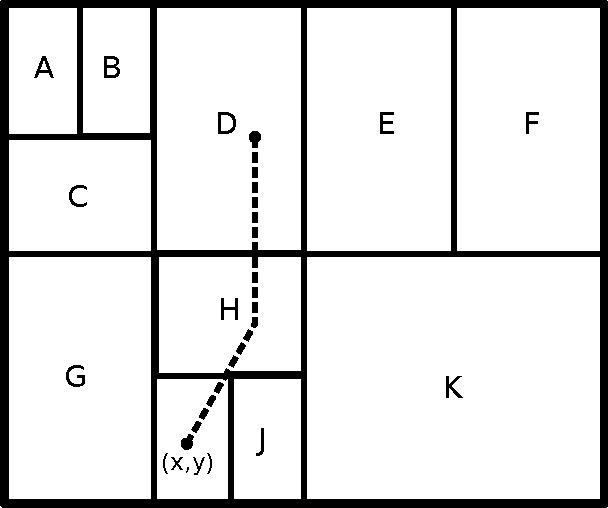
\includegraphics[scale=0.4]{img/algorithms/landmark_binning}
% \caption{Example 2D coordinate overlay and a sample routing path from node D to
% (x,y).}
% \label{fig:landmark_binning}
% \end{figure*}

\emph{Landmark Binning}~\cite{RHKS2002} partitions close-by nodes
into bins based on their distance from well known anchor nodes across the
Internet.%, as shown in Figure~\ref{fig:landmark_binning}.
To detect locality, peers mainly use network latency (i.e., \emph{RTT}).
%  as a measurement technique. 
Despite the fact that such delays are not always accurate,
they are used in~\cite{RHKS2002} for they are
non-intrusive, transparent and easy to apply.
%%
For the binning to work, a few anchor servers with known
physical locations need to be installed in strategic positions 
across the Internet. 
It is conjectured~\cite{RHKS2002} that $12$ such servers can prove
sufficient for the task.
An arriving node measures its distance from these landmarks
and unilaterally decides to join a specific bin based on its measurements.
Specifically, the node measures its round-trip time to each of the landmarks and
orders the resulting \emph{RTT}-values in a decreasing order. 
%%AD I do not understand what the following sentence says..
%%	for each peer there is a different bin right?
%
%The ordering represents a \emph{bin},
%in the sense of close-by nodes having the same landmark ordering and hence
%belong to the same bin. 
%
%% VM I CHANGED THE ABOVE AS BELOW TO REPHRASE IT.
Each permutation of the set of landmarks represents a specific bin. 
Should there $m$ landmarks be adopted, $m!$  different bins potentially exist. 
Peers that end up with the same ordering, belong to the same bin, in the sense that
if they experience similar overall latencies from fixed network points; it
is also  very likely that the peers in question are close to each other.
%%

As the operation of the method is independent of the model 
incorporated by the overlay network, the approach can be
applied with no significant changes to either
structured or unstructured \p\ systems.
%%
The rather obvious disadvantage of the approach lies in the
landmark servers that must be installed and maintained throughout the Internet.
Provided that a \p-system often may have a few million nodes 
connected at any given point in time, landmark servers do 
inherently play a pivotal role in the operation of the network. 
The approach has received a fair amount of criticism.
For instance, \cite{GSG2002} points out that end-hosts may bear the
cost of latency measurements and so, they may become bottlenecks.
\cite{CDCR2002,M2003,ZZZSZ2004}~argue that uneven distribution of nodes 
ultimately lead to load imbalances and \cite{RGJZ2004} indicates 
that its coarse-grained nature fails to
effectively distinguish among relatively close nodes.
Finally, \cite{XTZ2003} underscores the potentially increased maintenance cost(s).
%%AD rephrased what is below as above... The ONE sentence below cannot be read!!!!
%%%
% Moreover, studies like \cite{GSG2002}, pin point the fact that end-host shoulder the
% latency measurements as the scheme's scalability bottleneck while others argue
% about the uneven distribution of nodes potentially resulting in load imbalance
% \cite{CDCR2002,M2003,ZZZSZ2004}, its coarse-grained nature that fails to
% effectively distinguish among relatively close nodes \cite{RGJZ2004} and the
% potentially increased maintenance cost \cite{XTZ2003}.
%%%%%%%%%%%%%%%%%%%%%%%%%%%%%%%%%%%%%%
%%
%%
%
% Although latency estimation does not drain network resources,
% the scale of the approach does call for an alternative design.
% In this respect, \cite{RHKS2002} advocates the replacement of
% each landmark server by a cluster of servers.
% However, this approach may not entirely avoid the creation of 
% excessive network traffic flow through its landmark server-clusters.
%%
%%%%%%%%%%%%%%%%%%%%%%%%%%%%%%%%%%%%%%%%%%%%
%
%%
%To answer the question as to whether the algorithm actually contributes
% positively to the construction of an enhanced overlay, the paper defines the
%\emph{gain ratio} as the factor by which the latency reduces when someone
%communicates with a random node from the same bin than with one not in the bin.
%This is implemented with an inter-bin to an intra-bin latency ratio.
%
% TODO: LANDMARK BINNING FOR UNSTRUCTURED OVERLAYS
%
%For unstructured overlays the paper assumes \emph{a set of $n$ nodes where each
% node picks any $k$ neighbor nodes so that the average routing latency on the
%resultant overlay is low (assuming shortest path routing)}. According to the
%proposed heuristic algorithm called \emph{BinShort-Long}, a node picks its
%neighbors by choosing its $\frac{k}{2}$ closest\footnote{If the node's bin is
%not large enough for it to pick these $\frac{k}{2}$ neighbors, it picks the
%required nodes from the bin that matches the most in terms of landmark
%ordering.} ones (named \emph{short links}), using the \emph{binning} scheme and
%the rest $\frac{k}{2}$ randomly (\emph{long links}). The former set produces
%well-connected \emph{pockets} of nearby nodes while the later preserves the
%connectivity of the graph, both yielding a proximity factor of $\alpha = 0.5$
%in an attempt to preserve the beneficial properties of unstructured
%topologies\cite{merugu_str2unstr_2003}.
%
% TODO: SOME DISCUSSION
%
%A potential bottleneck could be the extra load that this
%``ping''-like scheme imposes to the landmarks, especially when we need instant
%reaction from our topology when dealing with the dynamic nature of the p2p
%networks.
%
%One disadvantage of this landmark scheme is related to the additional burden
% imposed to the landmark sites. The authors claim though that the algorithm
%requires so little work by the landmarks (maybe just echo to ping messages)
%that could in effect, act as ``unsuspecting participants''. Even if this is the
%case, the fact that it is not fully distributed, renders the protocol's
%scalability directly vulnerable to any system size increase as well as
%suitable for highly dynamic networks such as ad-hoc networks. Moreover, fixed
%points in a network are inherently more exposed to malicious attacks. The most
%significant downside of the algorithm though is that it can lead to an
%extremely uneven overlay ID distribution causing load unbalances and hot spots.
%Lastly, the scheme is coarse grained when it comes to distinguishing relatively
%close nodes\footnote{In the worst case, all nodes could ve clustered into a
%single bin.}.
%
%%
The landmark binning behaves as follows:
\begin{center}
{\footnotesize
\begin{tabular}{ccc}
\emph{Efficiency} & \emph{Overhead} & \emph{Scalability} \\
\hline
% The technique is coarse grained thus doesn't achieve optimal results
% (especially in small networks)
medium &
% The algorithm needs only nodes to compute distances to a small number of
% predefined nodes without exchanging any additional information.
low &
% The introduction of landmark servers renders the approach not fully
% decentralized, thus preventing it from scaling smoothly. Communicating
% and overloading landmark servers in high-churn systems is another scalability
% concern.
low
\end{tabular}
}
\end{center}

%%%%%%%%%%%%%%%%%%%%%%%%%%%%%%%%%%%%%%%%%%%%%%%%%%%%%%%%%%%%%%%%%%%%%%%%%%%%%%%%
% \subsubsection{mOverlay}
The \emph{mOverlay}~\cite{ZZZSZ2004} approach addresses scalability issues
that might arise when static landmark servers are in use.
To this end, the use of dynamic landmarks is proposed.
\emph{mOverlay}'s founding notion is that of a \emph{group} that 
designates a set of peers found in close proximity.
This proximity is user-defined in the protocol and 
may involve metrics including \emph{RTT}s and network latencies.
By and large a clustering approach, \emph{mOverlay} seeks to 
recreate small-world-like properties by producing a 
two-level hierarchical structure:
at the top level, there are only connections among groups 
while at the bottom, only \emph{intra-group} connections occur among peers.
%% 

Clearly, identifying groups and accurately finding the closest group 
to a peer is a fundamental concern in the creation of the overlay.
Nodes are grouped based on their distance to 
the groups already in the network, rendering
the latter be the \emph{dynamic landmarks} in the process. 
%%
For a incoming peer $Q$, 
the \emph{grouping criterion} designates that when the distance of $Q$ and
some group $A$’s neighbor groups is the same as the distance
between group $A$ and group $A$’s neighbor groups, then host $Q$
should belong to group $A$. 
During network initialization or when the grouping
criterion is not met, new groups are created.
A peer may reach its group by expending at most $O(logN)$ messages.
%%AD simplified sentence below as above...
% It is shown that in the proposed scheme, a new peer can 
% reach its group by expending at most $O(logN)$ messages
% within the network. 
Finally, \emph{mOverlay} maintains stability and constant 
overheads when a host either fails or departs the network;
this is achieved through periodic cache updates and group 
leader selections, should a node either leaves or dies.
%
%\paragraph{Locating process} A new coming host, $Q$, first connects to a
%globally known host cache called the \emph{rendezvous point (RP)} in order to
%retrieve the starting point in the overlay, say $A$ in group $1$. Host $Q$
%then, measures its distance to host $A$. At the same time, the later, sends
%information about the neighbor groups of group $1$ back to host $Q$. This list
%is called \emph{candidate group list}, and the new coming host sequentially
%measures its distance to each of them in seek for the closest one. If the
%\emph{grouping criterion} is met, host $Q$ belongs to group $1$. If not, a boot
%host from the closest group is found and the algorithm is re-run until the
%criterion is met or after a predefined number of repetitions. In the later
%case, $Q$ creates a new group comprising itself only. The above protocol does
%not favor hot-spots as it spreads the probability of visiting a group across
%the whole overlay and limits the overhead in the level of $O \left ( log N
%\right )$.
%
%\paragraph{General overlay operations} A set of additional protocols, are also
% introduced, similar to those found in traditional unstructured networks, but
%modified focusing on scalability and robustness. For example a protocol for
%\emph{group formation} is introduced that exploits the inherent characteristic
%of proximity, in the overlay, in order to efficiently detect the neighboring
%groups of a newly formed group from the set of adjacent groups of its closest
%neighbor. Additionally, during \emph{group joining} the corresponding protocol
%denotes the exchange of important information for group maintenance. This can
%be further improved by \emph{information sharing} between nodes of the same
%group, functionality handled by a dedicated flood-like protocol\footnote{Since
%nodes that belong to the same group are physically close this can be achieved
%at a minimum price.}. Moreover, another set of distributed protocols handle the
%\emph{information update}. The information that needs update, in the proposed
%architecture, is
%\begin{inparaenum}[\itshape i\upshape)]
%  \item the host cache, when a new node joins, and
%  \item the neighbors of groups, when a close-by group is generated.
%\end{inparaenum}
%Finally, in case of \emph{host failure} or \emph{host departure} the system is
% able to maintain its stability since there are defined operations for
%periodical host cache update and group leader selection if one leaves or dies.
%
%%
In terms of the stated $3$ criteria, \emph{mOverlay} fares as follows:
\begin{center}
{\footnotesize
\begin{tabular}{ccc}
\emph{Efficiency} & \emph{Overhead} & \emph{Scalability} \\
\hline
% The technique is coarse grained thus doesn't achieve optimal results
% (especially in small networks)
medium &
% The algorithm is iterative through the available groups. At each group
% probing of a candidate list must be performed. This process is done at
% bootstrapping time so the overhead increases in high-churn systems
medium &
% The introduction of dynamic landmark servers renders this approach much more
% scalable than the traditional static landmarking techniques 
medium
\end{tabular}
}
\end{center}

%%%%%%%%%%%%%%%%%%%%%%%%%%%%%%%%%%%%%%%%%%%%%%%%%%%%%%%%%%%%%%%%%%%%%%%%%%%%%%%%
%%%%%%%%%%%%%%%%%%%%%%%%%%%%%%%%%%%%%%%%%%%%%%%%%%%%%%%%%%%%%%%%%%%%%%%%%%%%%%%%
\subsection{Discussion on the Algorithms for Unstructured Architectures}
%%%%%%%%%%%%%%%%%%%%%%%%%%%%%%%%%%%%%%%%%%%%%%%%%%%%%%%%%%%%%%%%%%%%%%%%%%%%%%%%
%%%%%%%%%%%%%%%%%%%%%%%%%%%%%%%%%%%%%%%%%%%%%%%%%%%%%%%%%%%%%%%%%%%%%%%%%%%%%%%%




%%%%%%%%%%%%%%%%%%%%%%%%%%%%%%%%%%%%%%%%%%%%%%%%%%%%%%%%%%%%%%%%%%%%%%%%%%%%%%%%
%
% TODO: HOW CAN UNSTRUCTURED SCHEMES BE REFINED
%
%For this reasons, efforts have been placed for optimizing the efficiency of
%decentralized unstructured peer-to-peer networks. Research mainly focuses on
%\begin{inparaenum}[\itshape i\upshape)]
%  \item reducing unnecessary, redundant communication traffic, and
%  \item exploiting physical locality to reduce communication response.
%\end{inparaenum}
%The goal can be achieved at, both, the application-level network as well as the
%underlying physical one. In the first case by refining the message relay
%techniques, while in the second one, by adaptively reconstructing the
%application network to map as well as possible to the the physical network.
%
%%%%%%%%%%%%%%%%%%%%%%%%%%%%%%%%%%%%%%%%%%%%%%%%%%%%%%%%%%%%%%%%%%%%%%%%%%%%%%%%

While surveying efforts to overcome the mismatch problem
in the area of unstructured \p\ systems,
we came to identify four key methodologies 
utilized by the discussed approaches; they are:
\begin{enumerate}[\itshape i\upshape)]
  \item topology adaptation
  \item forwarding optimization
  \item caching and replication, and
  \item landmarking
\end{enumerate}
%
A key characteristic shared by many of the presented techniques 
is that they do not strictly adhere to a single methodology.
As discussed approaches attempt to address the inherently challenging problem 
of topology mismatch, they resort to heuristics and so, 
they do not often furnish ``pure'' solutions (i.e., solutions that exclusively belong to 
one of the $4$ aforementioned methodologies). 
%%AD rephrased as above..
% An important aspect of many implementations, is that since the above
% methodologies use heuristics to solve topology mismatch, an
% intrinsically difficult problem, no single approach can offer a robust solution.
% Thus, many of the algorithms we surveyed are actually combinations of multiple
% such methodologies, in an attempt to refine the results of using just a single one.
%%%%%%%%%%%%%%%%%%%%%%%%%%%%%%
For instance, \emph{mOverlay} combines topology adaptation with landmark binning 
while \emph{Gia} weaves together $3$ methodologies:  topology adaptation, 
forwarding optimization and caching. 
This combination inevitably leads to feature/performance trade-offs: for example, 
the effectiveness of a caching/replication component can be undermined
by a continuously adapting overlay that removes important links between peers.
If a technique is to be evaluated for a specific application domain,
its overall approach as well as its underlying used methodologies have to be considered.
%%AD rephrased as above... did not like much this "advised" - is not wrong BUT sounds funny
% For this reason, the reader is advised to critically approach either the overall
% algorithms or the separate methodologies when evaluating them for different
% application domains.
%%%%%%%%%%%%%%%%%%%%%%%%%%%%%%%%%%

Below, we outline how the proposed protocols use elements of the four
methodologies and we offer a summary qualitative comparison for all surveyed
approaches applicable for \emph{unstructured} \p \emph{systems}.
%%VM I brought the following paragraph here from the end of this subsection.
Moreover, Table~\ref{unstructured:table} offers a summary overview for each effort;
in particular, the Table shows which of the aforementioned methodologies 
every effort incorporates, the highlights of the effort as well as 
a rough estimation of the pros and cons of in its implementation.

%%%%%%%%%%%%%%%%%%%%%%%%%%%%%%%%%%%%%%%%%%%%%%%%%%%%%%%%%%%%%%%%%%%%%%%%%%%%%%%%
\subsubsection{Topology Adaptation Methodology}

Protocols based on topology adaptation 
modify the topology of the \p\ network
using various schemes. The two most commonly used
create \emph{spanning tree}s using connection graphs
as well as  \emph{clusters} of physically close nodes.

\emph{Narada} and subsequent algorithms including 
\emph{AOTO, LTM, SBO} try to solve the problem
by building ``a richer connected graph'' and by forming 
minimum spanning trees over
this graph that can efficiently route messages among peers. 
\emph{AOTO, LTM} and \emph{SBO} try to
overcome this limitation with ingenious schemes
like forming minimum spanning trees
for the $2$-hop away neighbors for each node, separating participant nodes into
groups, sometimes with different responsibilities and tasks at hand (e.g.,
\emph{SBO}). 
The advantage of building minimum spanning trees is that
they maintain the connectivity on the network in
an efficient manner while still preserving the overall search scope.
However, their construction and their update costs,
especially in dynamic and high-churn environments,
may cause large traffic overheads on the underlying
network~\cite{CRZ2000,CRSZ2001,CRSZ2002}.

The cluster-based approaches, on the other hand, 
link physically-close nodes to each other. 
\emph{T2MC}, for example, uses trace-route logs and 
\emph{DDNO} exploits domain names to cluster nodes in proximity at peer join.
Further enhancements may include dynamic local restructuring of the overlay
graph through neighbor exchange like in \emph{PROP} or cycle-cut like in
\emph{DCMP} to achieve continuous adaptation throughout a peer's life-cycle.
Unfortunately, commonly used methods for proximity detection across Internet do
not always return
reliable results and therefore, mapping accuracy is not guaranteed. Specifically
for traceroute, its overhead is not negligible and routers or firewalls in a
network may have already been configured to disable traceroute response from
the start. The most problematic aspect of clustering, though, is
its nature per se. 
Limited connectivity among the various local domains can
significantly shrink the search scope, negatively affecting the query response
time that the \p\ user experiences. Among others, \emph{DDNO} tries to 
balance the efficiency of the clustering approach 
with enhanced node connectivity by forcing half of each node's connections to be
with other, randomly selected, nodes.

As a methodology, topology adaptation, ultimately aims to reduce the 
average path traversing cost from one node to another.
In doing so, the methodology re-arranges the
overlay network so that it becomes a better fit 
for the underlying \emph{IP} network
as Figure~\ref{figure:topology-adaptation} depicts.
%%AD u always need a reference of a Figure in the text!!!
% as Figure~\ref{figure:topology-adaptation} depicts.
Despite the fact that the above is a plausible proposition,
it is not always advantageous though. For example, a topology adaptive
algorithm can exchange a slow edge in the overlay with a faster one
thus reducing the average latency of the network communication.
The pitfall here is that this new virtual link
can traverse a fast \emph{AS}--to--\emph{AS} link meaning that even though
message round-trip-time is reduced, it has actually additional cost in terms of
inter-ISP communication accounting and management.
%%
\begin{figure}[ht]
\centering
\subfigure[Inefficient overlay topology averaging $\simeq 16$ delay units.] {
  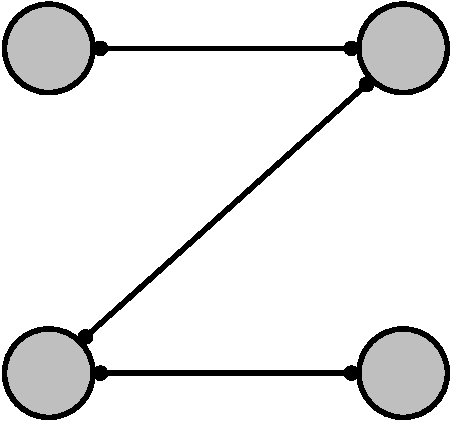
\includegraphics[scale=0.4]{img/pdf/topology-adaptation-before.pdf}
  \label{figure:topology-adaptation:before}
}\qquad\qquad
\subfigure[Efficient overlay topology after adaptation averaging $\simeq 11$ delay units.] {
  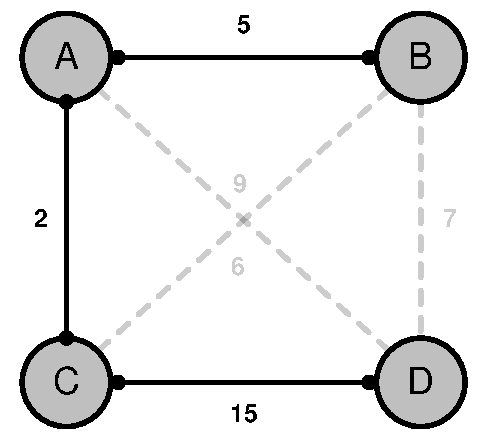
\includegraphics[scale=0.4]{img/pdf/topology-adaptation-after.pdf}
  \label{figure:topology-adaptation:after}
}
\caption{A simplified example on how overlay topology adaptation may improve matters.}
\label{figure:topology-adaptation}
\end{figure}
%%

%%%%%%%%%%%%%%%%%%%%%%%%%%%%%%%%%%%%%%%%%%%%%%%%%%%%%%%%%%%%%%%%%%%%%%%%%%%%%%%%
%%AD slight wording changes below - check
\subsubsection{Forwarding Optimization Methodology}
In unstructured systems, there is no way to know where data are actually located. 
This is why early works like Gnutella \cite{gnutellav04} used blind flooding, 
a \emph{BFS}--approach with depth $d$ and a system-maximum \emph{TTL} value 
(in terms of hops) for messages. 
This is inefficient since it generates a large number of
messages, a lot of which are duplicates. 
Approaches based on \emph{forwarding-optimization} propose 
intelligent search mechanisms in an attempt to
make searching more efficient.

Figure~\ref{figure:forwarding-optimisation} shows a simple example
of how forwarding optimization may work.
%%
\begin{figure}[ht]
\centering
\subfigure[Typical blind flooding.] {
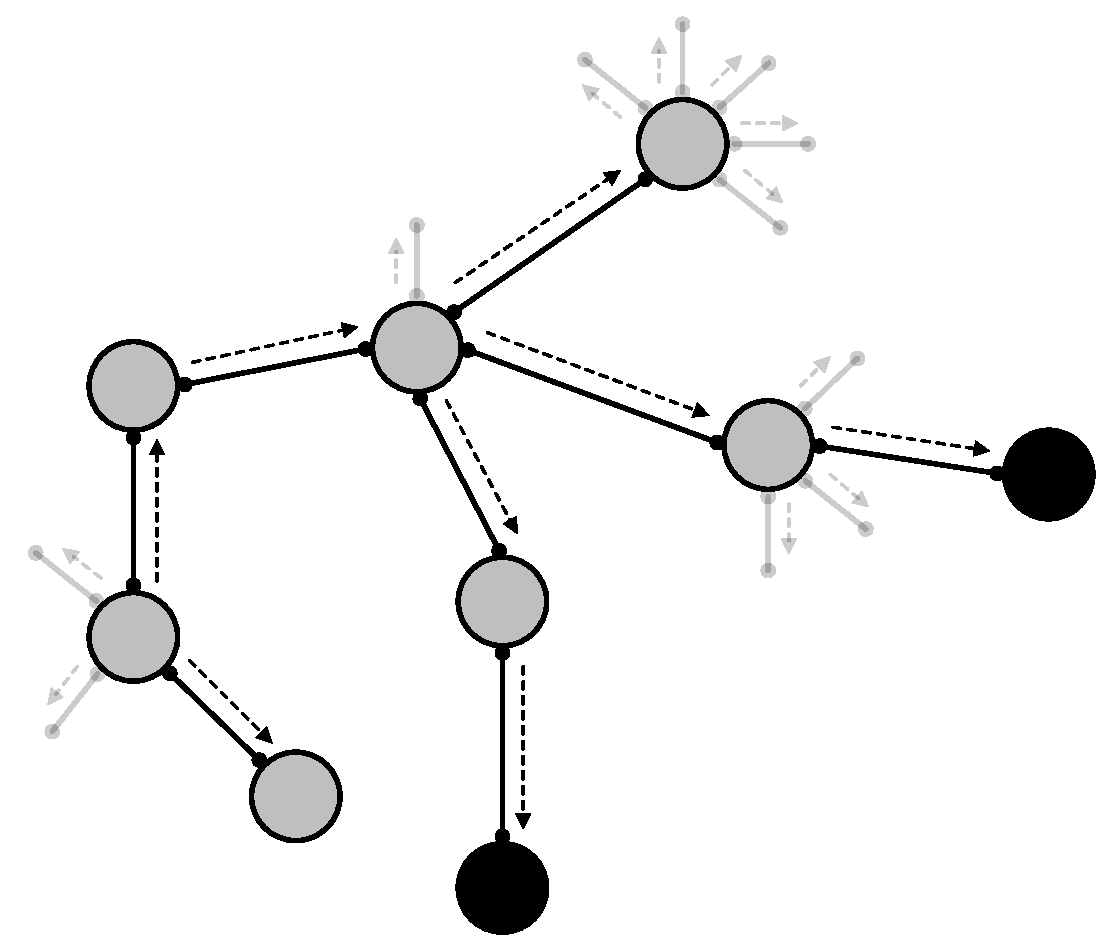
\includegraphics[scale=0.20]{img/pdf/forwarding-optimization-before.pdf}
  \label{figure:forwarding-optimisation:before}
}\qquad\qquad
\subfigure[A node can decide where to forward the messages.] {
  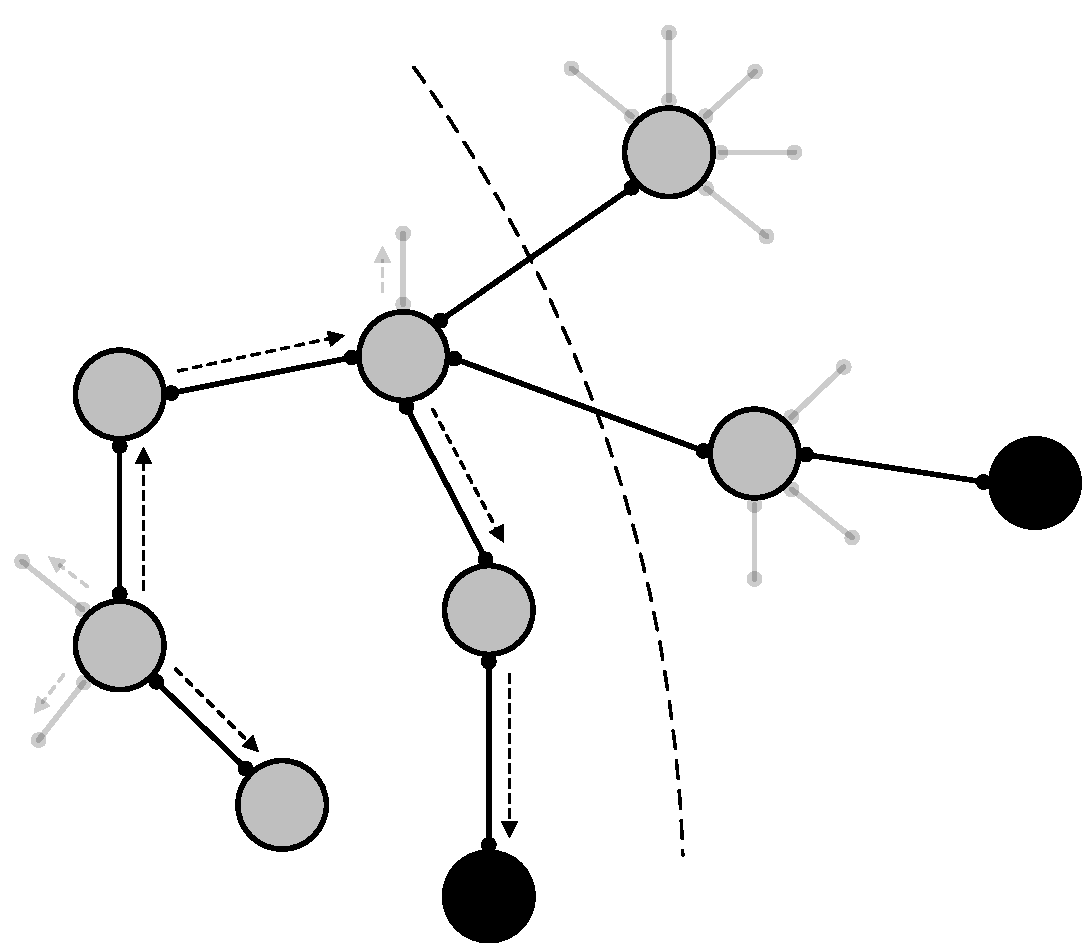
\includegraphics[scale=0.20]{img/pdf/forwarding-optimization-after.pdf}
  \label{figure:forwarding-optimisation:after}
}
\caption{Forwarding optimization in constraining message flooding.}
\label{figure:forwarding-optimisation}
\end{figure}
%%
Fig.~\ref{figure:forwarding-optimisation:before} 
shows a protocol that simply floods the entire network 
in search of object found in the nodes colored in black.
Alternatively, a node can decide to forward its
messages not to every output link but to a specific 
or subset of its outgoing links.
In Fig.~\ref{figure:forwarding-optimisation:after}, 
the node in the middle, does not flood its neighbors as instead 
in only picks one of them.
The dashed line on the right, shows that, 
for this routing process, the protocol has
rendered two potential forwarding paths as inefficient (e.g., the target nodes
show overloading signs).

Many alternative schemes have been proposed for this category, some of which we
have surveyed; iterative deepening, modified \emph{BFS}, local indices \cite{YG-M2002},
$k$-walker random walks \cite{LCCLS2002} or heterogeneity exploitation and
token-based flow control mechanisms \cite{CRBLS2003}. More sophisticated
alternatives also exist, taking into account application--level requirements
or even exploiting machine learning techniques to adjust overlay network
routing \cite{BFLZ2003}.

Forwarding-optimization schemes in unstructured \p\ systems can be classified
as \emph{DFS-} or \emph{BFS}-based. Routing indices \cite{CG-M2002} for example is a
\emph{DFS}-based technique while all the aforementioned are \emph{BFS}. Also,
the schemes in question can
be classified as deterministic or probabilistic (probabilistic, random or
ranking-based query forwarding). Iterative deepening and local indices
\cite{YG-M2002} are examples of deterministic approaches. Moreover, in the
literature algorithms are also taxonomised as blind or informed depending on
whether nodes keep some metadata to facilitate the search. For example,
$k$-walker random walks or iterative deepening are considered blind searches
while local indices informed.

On one hand, forward-optimization approaches have 
the advantage of enhancing the
search responsiveness and reducing the aggregate resource 
usage of the physical network. On the other, 
they suffer from drastic reduction of the search
scope (in Fig.~\ref{figure:forwarding-optimisation:after} the object on
the far right is not reached) thus, limiting the scalability of the whole
network. 
Forward-optimization suggestions address the problem of the mismatch 
in a limited manner since they do not provide any guarantees 
that overlay and underlying topologies are
aligned with each other.
%% let alone quantify the mismatch and try to alleviate.
%%AD I got the above out as superfluous
To this end, forward-optimization techniques are commonly applied in
conjunction with other methodologies to improve 
the overall quality of \p\ systems.


%%%%%%%%%%%%%%%%%%%%%%%%%%%%%%%%%%%%%%%%%%%%%%%%%%%%%%%%%%%%%%%%%%%%%%%%%%%%%%%%
\subsubsection{Caching and Replication Methodology}

Caching is widely used to exploit locality and minimize redundant
transfer of data. Caching has with much success been successfully 
adopted by web-- and file--server application environments. 
Since peers in a \p\ system also operate as servers,
it is intuitively expected that \p\ file--sharing systems can also benefit from
caching in improving performance and reducing overall resource usage. 
However, the design of caches in this context 
is non-trivial compared to the web-based caching. 
Due to the fact nodes play the double role of server and client,
two important issues have to be considered at design time. 
First, the lifetime of a query is short, as the nodes join 
and leave frequently. Second, the result
of a single query string is not always the same, as this depends on the
source of the query, the \emph{TTL} value set for the messages, 
the current interconnection of peers and the 
high volatility of the environment. 
Thus, to develop a successful caching system for a \p\ architecture, these
parameters also have to be carefully considered. 
\p\ caching/replication can be applied
at two different levels, namely caching indices or pointers to data 
(Fig.~\ref{figure:replication:index}) or caching the data itself 
(Fig.~\ref{figure:replication:data}). 
%%%
\begin{figure}[ht]
\centering
\subfigure[Indexing can reduce the cost of the last hop.] {
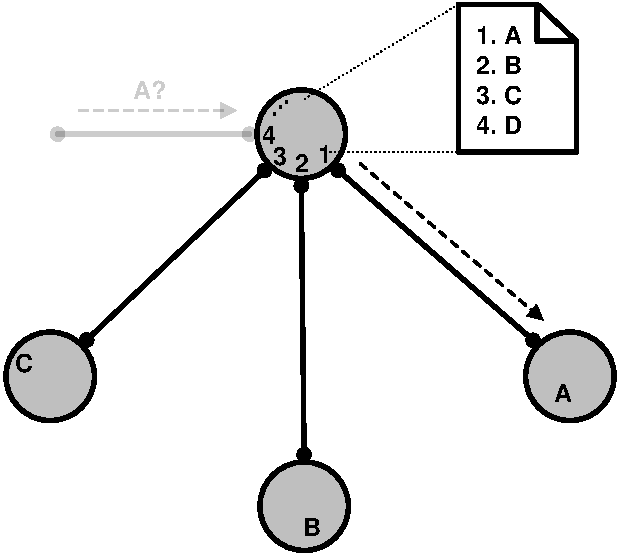
\includegraphics[scale=0.3]{img/pdf/replication-index.pdf}
  \label{figure:replication:index}
}\qquad\qquad
\subfigure[Data replication along the path of a successful query.] {
  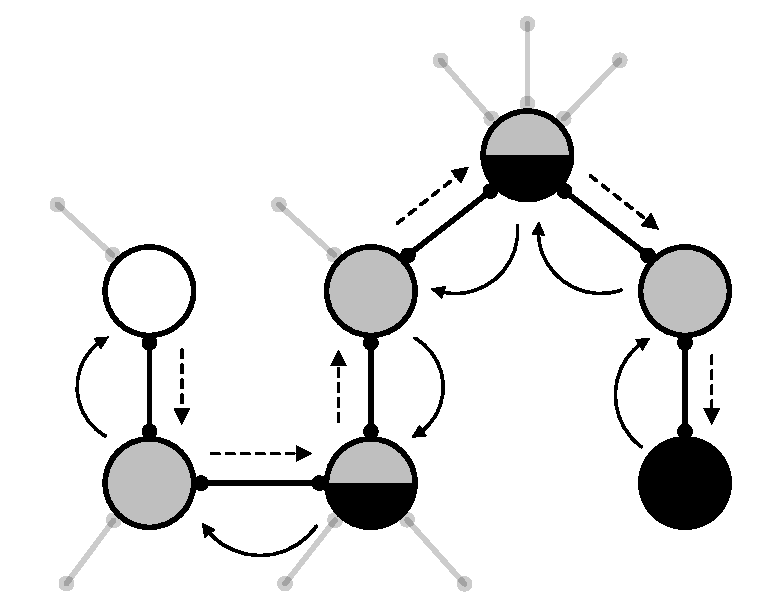
\includegraphics[scale=0.3]{img/pdf/replication-data.pdf}
  \label{figure:replication:data}
}
\caption{Index and data replication strategies.}
\label{figure:replication}
\end{figure}
%%
Successful implementations have
already been developed in some commercial \p\ systems, like 
\emph{KaZaA} or less popular ones including \emph{Gia} and \emph{BNS}.
%%%
Even though the state of the art in \p\ protocols using caching methods
helps reduce the burden of network resources, 
their contribution in addressing the actual mismatch between the overlay and
and the underlying networks remains limited.

% TODO SOME DISCUSSION
%The caching policy varies depending on the way protocol handles the
%index and the
%content. Centralized P2P systems
%use central index servers, while local caching systems, such as KazaA, use
%super peers
%to cache indices in a distributed way. Content caching is also possible in P2P
%systems, where nodes cache the forwarded content for further retrievals.
%Although caching has the above mentioned advantages,  duplication
%of messages still exist, which limits the scalability of these approaches.
%Therefore, cache based approaches are analyzed in the following categories:
%  \begin{itemize}
%    \item \emph{data index caching},
%    \item \emph{content index caching},
%    \item \emph{centralized}, and
%    \item \emph{local}.
%  \end{itemize}

%%%%%%%%%%%%%%%%%%%%%%%%%%%%%%%%%%%%%%%%%%%%%%%%%%%%%%%%%%%%%%%%%%%%%%%%%%%%%%%%
\subsubsection{Landmarking}\label{sec:landmark}

In landmark-based algorithms, nodes use network delay (e.g., \emph{RTT}) as a
distance measurement method to position themselves with respect to ``a priori''
known servers on the Internet, like \emph{Ono} which uses the \emph{CDN}-infrastructure
for this purpose.
These landmark--servers are used by nodes to estimate 
their positions based on the intuitive assumption that nodes
with similar distances to a set of landmarks, are physically close to each
other, as well, over the network. 
In Figure~\ref{figure:landmarking}, the newly
arriving peer, measures its distance to an array of landmark point denoted as
$L_n$ and and makes a sorted list of the peers, say in increasing order. Then in
order to choose the already participating peers with which to connect to,
the peer compares its list to the list of the potential neighbor. Peers with similar
measured distances to the these landmark points are likely to be close to
each other as well.
%%
\begin{figure}[ht]
\centering
  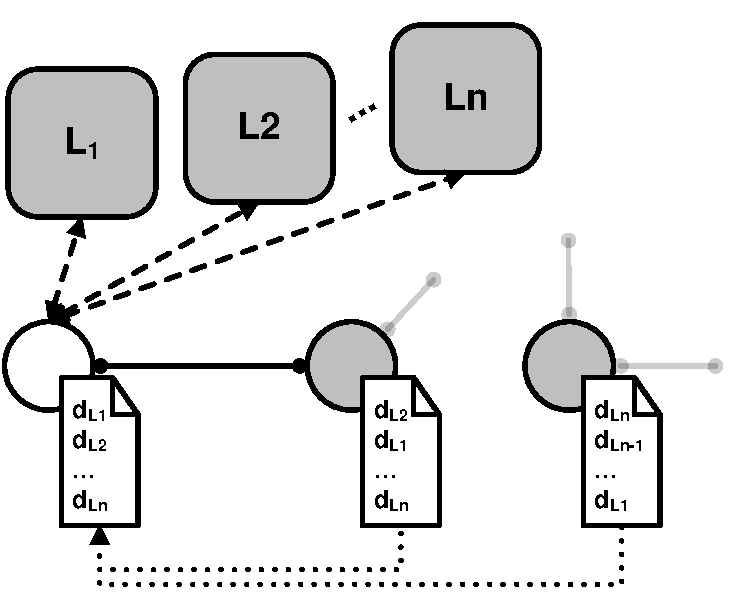
\includegraphics[scale=0.4]{img/pdf/landmarking.pdf}
\caption{Landmark binning during node bootstrap.}
\label{figure:landmarking}
\end{figure}

% Landmark--based protocols have four important drawbacks: First, the network
%%AD the correct here is "first" NOT "First"!
Landmark--based protocols have four important drawbacks: first, the network
delay is not a reliable distance estimation method. For example, based on the
load on the network, the delay to certain nodes or networks can significantly 
change over time; this eventually affects the distance measurements and yields wrong
measurements that ultimately lead to wrong estimated positions for the nodes 
or incorrect and non--optimal clusterings of nodes. 
Second, relying on predefined nodes
makes the whole paradigm not fully distributed and the landmark system prone to
single point of failure. Third, 
landmark infrastructure require costly installation and maintenance 
across the Internet and the different autonomous system domains. 
As popular \p\ file--sharing applications usually have millions
of peers connected to at any time, the network costs
of maintaining these landmark servers can be quite high. 
A possible solution to
the scalability problem of the static landmark servers is to use ordinary nodes
as dynamic landmarks in an approach reminiscent to that of \emph{mOverlay}.
% once they estimate their own positions. 
Even though this scales better, the accuracy of measurements
may affect the overall performance of the system. Moreover,it can
be characterized as a rather coarse-grained approximation, therefore not
particularly well suited for identifying the correct positions of nodes within
close distance to each other.
%%AD check the above made various small changes...

%%%%%%%%%%%%%%%%%%%%%%%%%%%%%%%%%%%%%%%%%%%%%%%%%%%%%%%%%%%%%%%%%%%%%%%%%%%%%%%%
%\renewcommand\arraystretch{1.9}% (MyValue=1.0 is for standard)

\begin{landscape}
%\begin{figure}[h!]
\hspace{-3ex}
\begin{center}
\footnotesize
%\begin{tabular}{
\begin{longtable}{
|m{2cm}
|m{1cm}
|m{1cm}
|m{1cm}
|m{1cm}
|m{3cm}
|m{5cm}
|
}
% |>{\columncolor[gray]{.7}}m{0.1\columnwidth}
% |>{\columncolor[gray]{.9}}m{0.1\columnwidth}
% |>{\columncolor[gray]{.8}}m{0.1\columnwidth}
% |>{\columncolor[gray]{.9}}m{0.1\columnwidth}
% |>{\columncolor[gray]{.9}}m{0.1\columnwidth}
% |>{\columncolor[gray]{.8}}m{0.1\columnwidth}
% |>{\columncolor[gray]{.9}}m{0.1\columnwidth}
% |}
\caption[Summary table for unstructured algorithms]{Summary table for unstructured algorithms.} \label{unstructured:table} \\
\hline
%%%%%%%%%%%%%%%%%%%%%%%%%%%%%%%%%%%%%%%%%%%%%%%%%%%%%%%%%%%%%%%%%%%%%%%%%%%%%%%%
% first head
\rowcolor[gray]{.5}
\textbf{Algorithm / Paper} &
\textbf{Topology Adaptation} &
\textbf{Forwarding Optimization} &
\textbf{Caching / Replication} &
\textbf{Landmarking} &
\textbf{Highlights} &
\textbf{Pros / Cons}\\
\hline
\endfirsthead
%%%%%%%%%%%%%%%%%%%%%%%%%%%%%%%%%%%%%%%%%%%%%%%%%%%%%%%%%%%%%%%%%%%%%%%%%%%%%%%%
% subsequent heads
\multicolumn{7}{c}%
{\tablename\ \thetable\ -- \textit{Continued from previous page}} \\
\hline
\rowcolor[gray]{.5}
\textbf{Algorithm / Paper} &
\textbf{Topology Adaptation} &
\textbf{Forwarding Optimization} &
\textbf{Caching / Replication} &
\textbf{Landmarking} &
\textbf{Highlights} &
\textbf{Pros / Cons}\\
\hline
\endhead
%%%%%%%%%%%%%%%%%%%%%%%%%%%%%%%%%%%%%%%%%%%%%%%%%%%%%%%%%%%%%%%%%%%%%%%%%%%%%%%%
% foot
\hline \multicolumn{7}{r}{\textit{Continued on next page}} \\
\endfoot
%%%%%%%%%%%%%%%%%%%%%%%%%%%%%%%%%%%%%%%%%%%%%%%%%%%%%%%%%%%%%%%%%%%%%%%%%%%%%%%%
% last foot
\hline
\endlastfoot
%%%%%%%%%%%%%%%%%%%%%%%%%%%%%%%%%%%%%%%%%%%%%%%%%%%%%%%%%%%%%%%%%%%%%%%%%%%%%%%%
% data
\textbf{\cite{YG-M2002}} &
{\large \Square} &
{\large \CheckedBox} &
{\large \CheckedBox} &
{\large \Square} &
\begin{tabular}[l]{m{3cm}}
Iterative Deepening (ID).\\
Directed BFS (DBFS).\\
Local Indices (LI).
\end{tabular} &
\begin{tabular}[l]{m{5cm}}
+ ID reduces the messages especially in upper levels of the tree.\\
%+ DBFS ??????\\
+ LI reduces aggregate bandwidth usage and improves query efficiency.\\
-- ID needs evaluation time between iterations.\\
-- DBFS uses heuristics so it depends on their efficient choice.\\
-- LI add index update overhead which might be heavy process especially in high-churn systems.
\end{tabular}
\\
\hline
%%%%%%%%%%%%%%%%%%%%%%%%%%%%%%%%%%%%%%%%%%%%%%%%%%%%%%%%%%%%%%%%%%%%%%%%%%%%%%%%
\textbf{DAPS \cite{ZL2005}} &
{\large \Square} &
{\large \Square} &
{\large \Square} &
{\large \Square} &
\begin{tabular}[l]{m{3cm}}
Clustered routing tables based on delay.\\
Pruning flood, an iterative deepening and multiple BFS approach with a pruning
boundary.
\end{tabular} &
+ It is a system between structured and unstructured.
\\
\hline
%%%%%%%%%%%%%%%%%%%%%%%%%%%%%%%%%%%%%%%%%%%%%%%%%%%%%%%%%%%%%%%%%%%%%%%%%%%%%%%%
\textbf{Gia \cite{CRBLS2003}} &
{\large \CheckedBox} &
{\large \CheckedBox} &
{\large \CheckedBox} &
{\large \Square} &
\begin{tabular}{m{3cm}}
Random Walks (RW).
\end{tabular} &
\begin{tabular}[l]{m{5cm}}
+ RWs issue one copy of the query thus not flooding the whole network.\\
-- RWs can reduce search scope.\\
\end{tabular}
\\
\hline
%%%%%%%%%%%%%%%%%%%%%%%%%%%%%%%%%%%%%%%%%%%%%%%%%%%%%%%%%%%%%%%%%%%%%%%%%%%%%%%%
\textbf{DCMP \cite{ZKB2008}} &
{\large \CheckedBox} &
{\large \Square} &
{\large \Square} &
{\large \Square} &
\begin{tabular}{m{3cm}}
Cycle detection.
\end{tabular} &
\begin{tabular}[l]{m{5cm}}
+ Drastically reduces duplicate messages.\\
-- Cannot detect cycles in distance bigger than the TTL value of the IC message.\\
\end{tabular}
\\
\hline
%%%%%%%%%%%%%%%%%%%%%%%%%%%%%%%%%%%%%%%%%%%%%%%%%%%%%%%%%%%%%%%%%%%%%%%%%%%%%%%%
\textbf{\cite{CS2002}} &
{\large \Square} &
{\large \Square} &
{\large \CheckedBox} &
{\large \Square} &
\begin{tabular}[l]{m{3cm}}
Uniform replication.\\
Proportional replication.\\
Square root replication allocation.
\end{tabular} &
\begin{tabular}[l]{m{5cm}}
+ Uniform replication reduces time spend on unsuccessful searches.\\
+ Reduces search time for frequent queries.\\
-- Proportional replication struggles in locating rare objects.
\end{tabular}
\\
\hline
%%%%%%%%%%%%%%%%%%%%%%%%%%%%%%%%%%%%%%%%%%%%%%%%%%%%%%%%%%%%%%%%%%%%%%%%%%%%%%%%
% \textbf{Tracing a large-scale Peer to Peer System: an hour in the life of Gnutella} &
% ? &
% ? &
% ? &
% ? &
% ? &
% ?
% \\
% \hline
%%%%%%%%%%%%%%%%%%%%%%%%%%%%%%%%%%%%%%%%%%%%%%%%%%%%%%%%%%%%%%%%%%%%%%%%%%%%%%%%
\textbf{Narada \cite{CRZ2000}} &
{\large \Square} &
{\large \CheckedBox} &
{\large \Square} &
{\large \Square} &
\begin{tabular}[l]{m{3cm}}
Mess creation.\\
Minimum spanning trees.
\end{tabular} &
\begin{tabular}[l]{m{5cm}}
+ Mess and trees are kept up to date in high churn environments.\\
-- Works well only for small groups of peers.
\end{tabular}
\\
\hline
%%%%%%%%%%%%%%%%%%%%%%%%%%%%%%%%%%%%%%%%%%%%%%%%%%%%%%%%%%%%%%%%%%%%%%%%%%%%%%%%
\textbf{AOTO \cite{LZXN2003}} &
{\large \CheckedBox} &
{\large \CheckedBox} &
{\large \Square} &
{\large \Square} &
\begin{tabular}[l]{m{3cm}}
Minimum spanning trees.\\
Peer proximity heuristic for removing costly links.
\end{tabular} &
\begin{tabular}[l]{m{5cm}}
+ Spanning trees only to immediate neighbors so no flooding and at the same time
no shrinked search scope.\\
+ Selective flooding effectiveness is detached from physical or overlay topologies.\\
+ The more logical neighbors, the more effective selective flooding becomes\\
-- High recalculation costs.\\
-- No sophisticated selection policy for candidate non-flooding peers.
\end{tabular}
\\
\hline
%%%%%%%%%%%%%%%%%%%%%%%%%%%%%%%%%%%%%%%%%%%%%%%%%%%%%%%%%%%%%%%%%%%%%%%%%%%%%%%%
\textbf{ACE \cite{LZXN2004}} &
{\large \CheckedBox} &
{\large \CheckedBox} &
{\large \Square} &
{\large \Square} &
\begin{tabular}[l]{m{3cm}}
Minimum spanning trees.\\
1-hop proximity heuristic.
\end{tabular} &
\begin{tabular}[l]{m{5cm}}
+ No flooding.\\
+ Less overhead compared to AOTO since computation is done within a certain diameter from the source peer.
-- Slow convergence speed.\\
-- Enhanced topology optimization comes to the expence of higher communication/computation overhead.
\end{tabular}
\\
\hline
%%%%%%%%%%%%%%%%%%%%%%%%%%%%%%%%%%%%%%%%%%%%%%%%%%%%%%%%%%%%%%%%%%%%%%%%%%%%%%%%
\textbf{LTM \cite{LLXNZ2004}} &
{\large \CheckedBox} &
{\large \Square} &
{\large \Square} &
{\large \Square} &
\begin{tabular}[l]{m{3cm}}
TTL detector (2-hop distance).\\
Delayed low productive connection cutting.
\end{tabular} &
\begin{tabular}[l]{m{5cm}}
+ Compared to AOTO, ACE and SBO achieves faster convergence speed.\\
-- Creates more overhead than AOTO, ACE and SBO.\\
-- Needs synchronization of peer clocks.\\
-- Does not consider shortcuts created by powerful peers when choosing to disable connections (only uses delay metric).
\end{tabular}
\\
\hline
%%%%%%%%%%%%%%%%%%%%%%%%%%%%%%%%%%%%%%%%%%%%%%%%%%%%%%%%%%%%%%%%%%%%%%%%%%%%%%%%
\textbf{SBO \cite{LXN2004}} &
{\large \CheckedBox} &
{\large \CheckedBox} &
{\large \Square} &
{\large \Square} &
\begin{tabular}{m{3cm}}
Red/white bipartite overlay.
\end{tabular} &
\begin{tabular}[l]{m{5cm}}
+ Efficient in both static and dynamic environments.\\
+ Compared to AOTO incurs half the overhead.\\
-- Needs almost double the steps of LTM to converge (static or dynamic environments).
\end{tabular}
\\
\hline
%%%%%%%%%%%%%%%%%%%%%%%%%%%%%%%%%%%%%%%%%%%%%%%%%%%%%%%%%%%%%%%%%%%%%%%%%%%%%%%%
\textbf{THANCS \cite{LNXE2005}} &
{\large \CheckedBox} &
{\large \CheckedBox} &
{\large \Square} &
{\large \Square} &
\begin{tabular}[l]{m{3cm}}
Local optimum heuristic\\
Piggybacking neighbor distance in queries
\end{tabular} &
\begin{tabular}[l]{m{5cm}}
+ Completely distributed approach.\\
+ Presents trivial overhead compared to the query cost savings.\\
+ Convergent speed faster among AOTO, LTM, SBO.\\
+ Does not shrink the search scope.\\
-- Design cannot be extended to support non-flooding-based systems.
\end{tabular}
\\
\hline
%%%%%%%%%%%%%%%%%%%%%%%%%%%%%%%%%%%%%%%%%%%%%%%%%%%%%%%%%%%%%%%%%%%%%%%%%%%%%%%%
\textbf{HAND \cite{CLZHC2006}} &
{\large \CheckedBox} &
{\large \Square} &
{\large \Square} &
{\large \Square} &
\begin{tabular}{m{3cm}}
Triple-hop adjustment.
\end{tabular} &
\begin{tabular}[l]{m{5cm}}
+ No need for clock sync.\\
+ Fully distributed.\\
+ Low overhead for the triple hop adjustment.\\
+ Applicable to both static and dynamic environments.\\
+ Low query response time.\\
-- Compared to LTM has lower traffic reduction and query response rates.
\end{tabular}
\\
\hline
%%%%%%%%%%%%%%%%%%%%%%%%%%%%%%%%%%%%%%%%%%%%%%%%%%%%%%%%%%%%%%%%%%%%%%%%%%%%%%%%
\textbf{APS \cite{BFLZ2003}} &
{\large \CheckedBox} &
{\large \Square} &
{\large \Square} &
{\large \Square} &
\begin{tabular}{m{3cm}}
machine learning adaptive mechanism.
\end{tabular} &
\begin{tabular}[l]{m{5cm}}
+ Fully dynamic switching decision policy.\\
- Low convergence due to the learning process.
\end{tabular}
\\
\hline
%%%%%%%%%%%%%%%%%%%%%%%%%%%%%%%%%%%%%%%%%%%%%%%%%%%%%%%%%%%%%%%%%%%%%%%%%%%%%%%%
\textbf{ITA \cite{PRFM2009}} &
{\large \CheckedBox} &
{\large \CheckedBox} &
{\large \Square} &
{\large \Square} &
\begin{tabular}[l]{m{3cm}}
Short/long connections.\\
Local flooding.
\end{tabular} &
\begin{tabular}[l]{m{5cm}}
+ Low clustering.\\
+ Large peer coverage.\\
+ Reduced duplication.\\
+ Low or no impact to other mechanisms of unstructured p2p networks (e.g. 1-hop
replication, dynamic querying).
\end{tabular}
\\
\hline
%%%%%%%%%%%%%%%%%%%%%%%%%%%%%%%%%%%%%%%%%%%%%%%%%%%%%%%%%%%%%%%%%%%%%%%%%%%%%%%%
\textbf{EGOIST \cite{SLLBBR2008}} &
{\large \CheckedBox} &
{\large \Square} &
{\large \Square} &
{\large \Square} &
\begin{tabular}{m{3cm}}
Selfish shortest path routing
\end{tabular} &
\begin{tabular}{m{3cm}}
-- constructs a global view of the network
\end{tabular}
\\
\hline
%%%%%%%%%%%%%%%%%%%%%%%%%%%%%%%%%%%%%%%%%%%%%%%%%%%%%%%%%%%%%%%%%%%%%%%%%%%%%%%%
\textbf{BNS \cite{BCCMSBZ2006}} &
{\large \CheckedBox} &
{\large \Square} &
{\large \CheckedBox} &
{\large \Square} &
\begin{tabular}[l]{m{3cm}}
ISP clustering (tracker-side or ISP-side detection).\\
Bandwidth throttling.\\
Caching.
\end{tabular} &
\begin{tabular}[l]{m{5cm}}
+ Localizes traffic within an ISP.\\
+ Preserves the efficiency of BitTorrent protocol.\\
-- Needs ISPs to either provide information or infrastructure changes.\\
-- Locality-based approaches do not treat fair all peers.
\end{tabular}
\\
\hline
%%%%%%%%%%%%%%%%%%%%%%%%%%%%%%%%%%%%%%%%%%%%%%%%%%%%%%%%%%%%%%%%%%%%%%%%%%%%%%%%
\textbf{Ono \cite{CB2008}} &
{\large \CheckedBox} &
{\large \Square} &
{\large \Square} &
{\large \CheckedBox} &
\begin{tabular}[l]{m{3cm}}
ISP clustering.\\
Landmarking based on existing CDN infrastructure (CDN redirection measurements).
\end{tabular} &
\begin{tabular}[l]{m{5cm}}
+ Needs no ISP cooperation.\\
+ Needs no extra infrastructure.\\
+ Needs no network topology information.\\
-- Locality based approaches do not treat fair all peers.
\end{tabular}
\\
\hline
%%%%%%%%%%%%%%%%%%%%%%%%%%%%%%%%%%%%%%%%%%%%%%%%%%%%%%%%%%%%%%%%%%%%%%%%%%%%%%%%
\textbf{\cite{LCLX2009}} &
{\large \CheckedBox} &
{\large \Square} &
{\large \Square} &
{\large \Square} &
\begin{tabular}{m{3cm}}
AS hop count minimization on neighbor selection, on chocking/unchocking
mechanisms and on next-chunk picking.
\end{tabular} &
\begin{tabular}[l]{m{5cm}}
+ Optimization of the inter-AS traffic.\\
-- Locality based approaches do not treat fair all peers.
\end{tabular}
\\
\hline
%%%%%%%%%%%%%%%%%%%%%%%%%%%%%%%%%%%%%%%%%%%%%%%%%%%%%%%%%%%%%%%%%%%%%%%%%%%%%%%%
\textbf{TopBT \cite{RTLCGZ2010}} &
{\large \CheckedBox} &
{\large \Square} &
{\large \Square} &
{\large \Square} &
\begin{tabular}[l]{m{3cm}}
Peer selection metric that takes both downloading speed and network topology
into account.\\
Applied in multiple places of the BitTorrent protocol (bootstrap, connection
establishment/replacement, unchocking).
\end{tabular} &
\begin{tabular}[l]{m{5cm}}
+ No need for additional infrastructure.\\
+ Enhances both traffic and downloading.\\
-- Needs off-line processing of BGP dumps.
\end{tabular}
\\
\hline
%%%%%%%%%%%%%%%%%%%%%%%%%%%%%%%%%%%%%%%%%%%%%%%%%%%%%%%%%%%%%%%%%%%%%%%%%%%%%%%%
\textbf{UTAPS \cite{LCY2008}} &
{\large \CheckedBox} &
{\large \Square} &
{\large \Square} &
{\large \CheckedBox} &
\begin{tabular}{m{3cm}}
Network tomography to construct a picture for the underlying network.
\end{tabular} &
\begin{tabular}[l]{m{5cm}}
+ Reduced ISP burden.\\
+ Better downloading speeds.\\
-- Small, laboratory-scale evaluation setup.
\end{tabular}
\\
\hline
%%%%%%%%%%%%%%%%%%%%%%%%%%%%%%%%%%%%%%%%%%%%%%%%%%%%%%%%%%%%%%%%%%%%%%%%%%%%%%%%
\textbf{\cite{QLZG2009}} &
{\large \CheckedBox} &
{\large \Square} &
{\large \Square} &
{\large \CheckedBox} &
\begin{tabular}{m{3cm}}
Cluster peers in a swarm into local, intra- and inter-ISP.
\end{tabular} &
\begin{tabular}[l]{m{5cm}}
+ Reduced ISP burden.\\
+ Better downloading speeds.\\
-- Similarly to UTAPS, the evaluation setup was small scale.
\end{tabular}
\\
\hline
%%%%%%%%%%%%%%%%%%%%%%%%%%%%%%%%%%%%%%%%%%%%%%%%%%%%%%%%%%%%%%%%%%%%%%%%%%%%%%%%
\textbf{PROP \cite{QCYCZ2007}} &
{\large \CheckedBox} &
{\large \Square} &
{\large \Square} &
{\large \Square} &
\begin{tabular}{m{3cm}}
Neighbor exchange between peers.
\end{tabular} &
\begin{tabular}[l]{m{5cm}}
+ Cooperation between peers.\\
+ Guarantees the connectivity of the network between exchanges.\\
\end{tabular}
\\
\hline
%%%%%%%%%%%%%%%%%%%%%%%%%%%%%%%%%%%%%%%%%%%%%%%%%%%%%%%%%%%%%%%%%%%%%%%%%%%%%%%%
% \textbf{Resolving the Topology Mismatch Problem in Unstructured Peer-to-Peer Networks} &
% ? &
% ? &
% ? &
% ? &
% ? &
% ?
% \\
% \hline
%%%%%%%%%%%%%%%%%%%%%%%%%%%%%%%%%%%%%%%%%%%%%%%%%%%%%%%%%%%%%%%%%%%%%%%%%%%%%%%%
\textbf{DDNO \cite{Z-YK2005}} &
{\large \CheckedBox} &
{\large \Square} &
{\large \Square} &
{\large \Square} &
\begin{tabular}{m{3cm}}
Domain name topology detection (Split-Hash and dnMatch).
\end{tabular} &
\begin{tabular}[l]{m{5cm}}
+ Can be applied to both fully unstructured and super-peer based architectures.\\
+ Secures connectivity of the network.\\
+ Reduces cost of message exchange.
\end{tabular}
\\
\hline
%%%%%%%%%%%%%%%%%%%%%%%%%%%%%%%%%%%%%%%%%%%%%%%%%%%%%%%%%%%%%%%%%%%%%%%%%%%%%%%%
\textbf{CTAG \cite{ZL2006}} &
{\large \CheckedBox} &
{\large \Square} &
{\large \Square} &
{\large \Square} &
\begin{tabular}{m{3cm}}
Clustering based on longest matching IP segment.
\end{tabular} &
\begin{tabular}{m{5cm}}
+ Focuses on both construction and adaptation.
\end{tabular}
\\
\hline
%%%%%%%%%%%%%%%%%%%%%%%%%%%%%%%%%%%%%%%%%%%%%%%%%%%%%%%%%%%%%%%%%%%%%%%%%%%%%%%%
\textbf{Landmark Binning \cite{RHMKS2002}} &
{\large \CheckedBox} &
{\large \Square} &
{\large \Square} &
{\large \CheckedBox} &
\begin{tabular}{m{3cm}}
Landmark binning.
\end{tabular} &
\begin{tabular}[l]{m{5cm}}
+ It is independent of the overlay model.\\
+ The technique can be considered scalable.\\
-- Uses not so reliable network latency metric (this can lead to load imbalance etc).\\
-- The use of landmark servers renders the technique not fully distributed.\\
-- Excessive traffic flow towards the landmark servers is possible.\\
-- Fixed points in a network are inherently more exposed to malicious attacks.\\
-- Coarse-grained scheme.
\end{tabular}
\\
\hline
%%%%%%%%%%%%%%%%%%%%%%%%%%%%%%%%%%%%%%%%%%%%%%%%%%%%%%%%%%%%%%%%%%%%%%%%%%%%%%%%
\textbf{mOverlay \cite{ZZZSZ2004}} &
{\large \CheckedBox} &
{\large \Square} &
{\large \Square} &
{\large \CheckedBox} &
\begin{tabular}{m{3cm}}
Dynamic landmarks.
\end{tabular} &
\begin{tabular}[l]{m{5cm}}
+ Fully distributed.\\
+ It is independent of the overlay model.\\
-- Coarse-grained scheme.
\end{tabular}
\\
\hline
%%%%%%%%%%%%%%%%%%%%%%%%%%%%%%%%%%%%%%%%%%%%%%%%%%%%%%%%%%%%%%%%%%%%%%%%%%%%%%%%


%\begin{tabular}[l]{@{}}
%+ ID reduces the messages especially in upper levels of the tree\\
%+ DBFS\\
%+ LI reduces aggregate bandwidth usage and improves query efficiency\\
%- ID needs evaluation time between iterations\\
%- DBFS uses heuristics so it depends on their efficient choice\\
%- LI add index update overhead which might be heavy and might not work at all in systems with high churn
%\end{tabular} &


%\textbf{Narada} & \textbf{Overlay optimization
%based}. Creates a mesh (richer connected graph) and builds minimum spanning
%trees on this mesh & & Small and sparse groups \\

%\hline
%\textbf{Gia} & \textbf{Broadcast based} Replaces
%Gnutella flooding with random walk, and introduces KaZaA style super-nodes.
%Uses
%dynamic topology adaptation protocol &
% Gnutella &  Better than Gnutella  \\

%\hline
%\textbf{Adaptive Overlay Topology Optimization} & \textbf{Overlay optimization
%based}. Creates overlay multi-cast tree with Selective Flooding protocol&
%Gnutella &  Better than Gnutella \\

% \hline
% \textbf{Location-aware Topology Matching} &
% \textbf{Overlay Optimization Based}. Uses \textit{TTL2-detector flooding}, \textit{low productive
% connection cutting}, and \textit{source peer probing}. & Gnutella &  Better than Gnutella \\
% 
% \hline
% \textbf{Replication Strategies in Unstructured P2P Networks} &
% \textbf{Cache Based}. Uses uniform, proportional and square root allocation
% strategies to replicate data. & Gnutella &  Better than Gnutella \\
% 
% % \hline
% \textbf{Tracing a large-scale Peer to Peer System: an hour in the life of Gnutella.} &
% \textbf{Cache Based}. Proposes a caching algorithm based on the traces of the Gnutella traffic & Gnutella & Better than Gnutella \\
% 
% \hline
% \textbf{Improving search in P2P networks} &
% \textbf{Broadcast Based}. Uses \textit{iterative deepening}, \textit{directed
% BFS}, and \textit{local indices} to improve efficiency. & Gnutella &  Better than Gnutella \\
% 
% \hline
% \textbf{Distributed Cycle Minimization Protocol} &
% \textbf{Broadcast based} Uses a decentralized cycle elimination protocol  &  &  \\
% 
% \hline
% \textbf{Scalable Bipartite Overlay} &
% \textbf{Overlay optimization based} Uses bipartite partition graph and builds
% local minimum spanning trees  & Gnutella  & Better than Gnutella \\
% 
% \hline
% \textbf{Adaptive Connection Establishment} &
% \textbf{Overlay optimization based} Forms Neighbor Cost Tables, builds local
% minimum spanning trees and perform local optimizations & Adaptive Overlay
% Topology Optimization (AOTO), Gnutella & Better than Gnutella \\

% \hline
% \textbf{Hops Adaptive Neighbor Discovery} &  & &  \\
% 
% \hline
% \textbf{Two-Hop-Away Neighbor Comparison and Selection (THANCS)} &
% \textbf{Overlay optimization based} Uses piggybacking to discover neighbor
% distances and selects neighbors  & Gnutella  & \\

% \hline
% \textbf{mOverlay} &\textbf{Landmark based proximity} Uses dynamic landmarks to find node locality
% & & Due to dynamic landmarks and grouping, more scalable than tree-based or mesh-based protocols \\
% 
% \hline
% \textbf{Distributed Domain Name Order (DDNO)} &
% \textbf{Overlay optimization based} Connects half of the nodes connections to
% the nodes in the same domain and the other half to random nodes, therefore
% supports locality and topological connection  &  & Yes, by using super
% peers \\

% \hline
% \textbf{Peer-exchange Routing Optimization Protocols} & \textbf{Overlay optimization based} Optimizes overlay by the exchange of
% neighbors among peers  & Can work with both decentralized structured and
% unstructured architecture & Yes \\

% \hline
% \textbf{MAY OMIT - I CHANGED IT TO STRUCTURED SINCE THERE IS A REFERENCE FOR
% DHT (OF COURSE IT MIGHT POSSIBLE TO BE APPLIED TO BOTH. MAYBE NEED TO CHECK) -
% T2MC} &
% \textbf{Overlay optimization based} Uses trace-route results for clustering
% the nodes  & & \\
% 
% \hline
% \textbf{Unnamed-unstructured} &
% \textbf{Overlay optimization based} Minimizes the communication delay and
% maximizes the broadcasting range & & Better than THANCS and mOverlay \\

% \hline
% \textbf{Landmark Binning} & \textbf{Landmark based proximity} Uses network latency to partition
% nodes into bins & Can work with both decentralized structured and unstructured architecture & \\
% 
% \hline
%\end{tabular}
\end{longtable}
\end{center}
\vspace{-2.5ex}
\vspace{-2.5ex}
%\end{figure}
\end{landscape}


%%%%%%%%%%%%%%%%%%%%%%%%%%%%%%%%%%%%%%%%%%%%%%%%%%%%%%%%%%%%%%%%%%%%%%%%%%%%%%%%
%%%%%%%%%%%%%%%%%%%%%%%%%%%%%%%%%%%%%%%%%%%%%%%%%%%%%%%%%%%%%%%%%%%%%%%%%%%%%%%%
%                             UNSTRUCTURED
%%%%%%%%%%%%%%%%%%%%%%%%%%%%%%%%%%%%%%%%%%%%%%%%%%%%%%%%%%%%%%%%%%%%%%%%%%%%%%%%
%%%%%%%%%%%%%%%%%%%%%%%%%%%%%%%%%%%%%%%%%%%%%%%%%%%%%%%%%%%%%%%%%%%%%%%%%%%%%%%%

%\pgfplotsset{width=7cm,compat=newest}

%%%%%%%%%%%%%%%%%%% EFFICIENCY %%%%%%%%%%%%%%%%%%%
\begin{landscape}
\begin{center}
\begin{tikzpicture}
\begin{axis}[
  xbar,
  bar width=7pt,
  xlabel=\emph{Efficiency},
  ylabel=\emph{Algorithm},
  symbolic x coords={low, medium, high},
  symbolic y coords={
    IterativeDeepening,
    DirectedBFS,
    LocalIndices,
    DAPS,
    Gia,
    DCMP,
    UniformReplication,
    ProportionalReplication,
    SqrtReplication,
    %Markatos02,
    Narada,
    AOTO,
    ACE,
    LTM,
    SBO,
    THANCS,
    HAND,
    APS,
    ITA,
    EGOIST,
    BNS,
    Ono,
    LiuEtAl,
    TopBT,
    UTAPS,
    QinEtAl,
    PROP-G,
    PROP-O,
    %hsiao_redblue_2009,
    DDNO,
    CTAG,
    LB,
    mOverlay
  },
  every axis y label/.style=
    {at={(ticklabel cs:0.5)},rotate=90,anchor=near ticklabel},
%   x tick label style={rotate=45,anchor=east},
  xtick=data, ytick=data,
%   ymin=low,ymax=high,ytickmin=low,
  height=\textheight - 0.3cm,
  width=\textwidth,
  enlargelimits=0.05,
  title=\emph{Efficiency} Pictorial Comparison of Unstructured Approaches.
]

\addplot[black,fill=gray!20, postaction={pattern=north east lines}]
table[x=EFFICIENCY,y=ALGORITHM]
{unstructured-plot.dat};

\end{axis}
\end{tikzpicture}
\end{center}
\end{landscape}

%%%%%%%%%%%%%%%%%%% OVERHEAD %%%%%%%%%%%%%%%%%%%
\begin{landscape}
\begin{center}
\begin{tikzpicture}
\begin{axis}[
  xbar,
  bar width=7pt,
  xlabel=\emph{Overhead},
  ylabel=\emph{Algorithm},
  symbolic x coords={low, medium, high},
  symbolic y coords={
    IterativeDeepening,
    DirectedBFS,
    LocalIndices,
    DAPS,
    Gia,
    DCMP,
    UniformReplication,
    ProportionalReplication,
    SqrtReplication,
    %Markatos02,
    Narada,
    AOTO,
    ACE,
    LTM,
    SBO,
    THANCS,
    HAND,
    APS,
    ITA,
    EGOIST,
    BNS,
    Ono,
    LiuEtAl,
    TopBT,
    UTAPS,
    QinEtAl,
    PROP-G,
    PROP-O,
    %hsiao_redblue_2009,
    DDNO,
    CTAG,
    LB,
    mOverlay
  },
  every axis y label/.style=
    {at={(ticklabel cs:0.5)},rotate=90,anchor=near ticklabel},
%   x tick label style={rotate=45,anchor=east},
  xtick=data, ytick=data,
%   ymin=low,ymax=high,ytickmin=low,
  height=\textheight - 0.3cm,
  width=\textwidth,
  enlargelimits=0.05,
  title=\emph{Overhead} Pictorial Comparison of Unstructured Approaches.
]

\addplot[black,fill=gray!20, postaction={pattern=crosshatch}]
table[x=OVERHEAD,y=ALGORITHM]
{unstructured-plot.dat};

\end{axis}
\end{tikzpicture}
\end{center}
\end{landscape}

%%%%%%%%%%%%%%%%%%% SCALABILITY %%%%%%%%%%%%%%%%%%%
\begin{landscape}
\begin{center}
\begin{tikzpicture}
\begin{axis}[
  xbar,
  bar width=7pt,
  xlabel=\emph{Scalability},
  ylabel=\emph{Algorithm},
  symbolic x coords={low, medium, high},
  symbolic y coords={
    IterativeDeepening,
    DirectedBFS,
    LocalIndices,
    DAPS,
    Gia,
    DCMP,
    UniformReplication,
    ProportionalReplication,
    SqrtReplication,
    %Markatos02,
    Narada,
    AOTO,
    ACE,
    LTM,
    SBO,
    THANCS,
    HAND,
    APS,
    ITA,
    EGOIST,
    BNS,
    Ono,
    LiuEtAl,
    TopBT,
    UTAPS,
    QinEtAl,
    PROP-G,
    PROP-O,
    %hsiao_redblue_2009,
    DDNO,
    CTAG,
    LB,
    mOverlay
  },
  every axis y label/.style=
    {at={(ticklabel cs:0.5)},rotate=90,anchor=near ticklabel},
%   x tick label style={rotate=45,anchor=east},
  xtick=data, ytick=data,
%   ymin=low,ymax=high,ytickmin=low,
  height=\textheight - 0.3cm,
  width=\textwidth,
  enlargelimits=0.05,
  title=\emph{Scalability} Pictorial Comparison of Unstructured Approaches.
]

\addplot[black,fill=gray!50, postaction={pattern=crosshatch dots}]
table[x=SCALABILITY,y=ALGORITHM]
{unstructured-plot.dat};

\end{axis}
\end{tikzpicture}
\end{center}
\end{landscape}



\section{Decentralized Structured Architectures}
\label{section:structured}

This section focuses on the structured P2P architectures. The following
paragraphs contain a thorough discussion and analysis of the algorithms proposed
in the literature for dealing with the topology mismatch problem in such
architectures. In structured P2P systems, the construction of the routing tables
in every participating node determines the efficiency of message forwarding.
Therefore, routing tables that represent the underlying physical structure well
can achieve increased performance. For this reason, the proposed methods for
topology mismatch problem basically use different levels of proximity
information to optimize them towards this direction. The algorithms are here
categorised based the previous work done by
\cite{castro_proximitydht_2002,castro_topawareroute_2002,ratnasamy_openq_2002}.

\subsection{Algorithms for Structured Architectures}

%###############################################################################
%###############################################################################
%###############################################################################
%       GEGRAPHIC LAYOUT
%###############################################################################
%###############################################################################
%###############################################################################

%%%%%%%%%%%%%%%%%%%%%%%%%%%%%%%%%%%%%%%%%%%%%%%%%%%%%%%%%%%%%%%%%%%%%%%%%%%%%%%%
\subsubsection{Global Soft-State}

\begin{figure*}
\centering
  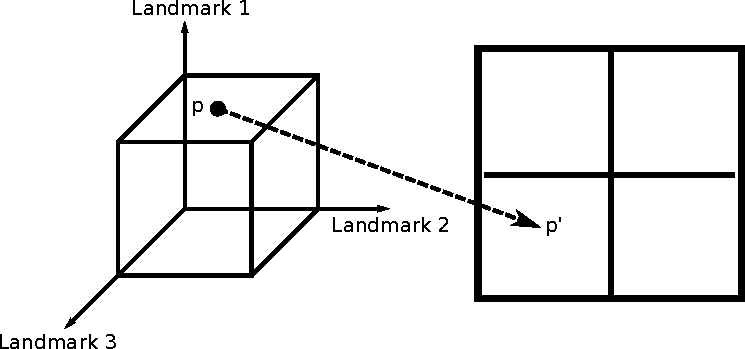
\includegraphics[scale=0.8]{img/algorithms/global_softstate}
\caption{(left) Position of $p$ in the space of $3$ landmarks. (right) Position
of $p$ on the map.}
\label{fig:global_softstate}
\end{figure*}

\textit{Global Soft-State} \cite{xu_globstate_2003} builds a global map to help
choose shorter routing paths, combining the landmark binning method and small
scale distance probes to reveal the proximity properties of the underlying
network to the overlay. Figure \ref{fig:global_softstate} presents the landmark
space and the mapping of the position of the nodes. This global view of the
state is made available to all nodes in order to help them find the best way to
route their messages. \textit{Global Soft-State} operates in two main stages,
generation and use of the proximity information. For generating the proximity
information a hybrid approach is proposed, which uses landmark clustering as a
preprocessing step in order to select a number of potential nearest neighbour
candidates and then refine the selection by incorporating a
round-trip-time-based scheme to ultimately choose the closest node. For using
the proximity information, the algorithm chooses a different path from the
classic gossiping approaches for constructing and maintaining the overlay. It is
based on landmark clustering for strategic placement of proximity information on
the overlay enabling any node to access such information using a landmark number
that reflects its physical position in the network. For various logical
regions\footnote{This might be a high-order zone in the eCAN\cite{xu_ecan_2002}
context or a set of nodes sharing a particular prefix in overlays such as
Pastry.} maps of physical information are built and published where each node
may appear in a maximum of $log\left( N \right)$ such maps. To dynamically adapt
to changing network conditions, a node subscribes to relevant \emph{soft states}
that utilize a notification system in order to initialize any necessary
neighbour re-selection.

Maintaining several host states at different layers, makes any content migration
costly. Additionally, the method does not make any continuing effort to remap
the overlay structure after a node successfully joins, in order to adapt its
  state to any condition change. Although this approach greatly reduces the
  routing latency to far nodes, it is unable to dynamically identify nodes that
  are close to routers and gateways in order to construct the secondary overlay.
Nevertheless, static recognition of such nodes is currently done based on BGP
reports and pre-chosen landmarks, sacrificing the self-organising attribute of
traditional DHTs.

%
% TODO: SOME DISCUSSION
%
% Xu \textit{et al.} \cite{xu_globstate_2003} state that there are three ways
% generating proximity information
%\begin{itemize}
% \item Expanding Ring Search\\
%Expanding ring search can be of two forms. First it can utilize the multicast
%infrastructure in the underlying network in order to emit its messages.
%Unfortunately such infrastructures are not widely deployed thus the
%implementations of this way of generating proximity information is limited to
%blindly flooding the neighbourhood to obtain reasonable results.
%
% \item Heuristics\\
%Heuristics are used in order to reduce the blindness of the expanding ring
%search and make realizations more efficient and effective. Unfortunately a
%common problem of all heuristic approaches is the local minimum pitfall in
%which
%the search might be caught into.
%
% \item Landmark Binning\\
%Landmark clustering is based on the view that nodes with similar distances to a
%set of predefined well-known landmark nodes are pretty likely of being close to
%each other. But this approach has its weaknesses as well, such as the fact that
%is a rather coarse grained approximation, therefore not particularly well
%suited
%for differentiating nodes within close distance to each other.
%
%\end{itemize}
%
%

%
% TODO: IN PAPER INTRODUCTION A DISCUSSION ABOUT
%TOPOLOGY-AWARE CAN
%
%Techniques to exploit topology information in overlay
%routing include geographic layout, proximity routing and
%proximity neighbor selection [3]. With geographic layout
%such as topology-aware CAN [12], the overlay structure is
%constrained by underlying network topology. This tech-
%nique, unfortunately, can create uneven distribution of
%nodes in the overlay, increasing the chances of overloading
%nodes and rendering the maintenance cost formidable. Our
%study shows that, for a typical 10,000-node topology-aware
%CAN, 5% nodes occupy 85-98% of the entire Cartesian
%space, and some nodes have to maintain 450-1500 neigh-
%bors. In Proximity routing, physical topology is not consid-
%ered when constructing the overlay.
%

%%%%%%%%%%%%%%%%%%%%%%%%%%%%%%%%%%%%%%%%%%%%%%%%%%%%%%%%%%%%%%%%%%%%%%%%%%%%%%%%
\subsubsection{Mithos}
\emph{Mithos} \cite{waldvogel_mythos_2003} is a P2P protocol which incorporates
directed incremental probing to find near optimal node placement, and is
classified by its authors as an integration of geographic layout and proximity
routing overlay optimization methods.

The bootstrap phase of Mithos starts with a subset of existing members as the
first set of candidates, and while the iteratively closest nodes are detected by
probing the neighborhood, the candidate neighbor list is updated. In order to
avoid a local minima, Mithos probes all the neighbours within a two-hop distance
from the current minimum before concluding the process.

After finding its first neighbour, the newcomming peer is assigned an ID using
information gathered during the iterative neighbour selection phase. Virtual
coordinates are assigned to the newcomming peer by using the distances of two
closest nodes and their neighbours, so that Euclidean distances between the node
and all known hosts predict the network latency between
them\cite{cox_vivaldi_2004}. The benefit of these synthetic coordinates are that
they are explicitly used as the node's ID, and distance computations among nodes
can be done in ID space without requiring physical measurements.

The last step of the algorithm is the interconnection among neighbours. Mithos
uses a \emph{quadrant-based} mechanism according to which each node establishes
a link to the closest neighbour in each quadrant. During forwarding, the next
hop is performed towards a neighbour in the same quadrant as the final
destination. The newcoming node may not know of other neighbours in all
quadrants, therefore, the node first identifies neighbours in all quadrants
using a mechanism based on ideas similar to a perimeter walk\footnote{Used in
Greedy Perimeter Stateless Routing (GPSR) protocol.} and then improves the
results using parallel path processing by taking into account further geometric
properties of node relationships.

One major limitation of \textit{Mithos} is that the protocol cannot handle
dynamic arrivals and removals from the network, as is happens in mobile
networks.

%
% TODO: review this part
%
%In order to avoid local minima during neighbour detection, extensive probing
%  must be undertaken. In simulation, unfortunately, only very small-sized
% overlay topologies (of 200 to 1000 nodes) have been used and thus no safe
% conclusions can be made as for the behaviour of an extensively large,
% real-world p2p deployment of the scheme.

%%%%%%%%%%%%%%%%%%%%%%%%%%%%%%%%%%%%%%%%%%%%%%%%%%%%%%%%%%%%%%%%%%%%%%%%%%%%%%%%
\subsubsection{LAPTOP}
\emph{LAPTOP} \cite{wu_laptop_2007}, organises the overlay into a tree-based
hierarchy with main focus on reducing hops during message routing as well as
minimizing maintenance overhead. Additionally, a caching scheme is also
incorporated so as to further reduce routing table update costs. The authors
theoretically show that in LAPTOP routing path length is bounded by $O(log_d N)$
and node joining and leaving in the overlay network is bounded by
$O\left( d log_d N \right)$ hops in a balanced overlay tree, where $N$ is the
number of nodes, and $d$ is the maximum degree of each node. LAPTOP implements
the geographical layout approach  and constructs its layout in a self-organizing
and efficient fashion, by estimating the round-trip times to a small number of
nodes in the overlay network in order to make them roughly aware of their
physical distances among them.

Each node is assigned a dot-formated address (e.g 1.3.4). Each octet ranges from
$1$ to $d$, where $d$ is the maximum degree of the nodes. The assignment process
is done by appending a unique octet to the address of each nodes parent, while
root node is assigned address $1$.

%The protocol is based on four definitions.
%\begin{enumerate}
% \item The amplitude of all possible measured RTTs is devided into intervals.
%  Each node measures its distance to its parent and is assigned a label $L_i$
% where $i$ denotes the configurable RTT interval in which the measured distance
% falls into. A special kind of node, the root, is initially assigned the $L_1$
% label and maintains (as all $L_1$ nodes do) a list of other $L_1$ nodes in the
% overlay.
% \item Any node can have children with level lower than theirs, except an
%  $L_{max}$ node which can only have $L_{max}$ level children and only in the
% case when its parent has reached its maximum degree.
% \item Each node is assigned a dot-formated address (e.g 1.3.4). Each octet
% ranges from
% $1$ to $d$, where $d$ is the maximum degree of the nodes. The assignment
% process
% is done by appending a unique octet to the address of each nodes parent, while
% root node is assigned address $1$.
% \item For any descendant node $Y$ of a node $X$, the measured distance among
%  each other, must always be less than the lower bound of the RTT interval
% denoted by $X$'s label.
%\end{enumerate}
%

The routing scheme is similar to the longest-prefix IP matching scheme. At each
forwarding hop, any message travels up the tree until the first common ancestor
of both source and destination nodes is reached and then starts descending to
arrive to its target. During tree traversals, special entries in the routing
tables, called \emph{routing cache}, are maintained in order to increase routing
efficiency and achieve finer load balance. Caching enables a node to forward a
message to a better longest-prefix match than that of its direct ancestor making
a larger, quicker and more cost effective step through the overlay and toward
the destination. To improve scalability, the number of children nodes and the
size of the routing cache are limited. In terms of overlay maintenance, LAPTOP
incorporates a simple \emph{heartbeat}-based technique where each parent node is
responsible for monitoring its children.

%
%The newcommer $N$ locates the root node and the later responds with a list of
%  $L_1$ nodes. $N$ then probes each of the $L_1$ nodes in search for the
% closest one. If the measured RTT to the closest $L_1$ falls into the first
% interval then the newcommer becomes a $L_1$ node as well. Otherwise node $N$
% sets the closest $L_1$ node as its potential parent node. This potential
% parent becomes the actual parent if it does not have any other children. If it
% has, $N$ gets a list of these $L_i$ nodes and by measuring the RTT to each of
% them tries to spot a new potential parent in order to repeat the above
% process.
%

% At join process the newcomming node is assigned its level label as well as its
% address by its parent node. Additionally, it initializes its routing table
%(with normal and caching entries) as it traverses the overlay in search for
%its parent node.  During a graceful departure, the referred node checks for
%children in the overlay. If it does not have any, it simply notifies its
%parent and leaves. If it has, it selects the child node with the lowest
%round-trip time to it in order to take its place so that the locality
%property is preserved. On the other hand, in the case of an arbitrary
%failure, after the children of the failed node detect their parent's absence
%(throught the aformentioned heartbeat mechanism), they start emmiting special
%messages to their grandparent node (the address of which is stored during
%join process}. In case of no response from the grandparent node, the children
%invoke the joining process to detect their new parent node.The parent of the
%failed node, aggregates the notifications from the above children nodes for a
%period of time, and then chooses the one with the lowest level label as the
%takeover node. Potential ties are broken by favouring the lower RTT. The
%parent of the failed node, finally informs accordingly all the children about
%the change in the hierarchy.

%%%%%%%%%%%%%%%%%%%%%%%%%%%%%%%%%%%%%%%%%%%%%%%%%%%%%%%%%%%%%%%%%%%%%%%%%%%%%%%%
%
% TODO: HERE STRUCTURED LANDMARK BINING APPROCH LIES
%
%Assuming a structured approach based on CAN\cite{ratnasamy_can_2001} and $m$
% landmark nodes. The coordinate space is then partitioned into $m!$ equally
%sized portions, each corresonding to a single ordering of the landmarks. To do
%this, the first dimension is divided into $m$ areas each of which is furtherly
%divided (second dimension) into $m - 1$ sections and so on. Having set this $m$
%dimensional space, at joining time, a node measures the delay to the set of
%landmarks in order to determine its associated bin and thus position itself in
%that portion of the coordinate space associated with its landmark ordering.
%Even though this scheme can
%



%###############################################################################
%###############################################################################
%###############################################################################
%       PROXIMITY ROUTING
%###############################################################################
%###############################################################################
%###############################################################################


%%%%%%%%%%%%%%%%%%%%%%%%%%%%%%%%%%%%%%%%%%%%%%%%%%%%%%%%%%%%%%%%%%%%%%%%%%%%%%%%
\subsubsection{Proximity in Kademlia}
% Before discussing {\em Proximity in Kademlia}, it would be helpful to briefly
% summarize the highlights about the {\em Kademlia} protocol. {\em Kademlia}
% \cite{maymounkov_kademlia_2002} is a distributed hash table (DHT) based
% protocol for P2P networks, which uses an iteration based lookup algorithm. The
% protocol uses the standard $160$ bit ID system for nodes and locates the nodes
% in a prefix binary tree, where IDs are used as prefixes. The iterative lookup
% operations are done over this prefix binary tree, which converges to
%logarithmic
% lookup times. The ID's are assigned randomly, therefore in Kademlia, there is
%no
% proximity control, which results in inefficient use of the underlying network
% during lookup and retrieve operations.

\emph{Proximity in Kademlia} \cite{kaune_pkad_2008} introduces proximity
controls over the vanilla Kademlia protocol's random ID assignment, in order to
optimize the underlying network usage of the protocol. The work in this paper
can also be considered, as a more generic study over building proximity in the
context of iterative lookup algorithms. Focus is given on both the overlay and
the underlaying tiers in the sense that in the first improves the routing
performance according to a cost metric that is provided by the later and
quantifies the suitability of establishing a communication link between peers as
a cost function, based on the used proximity criteria (RTT, ISP locality, etc.).
%An underlay metric provides information about the underlay network. The paper
%  distingushes between three kinds of possibilities to quantify it:
%\begin{itemize}
% \item Using measurements gained by previous lookups
% \item Using measurements acquired by other peers or jointly calculated with
%  others
% \item Using a local database to look up information
%\end{itemize}
The paper proposes two approaches for overlay optimisation. One falling into
{\em proximity routing} and the other on {\em proximity neighbour selection}
approaches overlay optimization techiques for
exploiting proximity. For the first, the goal is in choosing the best next hop
during routing a message. Due to the fact that the routing in Kademlia is
iterative, it is the initiator of the lookup that chooses each next hop from a
set of candidate nodes. Standard Kedemlia always chooses the closest node with
respect to the XOR metric but with proximity routing selection, Kademlia
chooses the one with the smallest underlay metric cost. Thus, as in all such
approaches, there is a trade-off between the overlay and underlay distances.

Toward the enhancement of traffic locality, the authors also use information
from the MaxMind GeoIP database\footnote{MaxMind Geolocation Technology.
http://www.maxmind.com} to retrieve proximity information of a given
peer based on its region, country, or ISP location, and use this information to
form clusters of nearby peers. An alternative method could also be the use of 
Vivaldi coordinates \cite{cox_vivaldi_2004}. However, authors report that
clustering approach performs better than Vivaldi protocol based on their
experiments. Authors also report that {\em Proximity routing} protocol
successfully worked with the Kademlia protocol and improved the locality of the
connections over peers.

As already mentioned the paper
proposes \emph{proximity neighbour selection} method, as well, for overlay
optimisation. The goal, according to this, is to keep peers with the least
contact cost in the routing table. As Kademlia constantly learns new peers
(incoming requests, through iterative lookup) no special algorithm for
searching more cost effective peers is necessary and simply choose the best
peers seen so far.

%%%%%%%%%%%%%%%%%%%%%%%%%%%%%%%%%%%%%%%%%%%%%%%%%%%%%%%%%%%%%%%%%%%%%%%%%%%%%%%%
\subsubsection{CHOord considering Proximity on IPv6 (CHOP6)}
\emph{CHOP6} \cite{morimoto_chop6_2007} roughly estimates the proximity among
nodes by exploiting the IPv6 address format and RTT information if available.
The proximity estimation is achieved by introducing a 64-bit ID scheme in which
the least significant bit part is the IPv6 global routing prefix and thus
enabling a longest prefix match scheme. The protocol is designed based on the
observation that it is possible to estimate a node's geographical location by
simply examining the upper 32-bits of its IPv6 address. Moreover, similar to
Chord, CHOP6 uses a finger table, whose entries hold more than
one candidate node.

%
%\paragraph{}
% There are three cases in which a node chooses the next hop according to
% information it posseses.
%\begin{itemize}
% \item When no information about RTT is available candidate next hops, the
%  sender just selects a node in the finger table entry which shares the longest
% prefix with the destination.
% \item There is another possibility that after some communication with other
%  nodes, the source node should know of the RTTs to some of the nodes in finger
% table entry. In this case, the source node chooses the one with the smallest
% RTT with propability $p$. If there is a node with no measured RTT then the
% sender can select such a node with probability $1 - p$
% \item In this last case the source node has already communicated with all
%  candidate node in the finger table entry. Thus, the node selects the node
% whose RTT is the smallest with probability $p$, the one with the second
% smallest with probability $q$ and so on, where $0 \leq \ldots < r < q < p < 1$
% and $p+q+r+\ldots \leq 1$
%\end{itemize}
%

%%%%%%%%%%%%%%%%%%%%%%%%%%%%%%%%%%%%%%%%%%%%%%%%%%%%%%%%%%%%%%%%%%%%%%%%%%%%%%%%
\subsubsection{T2MC}
T2MC \cite{shi_t2mc_2008} uses traceroute logs to detect different autonomous
systems and cluster close by peers, thus reducing redundant traffic that crosses
autonomous system boundaries. T2MC uses a customized k-mean classification
algorithm with $k=2$ to perform the classification, and exploits the stable
structure of the Internet routers to guide clustering. The peer chooses the
minimum and maximum Latency results from the traceroute to initialize the
centroinds of two sets. Then the peer calculates, for all hops allong its
tracerouted path, the absolute distance to these centroids of both sets and
assigns the routers to that centroid with which it has the smaller absolute
distance. After that, the mean and variance values are calculated and if the
variance is larger than a predefined threshold then the algorithm sets the two
latency mean values as new centroids for the two sets and loops again.
Ultimately peer will end up with two sets having the minimum intra-set variance.
The peer, then, chooses the router from the second set with the minimum hops
attribute and sets it as a threshold. The selected router and all others whose
hops attribute is larger than the threshold are classified as \emph{remote}
router cluster. The remaining are classified as \emph{near}. From the near
class, the peer chooses the one with maximum hops attribute as its edge router,
and registers it along with the all the near cluster into the DHT of the P2P
overlay. As new peers join the network, those that share the same edge router
or any of the members of the near router clustersm there would gather to form a
close peer cluster. As Edge routers can provide more valuable information than
other members of the near set, T2MC was designed to prioritize interaction of
peers and edge gateways.

%
% TODO: SOME DISCUSSION
%
%The use of Traceroute as a tool for implementing the distance measuring
%infrastructure raise concearns about its efficiency and scalability. Being,
%primarilly, a network diagnostic utility, it is concearned too heavy weighted
%and intrucive for use in a larger scale\cite{ratnasamy_binning_2002}.
%Additionally, disabling ICMP is a common administrative policy for edge sites
%to enforce security, while dumping BGP routing
%tables\cite{krishnamurthy_bgpclust_2000} is not directly available to the
%application layer.
% Even though traceroute provides detailed information about the network
% structure, its excessive use creates additional overhead that stresses further
% the overall network infrastructure. This forces network administrators to
% disable its support from the routers they manage, thus jeopardizing the
% effectiveness of the T2MC algorithm.
%

%%%%%%%%%%%%%%%%%%%%%%%%%%%%%%%%%%%%%%%%%%%%%%%%%%%%%%%%%%%%%%%%%%%%%%%%%%%%%%%%
\subsubsection{PChord}
\emph{PChord}\cite{hong_pchord_2005} is a based on the Chord DHT which adds
proximity routing into its routing mechanism. The main modification over the
vanilla Chord is the inclusion of a \emph{proximity list} into its routing table
so that the next hop is decided based not only by considering best progress
towards the key, but on the physical proximity of the candidate nodes as well.
The list is, at join time, empty but as the PChord node starts to interact with
other nodes it applies a heuristic mechanism to fill up the list. Entries are
dynamicaly added or removed as the network state changes. Due to the fact that,
with each step, there is always progress towards the target node in the ID
space, PChord will result in a reduced hop number than Chord, since each hop in
PChord is larger or at least equal in the key space. Passing through proximity
links in the underlaying network means reduced routing cost. Additionally, if
the number of entries in the proximity list is the same as the number of network
partitions, PChord prevents hops from jumping in and out the network partition
the current node belongs to.

%%%%%%%%%%%%%%%%%%%%%%%%%%%%%%%%%%%%%%%%%%%%%%%%%%%%%%%%%%%%%%%%%%%%%%%%%%%%%%%%
\subsubsection{AChord}
\emph{AChord} \cite{dao_achord_2006} uses IPv6's anycast mechanism in order to
releave the protocol from complex joining procedures, and achieve high accuracy
of network proximity giving high routing efficiency, Anycast delivers a message
comming from the outside of an anycast group to the physicaly closest node in
that group. AChord organizes all nodes participating in the overlay network into
an anycast group. Any joining node comes outside of that group and, thus, is
automaticaly forwarded to the physicaly nearest node in order to bootstrap,
avoiding the need to, explicitly, maintain such nodes, and the effort of finding
a way of locating the physically nearest among them. The ID of the new comming
node is computed based on the ID of the bootstrap node and the bootstrap's
predecessor in a way that the constructed ID will be positioned between the
aformentioned two. After joining, the finger table is build the same way as in
the Chord protocol. Moreover, additional nodes are maintained in a structure
called \emph{neighbourship table} which stores information about the closest
known node. The routing decision is made by using both the neighbourship and
the finger table. The authors claim this to be a lightweight approach that
requires few changes to Chord in order not to affecting its own advantageous
characteristics.

%%%%%%%%%%%%%%%%%%%%%%%%%%%%%%%%%%%%%%%%%%%%%%%%%%%%%%%%%%%%%%%%%%%%%%%%%%%%%%%%
\subsubsection{Chord6}
\emph{Chord6} \cite{xiong_chord6_2005} is another Chord variant that tries to
exploit the hierarchical features of IPv6 in order to create a substrate that
reduces interdomain traffic between service providers. The difference between
Chord6 and Chord the identifier definition. Therefore, the approach can be
easily portable to other DHTs such as CAN, Pastry and Tapestry. In Chord6 the
identifier contains two parts: the higher bits are obtained by hashing the
node's IPv6 address prefix of specific length, while the remaining lower bits
are the hash value of the rest of that IPv6 address. As a result of this
assignment, nodes in a domain will be mapped onto a continuous key space on the
overlay network, which avoids unnecessary message forwarding across different
service providers, thus minimising overall routing cost.

%
% TODO: SOME DISCUSSION
% However, even though nodes in the same domain would have close identifiers,
% nodes in two close domains may have very different ones.




%###############################################################################
%###############################################################################
%###############################################################################
%       PROXIMITY NEIGHBOUR SELECTION
%###############################################################################
%###############################################################################
%###############################################################################

%%%%%%%%%%%%%%%%%%%%%%%%%%%%%%%%%%%%%%%%%%%%%%%%%%%%%%%%%%%%%%%%%%%%%%%%%%%%%%%%
\subsubsection{DHT-PNS}
The work in \cite{hancong_pnsbased_2006} propose a proximity neighbour selection
scheme on top of the Chord DHT. The main goal is to use proximity information
to group physically close by nodes as neighbours in the DHT table. In order to
detect proximity, virtual network coordinates of peers are used, by using the
Vivaldi protocol \cite{cox_vivaldi_2004}. The virtual coordinates are then used
by the nodes to map to identifier space in the DHT. The space is partitioned
using a \emph{concentric circle clustering scheme} where successive cycles of
radiuses $\rho$, $2\rho$, $3\rho$ and so on, are constructed. Then the formed
annuluses are divided into $2\chi-1$ \emph{sectors}, where $\chi$ denotes the
sequence number of the annulus starting from $\chi = 1$ for the centre cycle. It
is proved in the paper, that this way each sector occupies the same area as does
the center cycle. Assuming uniform node distribution, this characteristic,
favours a more load balanced clustering operation. Every sector in this $2d$
coordinate space is mapped to a unique \emph{region} in the DHT space forming a
multi-layer node identifier space.  Thus, any nodes that belong to the same
sector, are mapped to the same region as well, preserving their proximity
relationship unveiled by the use of the Vivaldi protocol. The individual pieces
are mapped to the identifier space uniquely, allowing logarithmic lookup
operations with high probability on Chord. The system described in the previous
section allows any node to obtain its DHT key and its region key, in a fully
distributed manner, just by applying a consistent hash function. Using an RPC
call in Chord, the node can obtain the region's master node, called
\emph{Cluster Node (CN)} which is responsible for clustering the nodes belonging
in the same sector or region with that of the node at hand. An additional RPC
call, registers it to its corresponding region and publishes its information,
through the special peer CN. The node can, additionaly, ask CN for other
nodes that have previously joined the region in order to add them into its
neighbour set for future routing table optimization. Even in the case when no
neighbour is detected in the current region, the search is expanded to adjasent
regions and towards an upper layer identifier space until one is found or the
first layer reached.

%%%%%%%%%%%%%%%%%%%%%%%%%%%%%%%%%%%%%%%%%%%%%%%%%%%%%%%%%%%%%%%%%%%%%%%%%%%%%%%%
\subsubsection{Quasi-Chord}
The approach that is proposed by Sun and Zhang in \cite{sun_quasi_2008}
confronts the topology mismatch problem, in the Chord DHT context which, in its
vanilla version, takes no consiteration for the underlying physical network
topology during the construction of the identifier cycle. To construct a
\emph{Quasi-Chord} network three steps are followed needed. First, each host
acquires its coordinates in the geometric space utilizing the \emph{global
network position (GNP)} protocol \cite{ng_gnp_2001}. Second, using the
\emph{Cantor space filling curve}, the $2$-dimensional space is converted to a
$1$-dimensional one, used in the last, third, step to build the Quasi-Chord
circle according to the host's Cantor value.


%In the following paragraphs, these steps are furtherly discussed.
%
%\paragraph{GNP coordinates}
%First of all the host must be positioned in the geometric space. The algoritm
%  models the P2P network with a well defined distance function in such a way,
% it can predict, with high accuracy, the distance between any two points in the
% space by just evaluating the output of the distance function on the
% coordinates of these points. This is accomplished with the \emph{global
% network position (GNP)} protocol which\begin{inparaenum}[\itshape i\upshape)]
%  \item creates a reference set of $N$ landmark nodes so as to minimize the
%  error of ICMP measured distances and coordinate computed ones between them,
% and then
%  \item each host is able to measure its round-trip times to the $N$ Landmarks
% in order to compute its own coordinates.
%\end{inparaenum}
%
%\paragraph{Cantor SPF}
%After the $2$-d coordinates are set, in the next stage of the algorithn, each
%  participating peer is assigned a Cantor value, according to the application
% of a \emph{space filling curve} on the coordinate space. (TODO: add figure).
% This results in the conversion of the $2$-dimensional space to a
% $1$-dimensional Cantor space that can more easily be more mapped to the Chord
% hierarchy.
%
%\paragraph{Quasi-Chord construction}
%As can intuitively be infered by observing the Cantor chart, close-by nodes in
%  the physical layer, are more likely to have similar Cantor values. This
% attribute is exploited in order to construct a topology-aware identifier space
% for the Chord DHT. The cycle is constructed by sorting nodes in ascending
% order. Each host maintains 2 finger tables, one for clockwise and one for
% counter-clockwise stepping. This helps with the connectivity of the network
% because its not allowed to connect the first node with the last one since this
% will incur heavy traffic to the later\footnote{After all their Cantor values
% denote that they are actually the furthest of each other.}.
%

%
% TODO: SOME DISCUSSION
%       NEEDS DOUBLECHECK
%
%The disadvantage of the algorithm is that the coordinate assignment in the
%  first stage is backed by a not fully distributed landmark-based algorithm.
% Moreover the Quasi-Chord model build-up is making an indirect assumption of a
% maximum number of allowable hosts since it is constructed. Last but not least
% the doubling of the required routing information which needs to be created and
% maintained is an additional negative point to the efficiency and the
% scallability of the algorithm.
%

%%%%%%%%%%%%%%%%%%%%%%%%%%%%%%%%%%%%%%%%%%%%%%%%%%%%%%%%%%%%%%%%%%%%%%%%%%%%%%%%
\subsubsection{IP-based Clustering (IPBC)}
Proximity neighbour selection algorithms use probing and other techniques to
detect proximity. However, such methods are either not precise enough, or
overload the network. \emph{IP-based clustering} \cite{karwaczynski_ipbc_2007}
is a proximity neighbour selection based algorithm in which the authors propose
to use the IP address prefixes (16 bit for IPv4) in order to detect proximity.
\cite{freedman_iploc_2005} states that $97\%$ of prefixes larger than $24$ bits
belong to a single geographical location. However, using less number of bits
creates less precise results and more number of bits increase the burden on the
network and reduce the possible number of neighbours. Therefore, a careful
selection is required in terms of performance/accuracy tradeoff. IP-based
Clustering generates a key and its prefix and stores the later in the DHT
itself, so that any newly joining nodes with the same IP prefix can query it and
identify all the neighbours with the same one relatively easy. Nodes
periodically update their entries in the DHT by removing those who leave, or
those who has been timed out with no further activity detected from the node.

% Moreover, observing the
% \emph{IANA IPv4 Address Space Registry} we can infer that, since blocks of
% consecutive octet prefixes are assigned to the same Regional Internet
% Registries (RIRs), nodes inside will be physicaly close to each other.

%
% In order to be published in the overlay, each node is first assigned a
% unique identifier and subsequently generates a key by hashing a fixed-length
% prefix of its IP. Authors argue on the prefix length to be used, as there is a
% thin balance between reducing the propability of finding closer nodes by
% adopting a long prefix and overload nodes that are responsible for information
% published by many peers when chosing to hash a short one. Their verdict is for
% the use of a 16-bit wide prefix for real world systems deployed in an Internet
% scale. In either case, ID and IP is then stored in the DHT using this
% generated key. This way, any node, at any time (either at join time or during
% peer lifetime for topology adaptation) can acquire information about close-by
% nodes just by quering thde DHT for a specific key. Moreover, the algorithm
% takes care of the freshness of the proximity information in two ways. First,
% the advertising nodes themselves periodically update their advertisements or
% when they voluntarily leave the overlay, they explicitly remove their data. On
% the other hand, in case of a failure each publication is assigned an
% expiration time, and thus ultimately removed by the DHT maintenance
%mechanisms.
%

%%%%%%%%%%%%%%%%%%%%%%%%%%%%%%%%%%%%%%%%%%%%%%%%%%%%%%%%%%%%%%%%%%%%%%%%%%%%%%%%
\subsubsection{Cone}
\emph{Cone} \cite{wang_cone_2007} extends Chord using proximity neighbour
selection topology optimization algorithm. The proximity information is
generated using landmarks and round-trip-time-based distances to landmarks.
Cone uses a two-layered identifier space. The first, named Chord-layer
identifier, denoted as $Id_{Chord}$, is the same as in Chord. The second is the
Cone-layer identifier, $Id_{Cone}$ which is constructed by two component
identifiers. The first, known as \emph{group identifier (gid)} denotes a
relevant group the node belongs to while the second, namely \emph{local
identifier (lid)} indicates the local identifier within the group. The group
concept, which is introduced here, is a way of dividing nodes according to a
common $Id_{Chord}$ prefix.  The structure of a Cone overlay, retains the
Chord's circular topology. The difference lies on the fact that, now, two rings
are created. A big ring, where nodes with the same \emph{gid} are arranged at
each position. Each of these positions are a smaller ring for the particular
group's \emph{lid}s. The routing is achieved in both clockwise and
counter-clockwise directions in the big-ring, for which two routing tables are
maintained, namely \emph{front} and \emph{back} finger tables. Entries in these
tables, display physical network proximity with the current node. Moreover, a
third table called \emph{group} maintains information about other online peers
within the current node's group in a way that entries are now close in the ID
space.

%
%Routing in Cone, comprises of the inter-group algoritm and the intra-group
%  algorithm. First the group of nodes to which the desired key lies is
% detected, exploiting physical proximity information (front and back finger
% tables). Second during the next and last hop, the message is forwarded to the
% exact node that contains the desired key.
%

%%%%%%%%%%%%%%%%%%%%%%%%%%%%%%%%%%%%%%%%%%%%%%%%%%%%%%%%%%%%%%%%%%%%%%%%%%%%%%%%
\subsubsection{DynaMo}
\emph{DynaMO} \cite{winter_dynamo_2004} tries to build an overlay that not only 
considers physical proximity among peers but their mobility attributes as well.
DynaMO is based on a Pastry overlay network and this was a preety concious
choice, by the authors, basically because of Pastry's built-in locality
heuristics which are thoroughly analysed in the in the literature
\cite{castro_proximityp2p_2002} providing good backround against which to test
and compare their results. In order to adapt to mobile, ad-hoc networks,
though, special care has been put to the maintenance of an even overlay ID
distribution so that hot-spots are avoided. DynaMO dictates a newcoming node to
gather information concerning its physical neighbourhood and uses it to assign
itself an appropriate overlay ID. DynaMO tries to capitalize on the fact that
in Pastry each node's table consists of rows equal to the number of digits of
the overlay IDs and columns equal to the ID's base. As we go down the table
rows, the matching prefix between the current node's ID and the row's entries
increases by one. Thus, the leaf set contains the closest nodes in the ID space.
Additionally as the prefix match increases by one, the result is exponentially
less candidates that can fill the tables entries as the row increases. This
leads to the observation \cite{antony_pastry_2001,castro_proximityp2p_2002} that
from overlay routing hop to overlay routing hop the physical distance between
nodes is likely to increase leading to a dominating last routing step in terms
of the overall plysical routing path distance travelled during a key lookup.
Since the last routing step is usually taken from the leaf set, DynaMO focuses
on making this last step as physicaly close as possible. In this context, two
approaches are considered namely \emph{Random Landmarking (RLM)} and
\emph{Closest Neighbour Prefix Assignment (CNPA)}.

RLM lookup mechanism to locate nodes responsible for a fixed set of carefully
chosen (in a way that the ID space is divided into equal portions) landmark
keys. This means that when a node is assigned a landmark key then it plays the
role of a temporary landmark for the network. Any joing node will measure its
distance to that and all other landmarks and assign to itself an ID consisting
of a prefix taken from the closest landmark and a remainder that could be
assigned randomnly or generated by mechanism that takes into account physical
neighbourhood. The legth of the prefix can be determined as
$prefix_length=|log_b k|$, where $b$ is the ID base and $k$ the number of
landmarks. The above scheme results in physically close nodes, forming regions
of common ID prefix that are likely to be close to each other in the ID space
and thus bringing a node's leaf set closer to itself. Additionally, the
advantage of dynamic landmark nodes is that the failed ones can instantly be
replaced by new responsibles, that share similar physical attributes to the
failed and thus preserving the balance of the network.

RLM may incur more traffic especially on landmark nodes, load that in some cases
is not acceptable. CPNA on the other hand takes advantage of Pastry's
specification that a new coming node is bootstraped by a physicaly close node.
The new comer then assumes the ID prefix of that neighbour while the rest is
generated similarly to RLM. Unfortunately, less overhead comes at the expense
of being more coarse-grained.

%
% TODO: SOME DISCUSSION
%
%Both algorithms, are protected against the formation of physical landmark
%  clusters or imbalanced ID distribution\footnote{More common during the
% initial formation of an overlay network} , by introducing the \emph{landmark
% gravitation range} as a theshold over which landmark keys are reassinged (for
% the RLM approach) or unutilized ID prefix ranges are detected and used (for
% the CPNA scheme) in order to balance the distribution of regions in the
% overlay.
%

%%%%%%%%%%%%%%%%%%%%%%%%%%%%%%%%%%%%%%%%%%%%%%%%%%%%%%%%%%%%%%%%%%%%%%%%%%%%%%%%
\subsubsection{SAT-Match: Self-Adaptive Topology Matching}

\begin{figure}[ht]
\centering
\subfigure[Example physical topology of nodes.] {
  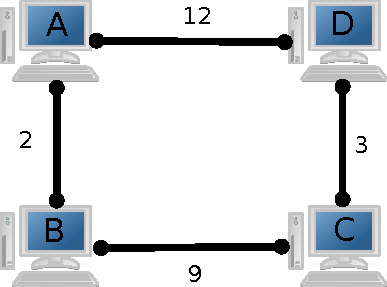
\includegraphics[scale=0.6]{img/algorithms/SAT_match}
  \label{figure:sat_match:before}
}\qquad\qquad
\subfigure[(left) A jumps to B in order to match the logical topology to the
physical. (right) State of the logical topology after the jump.] {
  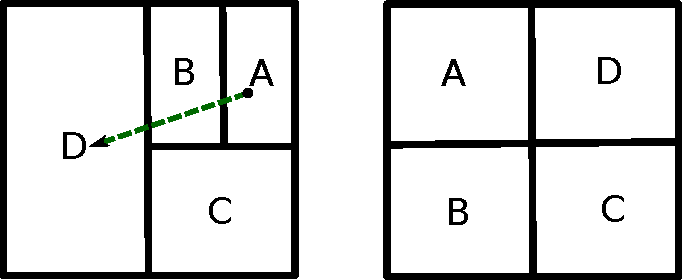
\includegraphics[scale=0.6]{img/algorithms/SAT_match2}
  \label{figure:sat_match:after}
}
\caption{The SAT-Match algorithm.}
\label{figure:sat_match}
\end{figure}

\emph{SAT-Match} \cite{ren_satmatch_2004}. Even though no theoretical proof is
given, valid results are obtained and demonstrated through experimentations.
Similar to the other approaches in the proximity neighbour selection,
\textit{SAT-Match} uses probing to detect close by peers and obtain proximity
information. However, as an additional feature, SAT-Match peers can do
selective jumps to adjust their positioning in the DHT, if it reduces the
\emph{stretch} of its one-hop neighbourhood. The paper defines stretch
$S = \frac{\bar{L_l}}{\bar{L_p}}$, where $\bar{L_l}$ is the average
logical link latency while the $\bar{L_p}$ is the average physical
link latency, and uses it a way quantify the \emph{topology
match degree} of the constructed overlay. For the probing phase SAT-Match uses a
small TTL value for the probing messages in order to reduce
redundancy\cite{jiang_lightflood_2008}. This process begins as soon as the node
joins the network using a DHT mechanism. Each probing message contains
information about the source and a small TTL value. The recipient of such a
message returns information about itself to the source and forwards the probing
message to its neighbours if the TTL is non-zero. The discovered nodes are
referred to as $TTL-k$ neighbourhood of the source node based on the $TTL$
distance to the source node. Blindly selecting the peer with the smallest RTT
as neighbour is, generally, not the optimal decision to make in order to achieve
global stretch reduction. In a structured scheme, when a node jumps to connect
to a physically close node, it may need to connect to other distant nodes to
maintain the structure's integrity, thus creating an overall increase in the
overlay's stretch. The two nodes with the smallest RTT are then used in order to
select one zone to jump in this phase. The algorithm is as follows: The source
node $S$ calculates the stretch change of its $TTL-1$ neighbourhood and that of
the $TTL-1$ neighbourhood of the first of the previously selected peers. These
calculations are made as if the jump has been made. If the stretch reduction is
over a predefined threshold the jump is performed, otherwise the second selected
candidate is picked and the same computations are performed. If again, the
threshold is not met, then no jump is ultimately done. In case of a jump, this
is performed as a combination of \emph{leave} and \emph{join} operations, in the
CAN context. Figure~\ref{figure:sat_match} demonstrates the selective jump on an
example topology.

%
%\paragraph{}
%Moreover the algorithm takes several issues into consiteration in order to
%  furtherly improve the resulted overlay. For example when multiple nodes try
% to jump simultaneously into a region, then the logical link brakes from one
% attempt may result in inacurate computation of the gain factor, for an other.
% This situation is identified as \emph{contention} and the nodes use an
% exponatial back-off algorithm to avoid it. An other problem is the uneseccary
% traffic incuerred by the probing phase in a region that after several jumps
% has settled to a stable state. In these cases it is more likely for jump
% attempts to be proven worthless. The algorithm doubles the probing period of
% such nodes, every time a jump is not taken.
%
%\paragraph{}
%The authors claim that this continuously adaptive mechanism achieves global
%  topology matching optimization in a sufficiently large scope. This also
% secures the fast adaptation to frequent network changes. It also considered
% lightweight and can easily be embedded into current p2p systems, as well
% as effectively combined with other techniques, such as landmark binning.

%
% TODO: SOME DISCUSSION
%
% It is reported that,
% due to the selective jumps, SAT-Match achieves $40\%$ reduction in
% link stretch, and when used with the landmark binning (see
% Sec. \ref{sec:landmark_binning}), the reduction rate increases up to $60\%$.
% For dynamic environments, with frequent node arrival and leave, SAT-Match
% scales much better than Mithos, due to its self adaptation mechanism and
% selective jumps.

%%%%%%%%%%%%%%%%%%%%%%%%%%%%%%%%%%%%%%%%%%%%%%%%%%%%%%%%%%%%%%%%%%%%%%%%%%%%%%%%
\paragraph*{ \bf Delay Aware P2P System}
A new \emph{Delay Aware P2P System (DAPS)} is introduced in
\cite{zhang_daps_2005}. Its main goal is to reduce the time $L$ of a look-up
request by dividing the routing tables of peers into several sectors in
increasing delay. The source node emitting the query message defines a delay
boundary or the pruning factor $L_t$ in the paper's context. Request messages
will be forwarded only to nodes whose delay less than or equal to $L_t$. With
the clustered routing tables and the loose organisation the overlay network of
\emph{DAPS} is between structured and unstructured.







%%%%%%%%%%%%%%%%%%%%%%%%%%%%%%%%%%%%%%%%%%%%%%%%%%%%%%%%%%%%%%%%%%%%%%%%%%%%%%%%
%%%%%%%%%%%%%%%%%%%%%%%%%%%%%%%%%%%%%%%%%%%%%%%%%%%%%%%%%%%%%%%%%%%%%%%%%%%%%%%%
\subsection{Discussion on the Algorithms for Structured Architectures}
%%%%%%%%%%%%%%%%%%%%%%%%%%%%%%%%%%%%%%%%%%%%%%%%%%%%%%%%%%%%%%%%%%%%%%%%%%%%%%%%
%%%%%%%%%%%%%%%%%%%%%%%%%%%%%%%%%%%%%%%%%%%%%%%%%%%%%%%%%%%%%%%%%%%%%%%%%%%%%%%%



%\begin{figure}[h!]
\hspace{-3ex}
\begin{center}
\footnotesize
%\begin{landscape}
\begin{longtable}{
|>{\columncolor[gray]{.7}}m{0.2\columnwidth}
|>{\columncolor[gray]{.9}}m{0.4\columnwidth}
|>{\columncolor[gray]{.8}}m{0.2\columnwidth}
|>{\columncolor[gray]{.9}}m{0.2\columnwidth}
%|>{\columncolor[gray]{.9}}m{0.1\columnwidth}
%|>{\columncolor[gray]{.8}}m{0.1\columnwidth}
%|>{\columncolor[gray]{.9}}m{0.1\columnwidth}
%|>{\columncolor[gray]{.8}}m{0.1\columnwidth}
|}
\caption{Decentralized Structured Algorithms}\label{fig:struct_compare_table}\\
\hline
\rowcolor[gray]{.5}
\textbf{Algorithm} & \textbf{Overlay structure} & \textbf{Base protocol} & \textbf{Scalability} \\
\hline
\endfirsthead
\multicolumn{4}{c}%
{\tablename\ \thetable\ -- \textit{Continued from previous page}} \\
\hline
\rowcolor[gray]{.5}
\textbf{Algorithm} & \textbf{Overlay structure} & \textbf{Base protocol} & \textbf{Scalability} \\
\hline
\endhead
\hline \multicolumn{4}{r}{\textit{Continued on next page}} \\
\endfoot
\hline
\endlastfoot

\hline
\textbf{Global Softstate} &
\textbf{Geographic layout} Uses first landmark clustering
then measures RTTs to identify close nodes &  &  \\

\hline
\textbf{Mithos} &
\textbf{Geographic layout} Uses nodes as topology landmarks and directed
incremental probing to optimize topology & & Scales well as all
operations are local ??? \\

\hline
\textbf{Self-Adaptive Topology Matching} &
\textbf{Proximity neighbour selection} Uses lightweight probing and
selective jumps to optimize the topology & CAN &  Better than Mithos \\

\hline
\textbf{Delay Aware P2P System} & \textbf{} & & \\

\hline
\textbf{VERSION OF CHORD - DHT-PNS} &
\textbf{Proximity neighbour selection} Uses Proximity Neighbour Selection and the Vivaldi
system & Chord  &  \\

\hline
\textbf{MAY OMIT- VERSION OF CHORD - Quasi-Chord} &
\textbf{Proximity based}  & Chord  &  \\

\hline
\textbf{LAPTOP} &
\textbf{Geographic layout} Hierarchical overlay structure  &  & routing path length $\log{_d N}$,
join/leave overhead $d\log{_d N}$ \\

\hline
\textbf{IP-Based Clustering} &
\textbf{Proximity neighbour selection} Proximity neighbour selection based on longest common
prefix of IP addresses &    &  \\

\hline
\textbf{CHOord considering Proximity on IPv6} &
\textbf{Proximity routing} Uses IPv6 address format to provide proximity &  Chord
 & Better than Chord \\

\hline
\textbf{Proximity in Kademlia} &
\textbf{Proximity routing} Applies  proximity neighbour selection (PNS) and proximity route selection (PRS)
to Kademlia & Kademlia &   \\

\hline
\textbf{Cone} &
\textbf{Proximity neighbour selection} Uses proximity neighbour selection (PNS) & Chord  & Better than Chord \\

\hline
\textbf{DynaMO} &  &  &  \\

\hline
\textbf{MAY OMIT-BADLY WRITTEN-PChord} &
\textbf{Proximity based}  &  Chord  & \\

\hline
\textbf{AChord} &  & & \\

\hline
\textbf{Chord6} &
\textbf{Proximity routing} Uses IPv6 hierarchical address format to cluster
topologically close nodes & Chord  &  \\

\hline
\end{longtable}
%\end{landscape}
\end{center}
\vspace{-2.5ex}
\vspace{-2.5ex}
%\label{fig:struct_compare_table}
%\end{figure}




%%%%%%%%%%%%%%%%%%%%%%%%%%%%%%%%%%%%%%%%%%%%%%%%%%%%%%%%%%%%%%%%%%%%%%%%%%%%%%%%
%%%%%%%%%%%%%%%%%%%%%%%%%%%%%%%%%%%%%%%%%%%%%%%%%%%%%%%%%%%%%%%%%%%%%%%%%%%%%%%%
\subsection{Geographic Layout} \label{section:geographic_layout}
%%%%%%%%%%%%%%%%%%%%%%%%%%%%%%%%%%%%%%%%%%%%%%%%%%%%%%%%%%%%%%%%%%%%%%%%%%%%%%%%
%%%%%%%%%%%%%%%%%%%%%%%%%%%%%%%%%%%%%%%%%%%%%%%%%%%%%%%%%%%%%%%%%%%%%%%%%%%%%%%%
% TODO: TAKEN FROM ALGORITHMS SUBSECTION. SHOULD BE MERGED WITH DISCUSSION

Inside geographic layout category fall those kind of methods which practically
position physically close by nodes together in the application space as well.
This is done by adjusting and maintaining the routing tables of all involved
peers accordingly by exploiting proximity information that describe the overall
geographic positioning of the peer nodes. One popular method for detecting and
constructing a geographic view of the underlying network is the use of well
established servers dedicated to landmarking the physical space, pretty much as
discussed in Section \ref{sec:landmark} of landmark based proximity in the
unstructured P2P networks. The same disadvantages of difficult and inaccurate
positioning and the cost of deploying and maintaining these landmarks apply in
this case as well.
% TODO: maybe a discussion sentence bellow
Even though managing the overlay structure based on the geographic layout of the
nodes improves the query efficiency of the system, on the other hand, it tends
to create hotspots, and the needed failure resilience is undermined by the fact
that close by nodes are more likely to suffer collective failures.

%%%%%%%%%%%%%%%%%%%%%%%%%%%%%%%%%%%%%%%%%%%%%%%%%%%%%%%%%%%%%%%%%%%%%%%%%%%%%%%%
%
% TODO: Geographic Layout
%
%\begin{itemize}
% \item Geographic Layout\\
%The node IDs are assigned in such a way that nodes close by in the physical
%network topology, be close in the node ID space as well. Implementations that
%work relatively well with this approach have been incorporated into CAN. Nodes
%measure the RTT between themselves and a set of landmarks in order to match the
%CAN space as much as possible to the physical one. Unfortunately, the approach
%requires well known landmark servers and for that matter is  not fully
%self-organizing which can further lead to imbalanced node distribution. On
%other DHTs, such as Chord or Pastry, another problem emerges.  To gain fault
%tolerant properties, these protocols, replicate key-value pairs on neighbouring
%(in the ID space) nodes. When a proximity-based node ID assignment has been
%used, the needed failure resilience is undermined by the fact that close by
%nodes are more likely to suffer collective failures.
%
%%%%%%%%%%%%%%%%%%%%%%%%%%%%%%%%%%%%%%%%%%%%%%%%%%%%%%%%%%%%%%%%%%%%%%%%%%%%%%%%


%%%%%%%%%%%%%%%%%%%%%%%%%%%%%%%%%%%%%%%%%%%%%%%%%%%%%%%%%%%%%%%%%%%%%%%%%%%%%%%%
%%%%%%%%%%%%%%%%%%%%%%%%%%%%%%%%%%%%%%%%%%%%%%%%%%%%%%%%%%%%%%%%%%%%%%%%%%%%%%%%
\subsection{Proximity Routing}
%%%%%%%%%%%%%%%%%%%%%%%%%%%%%%%%%%%%%%%%%%%%%%%%%%%%%%%%%%%%%%%%%%%%%%%%%%%%%%%%
%%%%%%%%%%%%%%%%%%%%%%%%%%%%%%%%%%%%%%%%%%%%%%%%%%%%%%%%%%%%%%%%%%%%%%%%%%%%%%%%
% TODO: TAKEN FROM ALGORITHMS SUBSECTION. SHOULD BE MERGED WITH DISCUSSION

Proximity routing does not require routing tables to be built using any
knowledge about network proximity. On the other hand it exploits such knowledge
in order to choose the best next hop during routing a message. This approach
balances between choosing the node that will further progress the routing
towards the destination and choosing the closest entry in the routing table, in
terms of network proximity.
% TODO: looks like discussion material
Thus, it is relatively less effective than
geographical layout when applied to CAN(-like) implementations. Moreover, the
technique has been incorporated into a version of Chord causing an increase on
the overhead of node joins and the size as well as maintenance cost of finger
tables.

% Moreover, the technique has been incorporated into a version of Chord
% (TODO: PChord | additionally check whether this is true) causing an increase
% on the overhead of node joins and the size as well as maintenance cost of
% finger tables.

%
%\cite{dabek_cfs_2001} proposes a server selection scheme for the Chord DHT, on
%the domain of proximity routing selection. In \emph{CFS}, each node predicts
%the entire lookup latency as a function of the total number of nodes and the
%average overlay next routing peer. The problem is that it is very difficult to
%have a clear picture on the total number of nodes and the average hop latency
%from the local. This leads to rough estimations that consequently decreases
%overall performance.
%
The methods that use proximity routing and their details are listed below.





%%%%%%%%%%%%%%%%%%%%%%%%%%%%%%%%%%%%%%%%%%%%%%%%%%%%%%%%%%%%%%%%%%%%%%%%%%%%%%%%
%%%%%%%%%%%%%%%%%%%%%%%%%%%%%%%%%%%%%%%%%%%%%%%%%%%%%%%%%%%%%%%%%%%%%%%%%%%%%%%%
\subsection{Proximity Neighbour Selection}
%%%%%%%%%%%%%%%%%%%%%%%%%%%%%%%%%%%%%%%%%%%%%%%%%%%%%%%%%%%%%%%%%%%%%%%%%%%%%%%%
%%%%%%%%%%%%%%%%%%%%%%%%%%%%%%%%%%%%%%%%%%%%%%%%%%%%%%%%%%%%%%%%%%%%%%%%%%%%%%%%
% TODO: TAKEN FROM ALGORITHMS SUBSECTION. SHOULD BE MERGED WITH DISCUSSION

\emph{Proximity Neighbour Selection} constructs the routing tables using
proximity knowledge. The proximity information used in this method is different
than the landmark based systems described in
Section~\ref{section:geographic_layout}, as time-to-live values between nodes,
or directly node ID prefixes are used to detect proximity. Tapestry, Pastry, and
CAN successfully implemented the proximity into their algorithms by using this
approach. The routing protocol in Pastry is based on longest node ID prefix
matching, while CAN uses RTT values to detect close by nodes.
\cite{castro_proximityp2p_2002} reports that proximity neighbour selection as an
effective proximity based method. Proximity Neighbor Selection based algorithms
are described in detail below.














In this section we presented the state of the art for the algorithms applied to
structured P2P systems. We categorised it based on their philosophy they
incorporated in order to alleviate the topology mismatch problem into overall
three categories following the previous work from
\cite{castro_proximitydht_2002,castro_topawareroute_2002,ratnasamy_openq_2002}
namely
\begin{inparaenum}[\itshape i\upshape)]
  \item geographic-layout-based,
  \item proximity-routing-based, and
  \item proximity neighbour selection based
\end{inparaenum}
. Following is a discussion on the above categories trying to point out the
advantages, disadvantages and novelties introduced by each and by all of them.
A quick overview can be seen in Table \ref{fig:struct_compare_table}.

In Section~\ref{section:structured}, we presented the state of the art
structured decentralized P2P algorithms in three different categories based on
their handling of the network structure to tackle the topology mismatch problem:
geographic layout based, proximity routing based, and proximity neighbour
selection based. In this section, we present a final discussion of all the
methods including the advantages, disadvantages, and novelties related to solve
the topology mismatch problem. Table~\ref{fig:struct_compare_table} presents an
overview of all the structured decentralized algorithms described earlier in
this section.

Structured P2P network algorithms use a global distributed hash table or a
prefix tree structure to uniquely lookup peers or their data in the overlay
network. As all the data is kept within the overlay, each node behaves as a
client and a server, therefore nodes join and leave according to rules
determined by the integrity of the global data structure. The main advantage of
the structured P2P topology is that by the help of the global data structure,
peers or their data can be found within the network even if there is only a
single copy of that item present. However, each node join and leave creates
maintenance overhead for the network due to updates required by the global data
structure, and for networks with frequent node arrivals and departures the
topology uses valuable network resources just to update the global structure.
Nodes join the network by using a key value, which determines the location and
the neighbourhood of the new node within the network. However, assigning
random key values to the newly inserted nodes creates non-optimal matching with
the underlying physical network topology, therefore, increasing the overhead of
the network even more. One solution for handling the topology mismatch problem
is to consider the proximity of the peers when generating the key and joining
the node to the network, so that nodes within the same network domains are
selected as peers, or neighbours, during the overlay topology construction. In
this chapter, we have described three such approaches to optimize the topology
matching problem: geographic layout, proximity routing and proximity neighbour
selection.

In geographic layout, nodes try to estimate the geographic positions of the
peers, and construct the DHT considering the proximity of the peers. Landmark
servers and RTT measurements are two popular methods, which can also be used in
conjunction, to discover physically close by peers over the network. However, as
discussed in Section \ref{sec:landmark_binning}, these methods do not always
give reliable estimates for the node positions over the internet. The landmark
servers are not self-organizing and have maintenance overheads. To serve a
P2P network with millions of peers, multiple landmark servers
distributed over the whole world is required, which is hard to manage. The RTT
measurements also can measure the delay between peers, but it is a greedy method,
which can result non-optimal overlay topologies especially if close by nodes
have low bandwidth connections among themselves.

Proximity routing does not discover or store proximity information for the
peers, however, during package forwarding, nodes that have lower latency to the
destination, or with a closer key to the destination is selected. As no
proximity information is used, the system is based on a greedy approach and it
usually selects low latency paths over the overlay, which maps to suboptimal
longer paths on the physical topology. For these obvious reasons, proximity
neighbour selection is generally considered as a superior method to proximity
routing, however, joint uses of these two protocols are also possible.

Proximity neighbour selection approach is similar to proximity routing, with an
exception that during forwarding, the proximity information of the peers are
also considered. Therefore, for each application, proximity information is
extracted and used during routing. Depending on the application, the proximity
information can be the node sharing the same prefix with the current node, or
TTL to detect close by neighbours. Tapstry and Pastry are two popular methods
implementing the proximity neighbour selection among others mentioned above in the
proximity neighbour selection section.

%%%%%%%%%%%%%%%%%%%%%%%%%%%%%%%%%%%%%%%%%%%%%%%%%%%%%%%%%%%%%%%%%%%%%%%%%%%%%%%%
%
% TODO: SOME INFORMATION ON ISP-ASSISTED TOPOLOGY AWARENESS
%       ATTENTION: NEEDS REWORDING
%
% P4P [16],instead, aimed to provide a general framework for P2P
%applications by developing ISP-application interfaces so that
%application software can use the network layer information,
%such as congestion status and network topology, for better
%performance and resource utilization.

%P4P [37] project attempts to address
%the problem through custom trackers, both for ISPs and P2P
%systems, using an interface based on a primal-dual decomposition
%of an optimization problem. This interface design simplifies
%the realization of traffic-engineering objectives from each parties’
%perspective and ensures the extensibility of the approach. Through
%simulation-based studies and limited experimental deployments,
%these collaborative approaches have been shown to effectively
%reduce network costs while minimally impacting application performance.
%A clear advantage of these proposals is that they
%allow ISPs to incorporate aggregated traffic policies in their tracker
%recommendations (e.g., a particular traffic balance ratio between
%peering providers). However, all of them require deployments
%of oracles for each participating ISP and their effectiveness is
%ultimately predicated on their adoption by P2P applications and a
%trust relationship between P2P users and their ISPs.
%%%%%%%%%%%%%%%%%%%%%%%%%%%%%%%%%%%%%%%%%%%%%%%%%%%%%%%%%%%%%%%%%%%%%%%%%%%%%%%%

\section{Conclusion}
\label{section:conclusion}

%% Removing after Mema's suggestion
%Research and development in applications and systems that follow the 
%\p\ architectural paradigm have flourished for more than a decade now.
%By and large, such artifacts exploit the loose-coupling and self-organization 
%of participating nodes to shape substrates upon which diverse applications 
%can run; the latter offer services including, but not limited to, 
%distributed naming, 
%Internet telephony and video conferencing, 
%storage and indexing, 
%content and file sharing, 
%web crawling and caching, 
%event notification and subscribing/publishing.
%%%
%These services are provided atop the 
%best-effort infrastructure of today's Internet 
%and they have to effectively deal with an array of key quality attributes that
%they may have to offer, such as node availability, robustness,
%scalability, load-sharing, quality-of-service and user anonymity.
%%%
%The difficulty to handle such features effectively, emanates from the fact that
%peer nodes operate at the edge of the Internet and no adequate attention 
%is paid to the structure of the physical network during the 
%network formation at the application-level.
%The deviation of the distributed logically-formed overlay from the 
%physical network yields suboptimal use of the underlying 
%infrastructure and is known as the topology mismatch
%problem.
%
Development of \p--systems and applications
typically involve juggling a set of trade-offs (e.g.,
choosing higher accuracy at the cost of increased system overhead).
% Computer systems design is typically about juggling a set of tradeoffs (e.g.,
% choosing higher accuracy at the cost of increased system overhead.)  
In surveying more than
a decade's worth of research efforts aimed at solving the topology mismatch
problem in both unstructured and structured \p\ networks, we find this
tussle-of-trade-offs property to hold.  
With regards to the three criteria we used --efficiency,
overhead, and scalability-- we find that none of the proposed solutions 
is superior to the others on all three fronts.  This is not surprising.
Nonetheless, by
\begin{inparaenum}[\itshape i\upshape)]
  \item presenting an analysis of each of the solutions,
including what distinguishes it from 
others as well as its advantages and disadvantages and 
  \item offering a pictorial
comparison of how each solution fares with regards to others 
as far as
efficiency, overhead, and scalability are concerned,
\end{inparaenum}
we hope to provide \p\
developers and researchers with enough insight and perspective;
as they face specific problems, they will be readily able to 
draw the best possible design decisions for their applications.


%%%%%%%%%%%%%%%%%%%%%%%%%%%%%%%%%%%%%%%%%%%%%%%%%%%%%%%%%%%%%%%%%%%%%%%%%%%%%%%%
\bibliographystyle{acmtrans}
\bibliography{mard-survey}
%%%%%%%%%%%%%%%%%%%%%%%%%%%%%%%%%%%%%%%%%%%%%%%%%%%%%%%%%%%%%%%%%%%%%%%%%%%%%%%%

\begin{received}
Received Month Year;
revised Month Year; accepted Month Year
\end{received}

\end{document}
